\chapter{Análisis de requerimientos y diseño}
\label{cap:analisis-diseno}

\section{Contexto operativo del Hospital Central del IPS}
\label{sec:contexto-operativo-ips}

EpilexIA fue desarrollado considerando el contexto de trabajo relacionado con
los estudios electroencefalográficos en el Hospital Central del Instituto de
Previsión Social (IPS). El análisis de este entorno permitió identificar las
actividades involucradas en la gestión y revisión de los estudios EEG y
establecer las necesidades que posteriormente dieron origen a los
requerimientos del sistema.

En el flujo de trabajo considerado, la adquisición de las señales EEG se
realiza mediante el equipamiento especializado disponible en la institución.
Una vez obtenido el registro, el flujo de trabajo continúa con la revisión
del estudio, el examen de las señales electroencefalográficas y la utilización
de la información obtenida durante el análisis para la elaboración del informe
correspondiente.

El equipamiento utilizado para la adquisición y revisión de los estudios
incluye el sistema Easy III de Cadwell. Este proporciona las funciones
necesarias para registrar y revisar las señales electroencefalográficas; sin
embargo, el proyecto EpilexIA no fue concebido para sustituir el proceso de
adquisición realizado mediante dicho equipamiento. Su alcance se concentra en
las etapas posteriores, una vez que los archivos correspondientes al estudio
se encuentran disponibles para su incorporación al sistema.

Dentro de este contexto se identificó la necesidad de disponer de una
plataforma web que permitiera centralizar diferentes actividades asociadas con
los estudios. Entre ellas se encuentran el registro y la consulta de la información necesaria para identificar a los pacientes y sus estudios, la incorporación de los archivos correspondientes, la visualización de las señales EEG y la elaboración de informes clínicos por parte de los profesionales responsables de su revisión.

A estas necesidades se incorporó la posibilidad de utilizar procesamiento
automatizado mediante inteligencia artificial como apoyo durante el análisis.
Para ello, EpilexIA debía permitir solicitar el procesamiento de un estudio,
recibir los resultados generados y presentarlos junto con la información
necesaria para que el profesional pudiera revisarlos en relación con las
señales EEG. El resultado del procesamiento automatizado no sustituye la
interpretación realizada por el especialista ni constituye por sí mismo un
diagnóstico clínico.

El contexto operativo también hizo necesario considerar diferentes
responsabilidades dentro del sistema. Las actividades relacionadas con la
administración de usuarios, la preparación y gestión de los estudios y la
revisión especializada de las señales requieren distintos niveles de acceso.
Asimismo, las operaciones realizadas sobre la información debían quedar
registradas para facilitar su trazabilidad.

A partir del análisis de este contexto se definieron los actores, requerimientos
y componentes que conforman EpilexIA. Las secciones siguientes presentan estas
definiciones y describen las principales decisiones adoptadas para el diseño de
la solución.

\section{Actores y perfiles de usuario}
\label{sec:actores-perfiles}

A partir del relevamiento de requerimientos y del análisis del flujo de trabajo
se definieron los perfiles de usuario necesarios para representar las
diferentes responsabilidades dentro de EpilexIA. La definición de estos
perfiles permite delimitar las operaciones que puede realizar cada usuario y
constituye la base para el control de acceso aplicado sobre las funcionalidades
del sistema.

Durante el desarrollo, la organización de los perfiles fue objeto de revisión.
Las primeras definiciones contemplaban una separación entre distintos perfiles
clínicos; posteriormente, estas responsabilidades fueron reorganizadas de
acuerdo con las necesidades identificadas durante las revisiones del sistema.
Como resultado, la configuración final de EpilexIA contempla tres perfiles
principales: Administrador, Técnico y Especialista.

El Cuadro~\ref{tab:perfiles-usuario} resume la responsabilidad principal
asociada con cada uno de estos perfiles.

\begin{table}[H]
    \centering
    \caption{Perfiles de usuario definidos en EpilexIA.}
    \label{tab:perfiles-usuario}
    \begin{tabular}{|p{0.20\textwidth}|p{0.68\textwidth}|}
        \hline
        \textbf{Perfil} & \textbf{Responsabilidad principal} \\
        \hline
        Administrador &
        Administración de usuarios y de los aspectos de configuración
        necesarios para la operación del sistema. \\
        \hline
        Técnico &
        Gestión de los datos de los pacientes y estudios,
        incluyendo el registro y la preparación de los estudios EEG para su
        posterior revisión. \\
        \hline
        Especialista &
        Revisión y análisis de los estudios EEG, utilización de las
        herramientas de visualización, revisión de los resultados asociados
        al estudio y elaboración de informes clínicos. \\
        \hline
    \end{tabular}
\end{table}

El perfil \textbf{Administrador} concentra las responsabilidades relacionadas
con la administración del sistema. Entre sus funciones se encuentra la gestión
de los usuarios y de los elementos necesarios para mantener el acceso
controlado a las diferentes funcionalidades. Este perfil se orienta
principalmente a tareas administrativas y de configuración, y no al análisis
clínico de los estudios EEG.

El perfil \textbf{Técnico} participa en las actividades relacionadas con la
preparación y gestión de los estudios. Sus responsabilidades comprenden la
gestión de la información necesaria para identificar al paciente y la creación
y actualización de los estudios EEG. De esta manera, el técnico interviene
principalmente en las etapas previas a la revisión especializada del estudio.

El perfil \textbf{Especialista} representa al profesional responsable de la
revisión de los estudios EEG dentro de EpilexIA. Este perfil dispone de las
funcionalidades necesarias para acceder a los estudios correspondientes,
examinar las señales electroencefalográficas, utilizar las herramientas de
análisis disponibles, revisar la información asociada con eventos y anomalías
y trabajar con los resultados provenientes del procesamiento mediante
inteligencia artificial. Asimismo, puede elaborar y gestionar los informes
clínicos asociados con los estudios y utilizar los mecanismos de colaboración
habilitados por el sistema.

La separación entre estos perfiles responde al principio de asignar las
funcionalidades de acuerdo con las responsabilidades de cada tipo de usuario.
La existencia de un perfil determinado no implica por sí sola el acceso
indiscriminado a todas las operaciones del sistema, ya que las acciones
disponibles se encuentran sujetas a los permisos definidos para cada rol. El
diseño de estos mecanismos de autorización se describe posteriormente en la
sección correspondiente a seguridad y control de acceso.


\section{Requerimientos funcionales}
\label{sec:requerimientos-funcionales}

A partir del análisis del contexto operativo, de los actores identificados y
de las actividades que conforman el flujo de trabajo considerado para
EpilexIA, se definieron los requerimientos funcionales que establecen las
principales capacidades que debe proporcionar el sistema.

Con el propósito de facilitar su organización y mantener una separación
clara entre las distintas responsabilidades funcionales, los requerimientos
se agruparon en siete áreas: administración y acceso, gestión de pacientes,
gestión de estudios EEG, visualización y análisis EEG, procesamiento mediante
inteligencia artificial, informes clínicos y auditoría y trazabilidad.

Cada requerimiento se identifica mediante un código compuesto por el prefijo
RF, seguido de la abreviatura correspondiente al área funcional y un número
correlativo. Esta clasificación permite relacionar posteriormente los
requerimientos con los componentes de diseño, implementación y pruebas
descritos en los capítulos siguientes.

\subsection{Administración y acceso}
\label{subsec:rf-administracion}

Los requerimientos de administración y acceso comprenden las funciones
relacionadas con la autenticación, la administración de cuentas de usuario,
el control de acceso y la recuperación de las credenciales necesarias para
utilizar el sistema. El Cuadro~\ref{tab:rf-adm} presenta los requerimientos
correspondientes a esta área.

\begin{longtable}{|p{0.19\textwidth}|p{0.72\textwidth}|}
    \caption{Requerimientos funcionales de administración y acceso.}
    \label{tab:rf-adm}\\
    \hline
    \textbf{Código} & \textbf{Requerimiento funcional} \\
    \hline
    \endfirsthead

    \hline
    \textbf{Código} & \textbf{Requerimiento funcional} \\
    \hline
    \endhead

    RF-ADM-001 &
    El sistema deberá autenticar a los usuarios registrados antes de permitir
    el acceso a las funcionalidades protegidas. \\
    \hline

    RF-ADM-002 &
    El sistema deberá permitir a los usuarios autorizados listar, buscar y
    filtrar las cuentas de usuario registradas. \\
    \hline

    RF-ADM-003 &
    El sistema deberá permitir a los usuarios autorizados registrar nuevas
    cuentas de usuario. \\
    \hline

    RF-ADM-004 &
    El sistema deberá permitir a los usuarios autorizados modificar la
    información y el rol asignado a una cuenta de usuario. \\
    \hline

    RF-ADM-005 &
    El sistema deberá permitir a los usuarios autorizados activar o desactivar
    cuentas de usuario. \\
    \hline

    RF-ADM-006 &
    El sistema deberá restringir el acceso a sus funcionalidades de acuerdo
    con los permisos asignados al usuario autenticado. \\
    \hline

    RF-ADM-007 &
    El sistema deberá permitir al usuario autenticado cerrar su sesión. \\
    \hline

    RF-ADM-008 &
    El sistema deberá permitir la activación de una cuenta mediante un enlace
    asociado a un \textit{token} de activación válido. \\
    \hline

    RF-ADM-009 &
    El sistema deberá permitir a los usuarios autorizados iniciar o reenviar
    el proceso de recuperación de acceso de una cuenta. \\
    \hline

    RF-ADM-010 &
    El sistema deberá permitir completar el restablecimiento de acceso mediante
    un \textit{token} válido. \\
    \hline

    RF-ADM-011 &
    El sistema deberá permitir al usuario autenticado consultar la información
    de su propio perfil. \\
    \hline

    RF-ADM-012 &
    El sistema deberá permitir a los usuarios autorizados exportar a un archivo
    Excel el listado de usuarios conforme a los criterios de consulta aplicados. \\
    \hline
\end{longtable}

\subsection{Gestión de pacientes}
\label{subsec:rf-pacientes}

Las funcionalidades relacionadas con los pacientes comprenden el registro, la consulta y la actualización de la información necesaria para identificar a las personas asociadas con los estudios EEG. Estas operaciones se integran en el flujo de gestión de estudios, sin constituir un módulo independiente de administración de pacientes. Asimismo, se contempla la consulta de los estudios asociados a cada paciente, de acuerdo con los permisos del usuario. Los requerimientos correspondientes se
presentan en el Cuadro~\ref{tab:rf-pac}.

\begin{longtable}{|p{0.19\textwidth}|p{0.72\textwidth}|}
    \caption{Requerimientos funcionales de gestión de pacientes.}
    \label{tab:rf-pac}\\
    \hline
    \textbf{Código} & \textbf{Requerimiento funcional} \\
    \hline
    \endfirsthead

    \hline
    \textbf{Código} & \textbf{Requerimiento funcional} \\
    \hline
    \endhead

    RF-PAC-001 &
    El sistema deberá permitir a los usuarios autorizados registrar pacientes
    dentro del flujo de gestión de estudios. \\
    \hline

    RF-PAC-002 &
    El sistema deberá permitir a los usuarios autorizados consultar la
    información registrada de un paciente. \\
    \hline

    RF-PAC-003 &
    El sistema deberá permitir a los usuarios autorizados actualizar la
    información registrada de un paciente. \\
    \hline

    RF-PAC-004 &
    El sistema deberá impedir el registro de más de un paciente con el mismo
    documento de identidad. \\
    \hline

    RF-PAC-005 &
    El sistema deberá permitir consultar los estudios asociados a un paciente
    que sean accesibles para el usuario. \\
    \hline
\end{longtable}


\subsection{Gestión de estudios EEG}
\label{subsec:rf-estudios}

Los requerimientos de gestión de estudios EEG comprenden el registro y la
consulta de los estudios, la incorporación de los archivos necesarios para
su análisis y las operaciones relacionadas con su estado y compartición.
El Cuadro~\ref{tab:rf-est} presenta los requerimientos definidos para esta
área.

\begin{longtable}{|p{0.19\textwidth}|p{0.72\textwidth}|}
    \caption{Requerimientos funcionales de gestión de estudios EEG.}
    \label{tab:rf-est}\\
    \hline
    \textbf{Código} & \textbf{Requerimiento funcional} \\
    \hline
    \endfirsthead

    \hline
    \textbf{Código} & \textbf{Requerimiento funcional} \\
    \hline
    \endhead

    RF-EST-001 &
    El sistema deberá permitir a los usuarios autorizados registrar un estudio
    EEG asociado a un paciente y a un Especialista responsable. \\
    \hline

    RF-EST-002 &
    El sistema deberá permitir a los usuarios consultar los estudios EEG a los
    que tengan acceso. \\
    \hline

    RF-EST-003 &
    El sistema deberá permitir buscar y filtrar estudios EEG mediante los
    criterios de consulta disponibles. \\
    \hline

    RF-EST-004 &
    El sistema deberá permitir adjuntar a un estudio los archivos de señales
    EEG en los formatos admitidos. \\
    \hline

    RF-EST-005 &
    El sistema deberá informar el estado de la carga y preparación de los
    archivos asociados al estudio, incluyendo los errores que pudieran
    producirse. \\
    \hline

    RF-EST-006 &
    El sistema deberá permitir asociar un archivo de video al estudio y
    prepararlo para su posterior reproducción cuando sea necesario. \\
    \hline

    RF-EST-007 &
    El sistema deberá permitir consultar el estado y la información general
    de un estudio EEG. \\
    \hline

    RF-EST-008 &
    El sistema deberá permitir a los usuarios autorizados anular un estudio,
    registrando el motivo de la operación. \\
    \hline

    RF-EST-009 &
    El sistema deberá permitir a los usuarios autorizados reactivar un estudio
    previamente anulado, conservando la información relacionada con ambas
    operaciones. \\
    \hline

    RF-EST-010 &
    El sistema deberá permitir a los usuarios autorizados generar, consultar
    y revocar enlaces temporales para compartir un estudio. \\
    \hline

    RF-EST-011 &
    El sistema deberá permitir que un Especialista acceda a un estudio mediante
    un enlace de compartición válido y sea incorporado como observador. \\
    \hline

    RF-EST-012 &
    El sistema deberá permitir consultar los Especialistas observadores
    asociados a un estudio. \\
    \hline
\end{longtable}


\subsection{Visualización y análisis EEG}
\label{subsec:rf-visualizacion}

Esta área reúne las capacidades destinadas a la revisión de las señales EEG
y de la información complementaria asociada al estudio. Incluye las
herramientas de navegación, configuración de la visualización, revisión de
video, eventos e intervalos de interés, así como la presentación de los
resultados provenientes del procesamiento mediante inteligencia artificial.

\begin{longtable}{|p{0.19\textwidth}|p{0.72\textwidth}|}
    \caption{Requerimientos funcionales de visualización y análisis EEG.}
    \label{tab:rf-vis}\\
    \hline
    \textbf{Código} & \textbf{Requerimiento funcional} \\
    \hline
    \endfirsthead

    \hline
    \textbf{Código} & \textbf{Requerimiento funcional} \\
    \hline
    \endhead

    RF-VIS-001 &
    El sistema deberá permitir a los usuarios autorizados acceder al
    visualizador EEG de los estudios disponibles para su revisión. \\
    \hline

    RF-VIS-002 &
    El sistema deberá permitir visualizar las señales EEG correspondientes a
    un intervalo temporal del estudio según el montaje seleccionado. \\
    \hline

    RF-VIS-003 &
    El sistema deberá permitir seleccionar entre los montajes EEG disponibles
    y representar las derivaciones correspondientes. \\
    \hline

    RF-VIS-004 &
    El sistema deberá permitir ajustar los filtros y la sensibilidad utilizados
    para la visualización de las señales EEG. \\
    \hline

    RF-VIS-005 &
    El sistema deberá permitir configurar la visualización de los canales y
    desactivar temporalmente aquellos que no se deseen representar. \\
    \hline

    RF-VIS-006 &
    El sistema deberá permitir desplazarse temporalmente por el registro EEG y
    modificar la ventana de tiempo utilizada para su visualización. \\
    \hline

    RF-VIS-007 &
    El sistema deberá presentar una representación espectrográfica asociada al
    estudio como herramienta complementaria para la revisión de las señales
    EEG. \\
    \hline

    RF-VIS-008 &
    El sistema deberá permitir reproducir el video asociado al estudio de
    manera sincronizada con la posición temporal utilizada durante la revisión
    del EEG. \\
    \hline

    RF-VIS-009 &
    El sistema deberá permitir registrar, consultar y gestionar eventos EEG
    asociados a posiciones o intervalos temporales del estudio. \\
    \hline

    RF-VIS-010 &
    El sistema deberá permitir a los usuarios autorizados identificar
    manualmente intervalos de interés sobre las señales EEG y asociarles
    información descriptiva. \\
    \hline

    RF-VIS-011 &
    El sistema deberá presentar los resultados provenientes del procesamiento
    mediante inteligencia artificial, diferenciándolos de las identificaciones
    manuales y permitiendo su localización temporal sobre las señales EEG. \\
    \hline
\end{longtable}


\subsection{Procesamiento mediante inteligencia artificial}
\label{subsec:rf-ia}

Los requerimientos de esta área describen la interacción de EpilexIA con el
componente de inteligencia artificial integrado al sistema para el
procesamiento de los estudios EEG. Estos requerimientos se refieren a la
solicitud y seguimiento de las ejecuciones, la obtención de resultados y el
registro de información derivada de su revisión por parte del Especialista.
El desarrollo y entrenamiento del modelo de inteligencia artificial no forman
parte del alcance de este trabajo.

\begin{longtable}{|p{0.19\textwidth}|p{0.72\textwidth}|}
    \caption{Requerimientos funcionales de procesamiento mediante inteligencia artificial.}
    \label{tab:rf-ia}\\
    \hline
    \textbf{Código} & \textbf{Requerimiento funcional} \\
    \hline
    \endfirsthead

    \hline
    \textbf{Código} & \textbf{Requerimiento funcional} \\
    \hline
    \endhead

    RF-IA-001 &
    El sistema deberá permitir solicitar el procesamiento mediante inteligencia
    artificial de un estudio EEG autorizado. \\
    \hline

    RF-IA-002 &
    El sistema deberá permitir consultar el estado de una ejecución de
    procesamiento mediante inteligencia artificial. \\
    \hline

    RF-IA-003 &
    El sistema deberá impedir la existencia simultánea de ejecuciones
    equivalentes de procesamiento para un mismo estudio. \\
    \hline

    RF-IA-004 &
    El sistema deberá permitir cancelar una ejecución de procesamiento
    pendiente o en curso cuando su estado lo permita. \\
    \hline

    RF-IA-005 &
    El sistema deberá permitir procesar las señales EEG mediante el componente
    de inteligencia artificial integrado y registrar los resultados obtenidos. \\
    \hline

    RF-IA-006 &
    El sistema deberá permitir consultar los resultados obtenidos mediante
    inteligencia artificial y su ubicación temporal dentro del estudio EEG. \\
    \hline

    RF-IA-007 &
    El sistema deberá permitir registrar y sincronizar las anotaciones manuales
    aportadas por el Especialista como retroalimentación asociada al
    procesamiento. \\
    \hline

    RF-IA-008 &
    El sistema deberá permitir registrar y sincronizar la validación o
    clasificación clínica realizada por el Especialista sobre los resultados
    obtenidos mediante inteligencia artificial. \\
    \hline
\end{longtable}


\subsection{Informes clínicos}
\label{subsec:rf-informes}

Los requerimientos relacionados con los informes clínicos comprenden la
creación, consulta, edición y cierre de los informes elaborados por los
Especialistas, así como la incorporación de información obtenida durante la
revisión de las señales EEG.

\begin{longtable}{|p{0.19\textwidth}|p{0.72\textwidth}|}
    \caption{Requerimientos funcionales de informes clínicos.}
    \label{tab:rf-inf}\\
    \hline
    \textbf{Código} & \textbf{Requerimiento funcional} \\
    \hline
    \endfirsthead

    \hline
    \textbf{Código} & \textbf{Requerimiento funcional} \\
    \hline
    \endhead

    RF-INF-001 &
    El sistema deberá permitir consultar los informes clínicos asociados a un
    estudio EEG. \\
    \hline

    RF-INF-002 &
    El sistema deberá permitir identificar al Especialista responsable de cada
    informe y consultar los informes de otros profesionales cuando el usuario
    tenga acceso al estudio. \\
    \hline

    RF-INF-003 &
    El sistema deberá permitir que un Especialista autorizado cree su propio
    informe clínico para un estudio EEG. \\
    \hline

    RF-INF-004 &
    El sistema deberá permitir al propietario de un informe actualizar su
    contenido mientras este permanezca editable. \\
    \hline

    RF-INF-005 &
    El sistema deberá impedir la modificación de informes pertenecientes a
    otros Especialistas y restringir la edición ordinaria de los informes
    cerrados. \\
    \hline

    RF-INF-006 &
    El sistema deberá permitir incorporar al informe segmentos identificados
    manualmente durante la revisión de las señales EEG. \\
    \hline

    RF-INF-007 &
    El sistema deberá permitir incorporar al informe resultados provenientes
    del procesamiento mediante inteligencia artificial y registrar su
    clasificación clínica. \\
    \hline

    RF-INF-008 &
    El sistema deberá permitir utilizar los segmentos asociados al informe para
    localizar los intervalos correspondientes dentro del registro EEG. \\
    \hline

    RF-INF-009 &
    El sistema deberá permitir al propietario cerrar su informe clínico y
    restringir posteriores modificaciones mediante el flujo ordinario. \\
    \hline

    RF-INF-010 &
    El sistema deberá permitir generar el informe clínico en formato PDF. \\
    \hline
\end{longtable}


\subsection{Auditoría y trazabilidad}
\label{subsec:rf-auditoria}

Los requerimientos de auditoría y trazabilidad establecen las capacidades
destinadas al registro y consulta de las operaciones relevantes realizadas
en el sistema. Su propósito es conservar información que permita identificar
las acciones registradas y el contexto en el que fueron efectuadas.

\begin{longtable}{|p{0.19\textwidth}|p{0.72\textwidth}|}
    \caption{Requerimientos funcionales de auditoría y trazabilidad.}
    \label{tab:rf-aud}\\
    \hline
    \textbf{Código} & \textbf{Requerimiento funcional} \\
    \hline
    \endfirsthead

    \hline
    \textbf{Código} & \textbf{Requerimiento funcional} \\
    \hline
    \endhead

    RF-AUD-001 &
    El sistema deberá permitir a los usuarios autorizados consultar el
    historial paginado de eventos de auditoría registrados. \\
    \hline

    RF-AUD-002 &
    El sistema deberá presentar para cada evento de auditoría la fecha y hora,
    la acción realizada, el actor, el rol y el contexto asociado. \\
    \hline

    RF-AUD-003 &
    El sistema deberá permitir filtrar los eventos de auditoría por fecha,
    acción, actor y rol, pudiendo combinar los criterios disponibles. \\
    \hline

    RF-AUD-004 &
    El sistema deberá permitir ordenar cronológicamente los eventos de
    auditoría. \\
    \hline

    RF-AUD-005 &
    El sistema deberá presentar en el \textit{Dashboard} la actividad reciente
    registrada en la auditoría. \\
    \hline

    RF-AUD-006 &
    El sistema deberá registrar la trazabilidad de las operaciones de negocio
    catalogadas para auditoría, conservando la identificación descriptiva y el
    rol del actor correspondientes al momento de la operación. \\
    \hline
\end{longtable}


\section{Requerimientos no funcionales}
\label{sec:requerimientos-no-funcionales}

Además de las capacidades funcionales descritas en la sección anterior, se
definieron requerimientos no funcionales relacionados con las características
de calidad y las restricciones generales que debe satisfacer EpilexIA. Estos
requerimientos consideran aspectos de rendimiento, seguridad, usabilidad y
compatibilidad, confiabilidad e integridad, mantenibilidad e interoperabilidad,
así como portabilidad y despliegue.

Los requerimientos fueron establecidos considerando las características del
entorno de utilización del sistema y las necesidades derivadas del manejo de
estudios EEG e información asociada. Los requerimientos no funcionales se presentan
agrupados según la característica de calidad a la que se encuentran asociados.

\subsection{Rendimiento}
\label{subsec:rnf-rendimiento}

Los requerimientos de rendimiento consideran especialmente el volumen de
información generado por los estudios EEG y la necesidad de permitir su
exploración mediante la interfaz del sistema.

\begin{longtable}{|p{0.19\textwidth}|p{0.72\textwidth}|}
    \caption{Requerimientos no funcionales de rendimiento.}
    \label{tab:rnf-rendimiento}\\
    \hline
    \textbf{Código} & \textbf{Requerimiento no funcional} \\
    \hline
    \endfirsthead

    \hline
    \textbf{Código} & \textbf{Requerimiento no funcional} \\
    \hline
    \endhead

    RNF-REN-001 &
    El sistema deberá permitir la visualización y navegación de registros EEG
    de gran volumen mediante mecanismos que limiten la cantidad de información
    procesada simultáneamente por la interfaz. \\
    \hline
\end{longtable}


\subsection{Seguridad}
\label{subsec:rnf-seguridad}

Los requerimientos de seguridad establecen las condiciones generales para
proteger el acceso al sistema, las credenciales de los usuarios y las
comunicaciones realizadas en el entorno de despliegue.

\begin{longtable}{|p{0.19\textwidth}|p{0.72\textwidth}|}
    \caption{Requerimientos no funcionales de seguridad.}
    \label{tab:rnf-seguridad}\\
    \hline
    \textbf{Código} & \textbf{Requerimiento no funcional} \\
    \hline
    \endfirsthead

    \hline
    \textbf{Código} & \textbf{Requerimiento no funcional} \\
    \hline
    \endhead

    RNF-SEG-001 &
    El sistema deberá proteger el acceso a las funcionalidades y recursos
    mediante mecanismos de autenticación y autorización basados en los
    permisos del usuario. \\
    \hline

    RNF-SEG-002 &
    Las contraseñas de los usuarios deberán almacenarse mediante mecanismos
    criptográficos de hash, evitando su almacenamiento en texto plano. \\
    \hline

    RNF-SEG-003 &
    El entorno de despliegue del sistema deberá proteger las comunicaciones
    mediante HTTPS. \\
    \hline
\end{longtable}


\subsection{Usabilidad y compatibilidad}
\label{subsec:rnf-usabilidad}

Los requerimientos de usabilidad y compatibilidad buscan favorecer el acceso
a las funcionalidades del sistema desde los dispositivos y navegadores
previstos para su utilización, manteniendo una presentación comprensible para
los diferentes perfiles de usuario.

\begin{longtable}{|p{0.19\textwidth}|p{0.72\textwidth}|}
    \caption{Requerimientos no funcionales de usabilidad y compatibilidad.}
    \label{tab:rnf-usabilidad}\\
    \hline
    \textbf{Código} & \textbf{Requerimiento no funcional} \\
    \hline
    \endfirsthead

    \hline
    \textbf{Código} & \textbf{Requerimiento no funcional} \\
    \hline
    \endhead

    RNF-USA-001 &
    La interfaz deberá presentar las funcionalidades y la información de
    manera clara y comprensible para los perfiles de usuario definidos. \\
    \hline

    RNF-USA-002 &
    La interfaz deberá adaptarse a diferentes tamaños de pantalla, incluyendo
    computadoras y tablets. \\
    \hline

    RNF-USA-003 &
    El sistema deberá ser accesible mediante navegadores web modernos
    compatibles con las tecnologías utilizadas por la aplicación. \\
    \hline

    RNF-USA-004 &
    La interfaz de usuario deberá utilizar el español como idioma principal. \\
    \hline
\end{longtable}


\subsection{Confiabilidad e integridad}
\label{subsec:rnf-confiabilidad}

Estos requerimientos establecen las condiciones relacionadas con la
consistencia de la información, la conservación de las relaciones entre las
entidades administradas por el sistema y el tratamiento de operaciones que no
puedan completarse correctamente.

\begin{longtable}{|p{0.19\textwidth}|p{0.72\textwidth}|}
    \caption{Requerimientos no funcionales de confiabilidad e integridad.}
    \label{tab:rnf-confiabilidad}\\
    \hline
    \textbf{Código} & \textbf{Requerimiento no funcional} \\
    \hline
    \endfirsthead

    \hline
    \textbf{Código} & \textbf{Requerimiento no funcional} \\
    \hline
    \endhead

    RNF-CON-001 &
    El sistema deberá preservar la consistencia de la información ante errores
    producidos durante las operaciones de registro y procesamiento. \\
    \hline

    RNF-CON-002 &
    El sistema deberá mantener la integridad de las relaciones entre pacientes,
    estudios, informes y demás información asociada. \\
    \hline

    RNF-CON-003 &
    El sistema deberá informar los errores producidos durante operaciones que
    no puedan completarse correctamente, evitando presentar como exitosas
    operaciones incompletas. \\
    \hline
\end{longtable}


\subsection{Mantenibilidad e interoperabilidad}
\label{subsec:rnf-mantenibilidad}

Los requerimientos de mantenibilidad e interoperabilidad consideran la
organización de los componentes del sistema y la definición de mecanismos de
comunicación que faciliten su mantenimiento, evolución e integración.

\begin{longtable}{|p{0.19\textwidth}|p{0.72\textwidth}|}
    \caption{Requerimientos no funcionales de mantenibilidad e interoperabilidad.}
    \label{tab:rnf-mantenibilidad}\\
    \hline
    \textbf{Código} & \textbf{Requerimiento no funcional} \\
    \hline
    \endfirsthead

    \hline
    \textbf{Código} & \textbf{Requerimiento no funcional} \\
    \hline
    \endhead

    RNF-MAN-001 &
    El sistema deberá mantener una separación modular de responsabilidades que
    facilite su mantenimiento y evolución. \\
    \hline

    RNF-MAN-002 &
    Los servicios de comunicación entre los componentes del sistema deberán
    utilizar interfaces claramente definidas. \\
    \hline

    RNF-MAN-003 &
    La interfaz de servicios del \textit{backend} deberá disponer de documentación que
    facilite su consulta, prueba e integración. \\
    \hline
\end{longtable}


\subsection{Portabilidad y despliegue}
\label{subsec:rnf-portabilidad}

Los requerimientos de portabilidad y despliegue establecen las condiciones
generales relacionadas con las tecnologías utilizadas y la posibilidad de
desplegar los componentes de EpilexIA en entornos reproducibles.

\begin{longtable}{|p{0.19\textwidth}|p{0.72\textwidth}|}
    \caption{Requerimientos no funcionales de portabilidad y despliegue.}
    \label{tab:rnf-portabilidad}\\
    \hline
    \textbf{Código} & \textbf{Requerimiento no funcional} \\
    \hline
    \endfirsthead

    \hline
    \textbf{Código} & \textbf{Requerimiento no funcional} \\
    \hline
    \endhead

    RNF-POR-001 &
    Los componentes desarrollados para EpilexIA deberán utilizar tecnologías
    y herramientas de código abierto compatibles con los requerimientos del
    proyecto. \\
    \hline

    RNF-POR-002 &
    El sistema deberá permitir el despliegue de sus componentes en entornos
    contenedorizados. \\
    \hline
\end{longtable}


\section{Diagramas de secuencia}
\label{sec:diagramas-secuencia}

Los diagramas de secuencia permiten representar las interacciones
entre los actores y los componentes del sistema durante la ejecución
de determinados procesos. Su utilización facilita la comprensión
del intercambio de solicitudes, respuestas e información entre
los elementos que conforman EpilexIA.

Para describir el comportamiento de la solución se seleccionaron cinco procesos representativos, considerando su importancia dentro del flujo de trabajo y su relación con los requerimientos funcionales definidos anteriormente.

Los diagramas presentan las principales interacciones entre
los usuarios, la interfaz web, los servicios del \textit{backend},
la base de datos y, cuando corresponde, el componente de
inteligencia artificial integrado al sistema.

\subsection{Autenticación de usuario}
\label{subsec:secuencia-autenticacion}

El proceso de autenticación permite verificar la identidad
de los usuarios antes de concederles acceso a las
funcionalidades protegidas de EpilexIA.

La solicitud se origina en la interfaz web y es procesada
por el \textit{backend}, que consulta la información del usuario
y verifica las credenciales proporcionadas. Cuando la autenticación es satisfactoria, se registra la sesión correspondiente y se devuelve el \textit{token} necesario para las solicitudes posteriores. En caso contrario, se
informa el error sin habilitar el acceso.

La Figura~\ref{fig:secuencia-autenticacion} presenta
las interacciones principales de este proceso.

\begin{figure}[H]
    \centering
    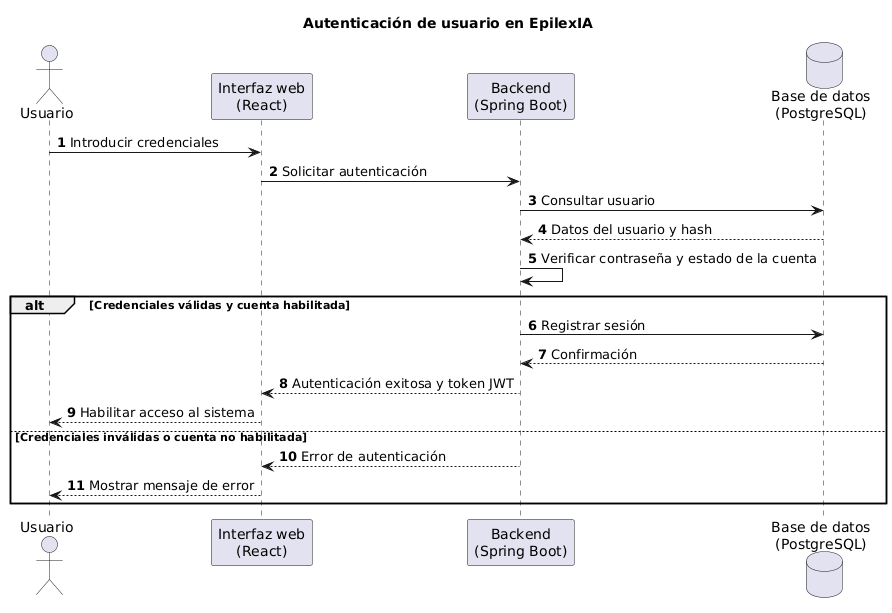
\includegraphics[width=0.95\textwidth]
    {ThesisFigs/secuencia_autenticacion.png}
    \caption{Diagrama de secuencia del proceso de
    autenticación de usuario en EpilexIA.
    Elaboración propia.}
    \label{fig:secuencia-autenticacion}
\end{figure}


\subsection{Registro y preparación de un estudio EEG}
\label{subsec:secuencia-registro-estudio}

El proceso de registro y preparación de un estudio EEG
comprende la identificación del paciente, la creación
del estudio y la incorporación de los archivos asociados.
Estas actividades se desarrollan en etapas diferenciadas,
que permiten gestionar el registro y el procesamiento
de las señales electroencefalográficas.

En la primera etapa, el usuario autorizado selecciona
un paciente existente o incorpora uno nuevo. Posteriormente,
completa la información del estudio, selecciona el archivo
EEG en formato EDF y, cuando corresponde, identifica
al Especialista responsable de su revisión. El \textit{backend}
verifica los datos y registra el estudio con estado inicial
Pendiente.

La Figura~\ref{fig:secuencia-registro-estudio} presenta
las principales interacciones de esta primera etapa.

\begin{figure}[H]
    \centering
    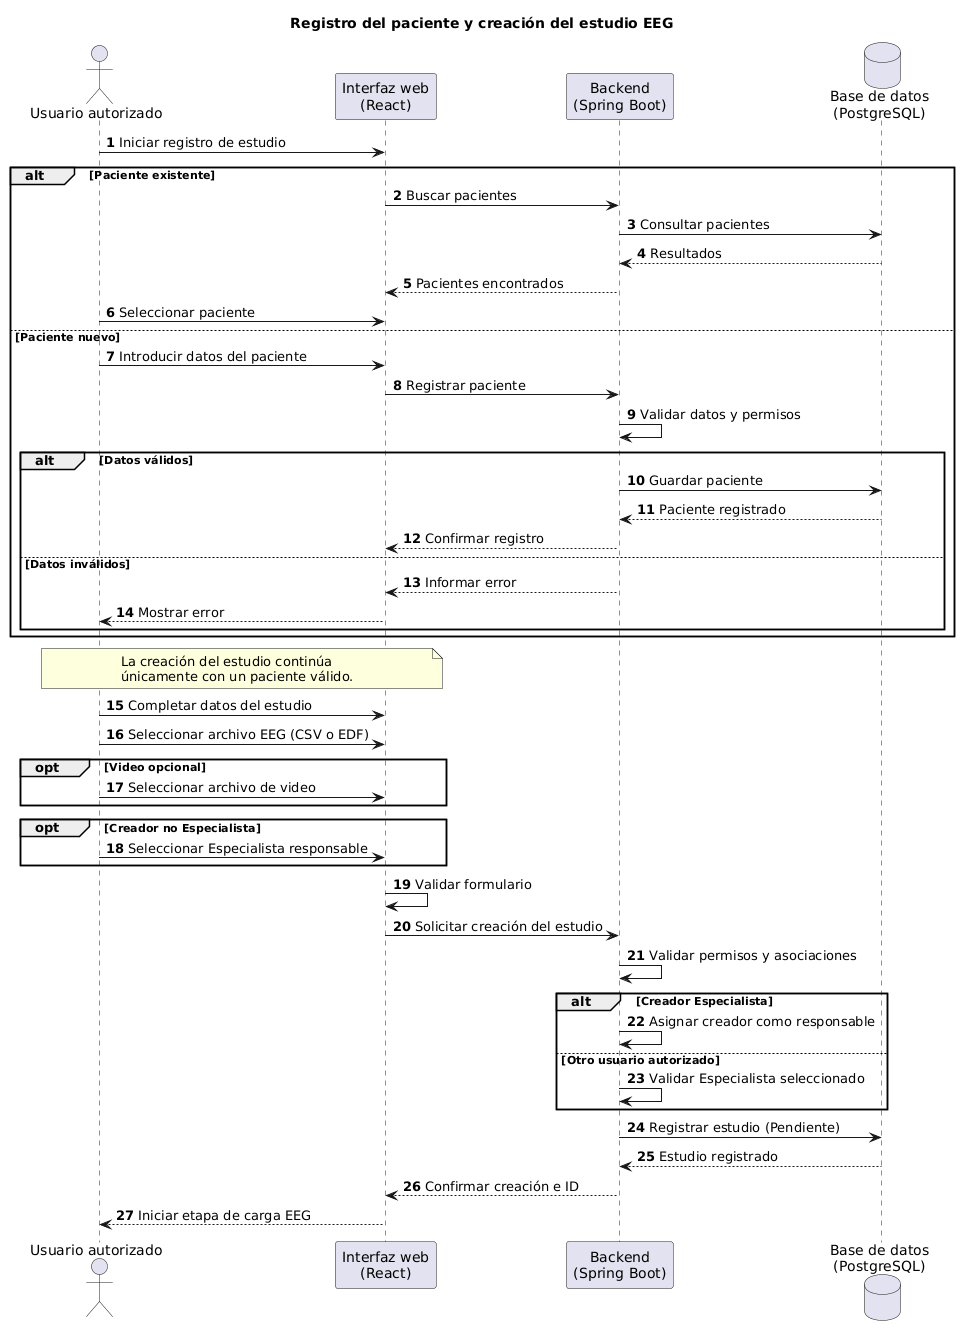
\includegraphics[
        width=\textwidth,
        height=0.82\textheight,
        keepaspectratio
    ]{ThesisFigs/secuencia_registro_estudio.png}
    \caption{Diagrama de secuencia del registro del paciente
    y creación del estudio EEG en EpilexIA.
    Elaboración propia.}
    \label{fig:secuencia-registro-estudio}
\end{figure}

Una vez registrado el estudio, el archivo EEG se transmite
al \textit{backend} mediante fragmentos. Al finalizar la carga,
se inicia el procesamiento correspondiente de manera
asíncrona. Durante esta etapa, la interfaz consulta
periódicamente el estado del estudio hasta obtener
un resultado de procesamiento exitoso o un error.

La Figura~\ref{fig:secuencia-preparacion-eeg} representa
la carga y preparación del archivo EEG, así como
el seguimiento de su estado.

\begin{figure}[H]
    \centering
    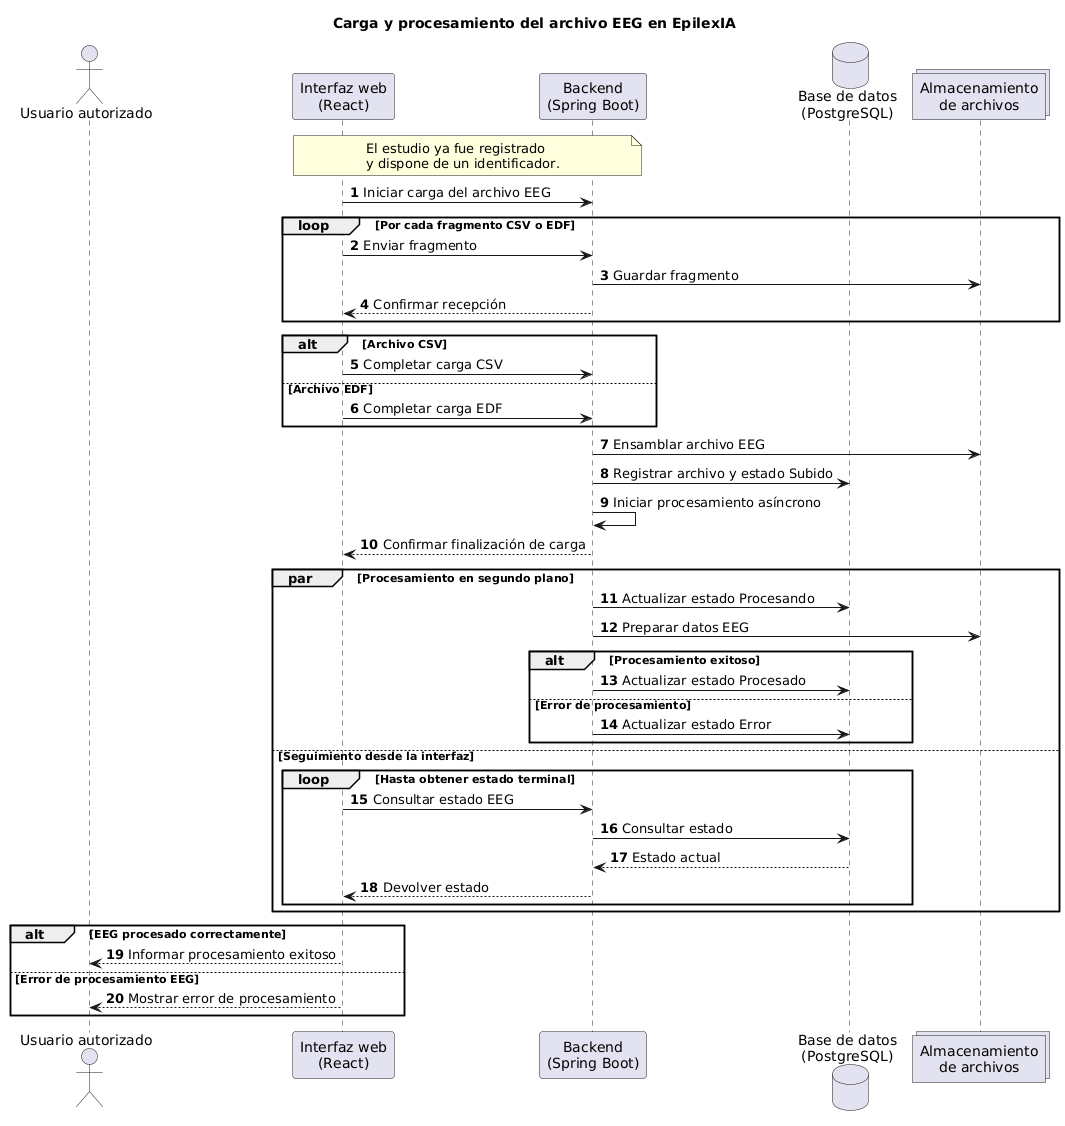
\includegraphics[
        width=\textwidth,
        height=0.82\textheight,
        keepaspectratio
    ]{ThesisFigs/secuencia_carga_procesamiento_eeg.png}
    \caption{Diagrama de secuencia de la carga y
    procesamiento del archivo EEG en EpilexIA.
    Elaboración propia.}
    \label{fig:secuencia-preparacion-eeg}
\end{figure}

Cuando el procesamiento del EEG finaliza correctamente,
el sistema permite continuar con la incorporación
de un video asociado, si corresponde. Los archivos
MP4 se gestionan mediante un procedimiento de carga
y almacenamiento, mientras que los archivos EZVideo
requieren un proceso adicional de conversión a MP4.

La Figura~\ref{fig:secuencia-carga-video} muestra
las interacciones correspondientes a la carga y
preparación del video, incluyendo el seguimiento
de la conversión cuando se utiliza el formato EZVideo.

\begin{figure}[H]
    \centering
    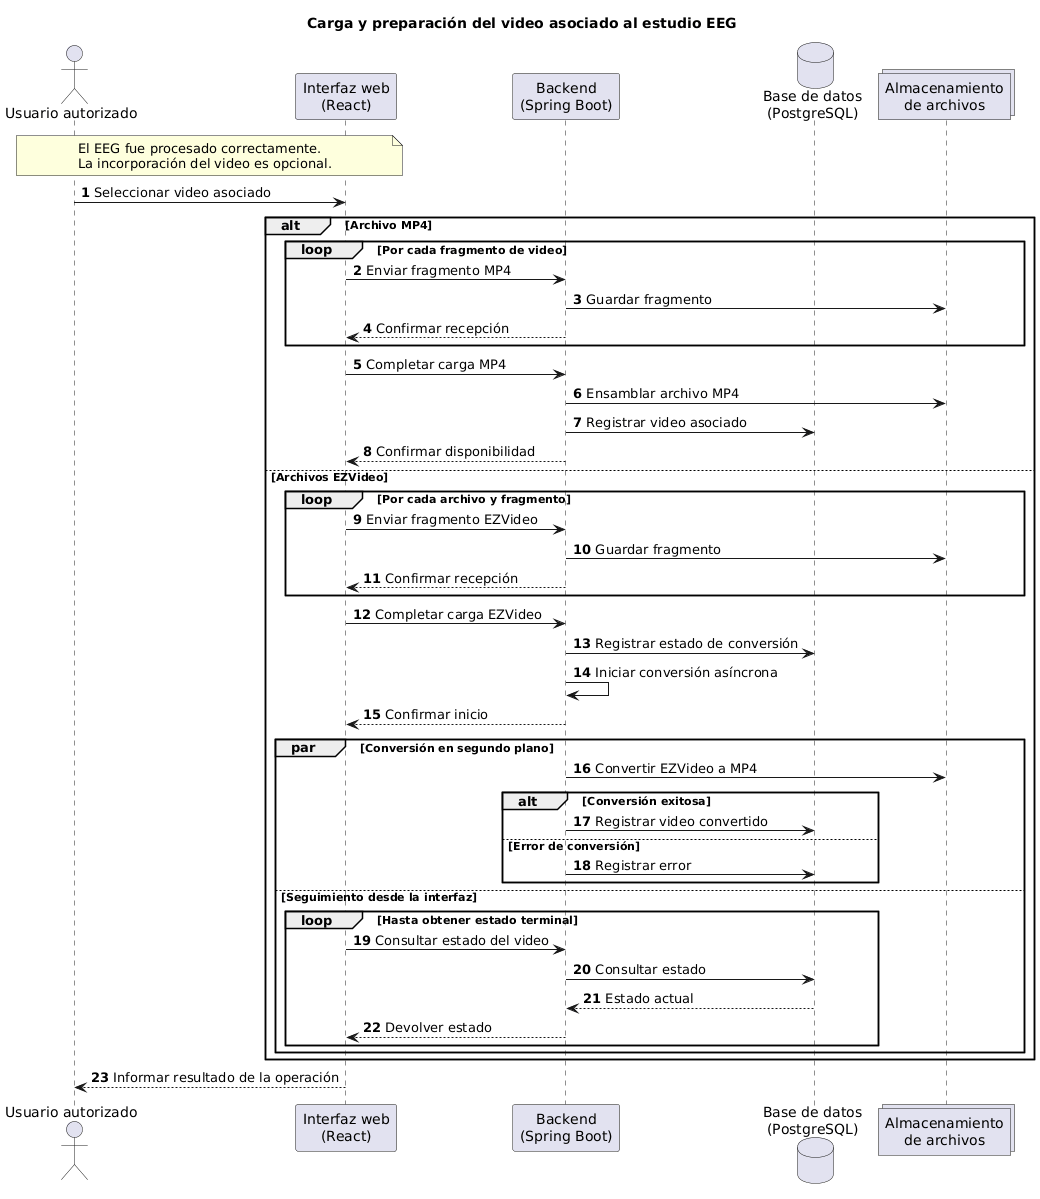
\includegraphics[
        width=\textwidth,
        height=0.82\textheight,
        keepaspectratio
    ]{ThesisFigs/secuencia_carga_video.png}
    \caption{Diagrama de secuencia de la carga y
    preparación del video asociado a un estudio EEG.
    Elaboración propia.}
    \label{fig:secuencia-carga-video}
\end{figure}


\subsection{Visualización de señales EEG}
\label{subsec:secuencia-visualizacion-eeg}

La visualización de señales EEG constituye una de las
funcionalidades principales de EpilexIA, ya que permite
al Especialista examinar los registros
electroencefalográficos asociados a un estudio.

El proceso comienza cuando el usuario autorizado accede
al visualizador. El sistema consulta la información del
estudio, verifica las condiciones de acceso y obtiene
los metadatos necesarios para presentar las señales.
Asimismo, recupera los montajes disponibles y establece
la configuración inicial de visualización.

Las señales EEG se obtienen mediante solicitudes de
segmentos correspondientes a intervalos temporales.
El \textit{backend} recupera los datos almacenados, aplica
los filtros configurados y organiza las derivaciones
según el montaje seleccionado. Posteriormente, la
interfaz web presenta las señales mediante una
representación gráfica multicanal.

La Figura~\ref{fig:secuencia-inicializacion-visualizador-eeg}
representa las principales interacciones correspondientes
al acceso al estudio, la recuperación de información y
la carga inicial de las señales EEG.

\begin{figure}[H]
    \centering
    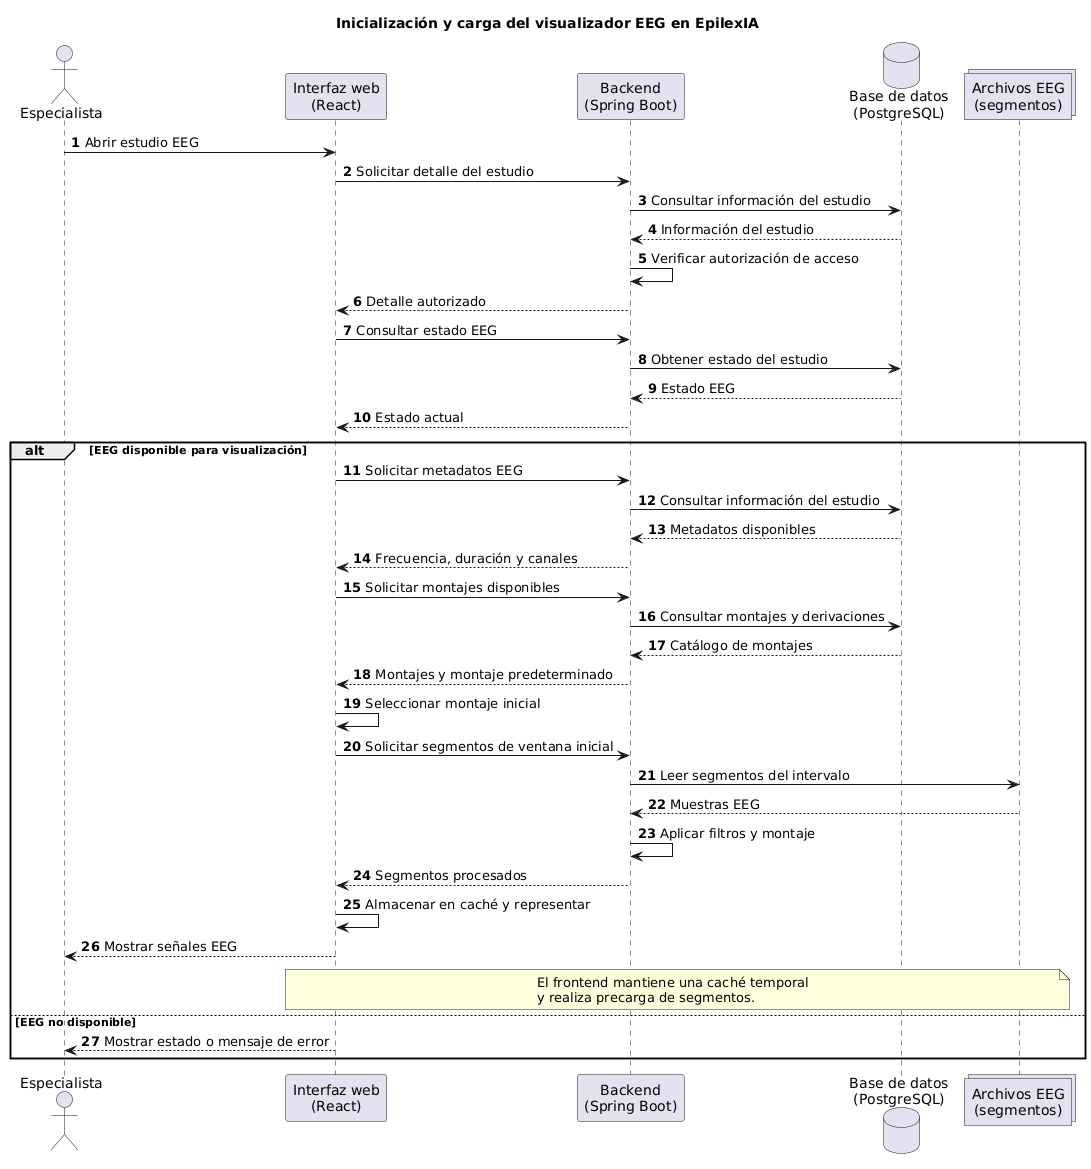
\includegraphics[
        width=\textwidth,
        height=0.82\textheight,
        keepaspectratio
    ]{ThesisFigs/secuencia_inicializacion_visualizador_eeg.png}
    \caption{Diagrama de secuencia de la inicialización
    y carga del visualizador EEG en EpilexIA.
    Elaboración propia.}
    \label{fig:secuencia-inicializacion-visualizador-eeg}
\end{figure}


Durante la revisión del estudio, el Especialista puede
desplazarse entre diferentes intervalos temporales,
seleccionar montajes y ajustar los filtros y la
sensibilidad de las señales. La navegación temporal
contempla dos modalidades complementarias: el
desplazamiento por segundos mediante los controles
de avance y retroceso, y el desplazamiento por ventanas
completas mediante las flechas horizontales del teclado.
La duración de cada ventana puede configurarse entre
5 y 25 segundos.

Asimismo, el Especialista puede modificar la
sensibilidad mediante las flechas verticales del
teclado, lo que permite ajustar la escala de
representación sin interrumpir la revisión del estudio.
Cuando existe un video asociado, la navegación
temporal mantiene la sincronización entre el cursor
EEG y la posición del video.

Para facilitar estas operaciones, el visualizador
mantiene temporalmente en memoria los segmentos
consultados y realiza una precarga de datos. Cuando
la información necesaria se encuentra disponible
en la caché, la representación gráfica puede
actualizarse sin realizar nuevas solicitudes al servidor.

El cambio de montaje o de filtros puede requerir
la recuperación y el procesamiento de nuevos segmentos
por parte del \textit{backend}. En cambio, el ajuste de
sensibilidad modifica la escala vertical de las señales
desde la interfaz web, sin necesidad de recuperar
nuevamente las muestras EEG. La sensibilidad
seleccionada puede conservarse como preferencia
del usuario.

La Figura~\ref{fig:secuencia-interacciones-visualizador-eeg}
presenta las interacciones correspondientes a la
navegación temporal, el cambio de montaje y los
ajustes de filtros y sensibilidad.

\begin{figure}[H]
    \centering
    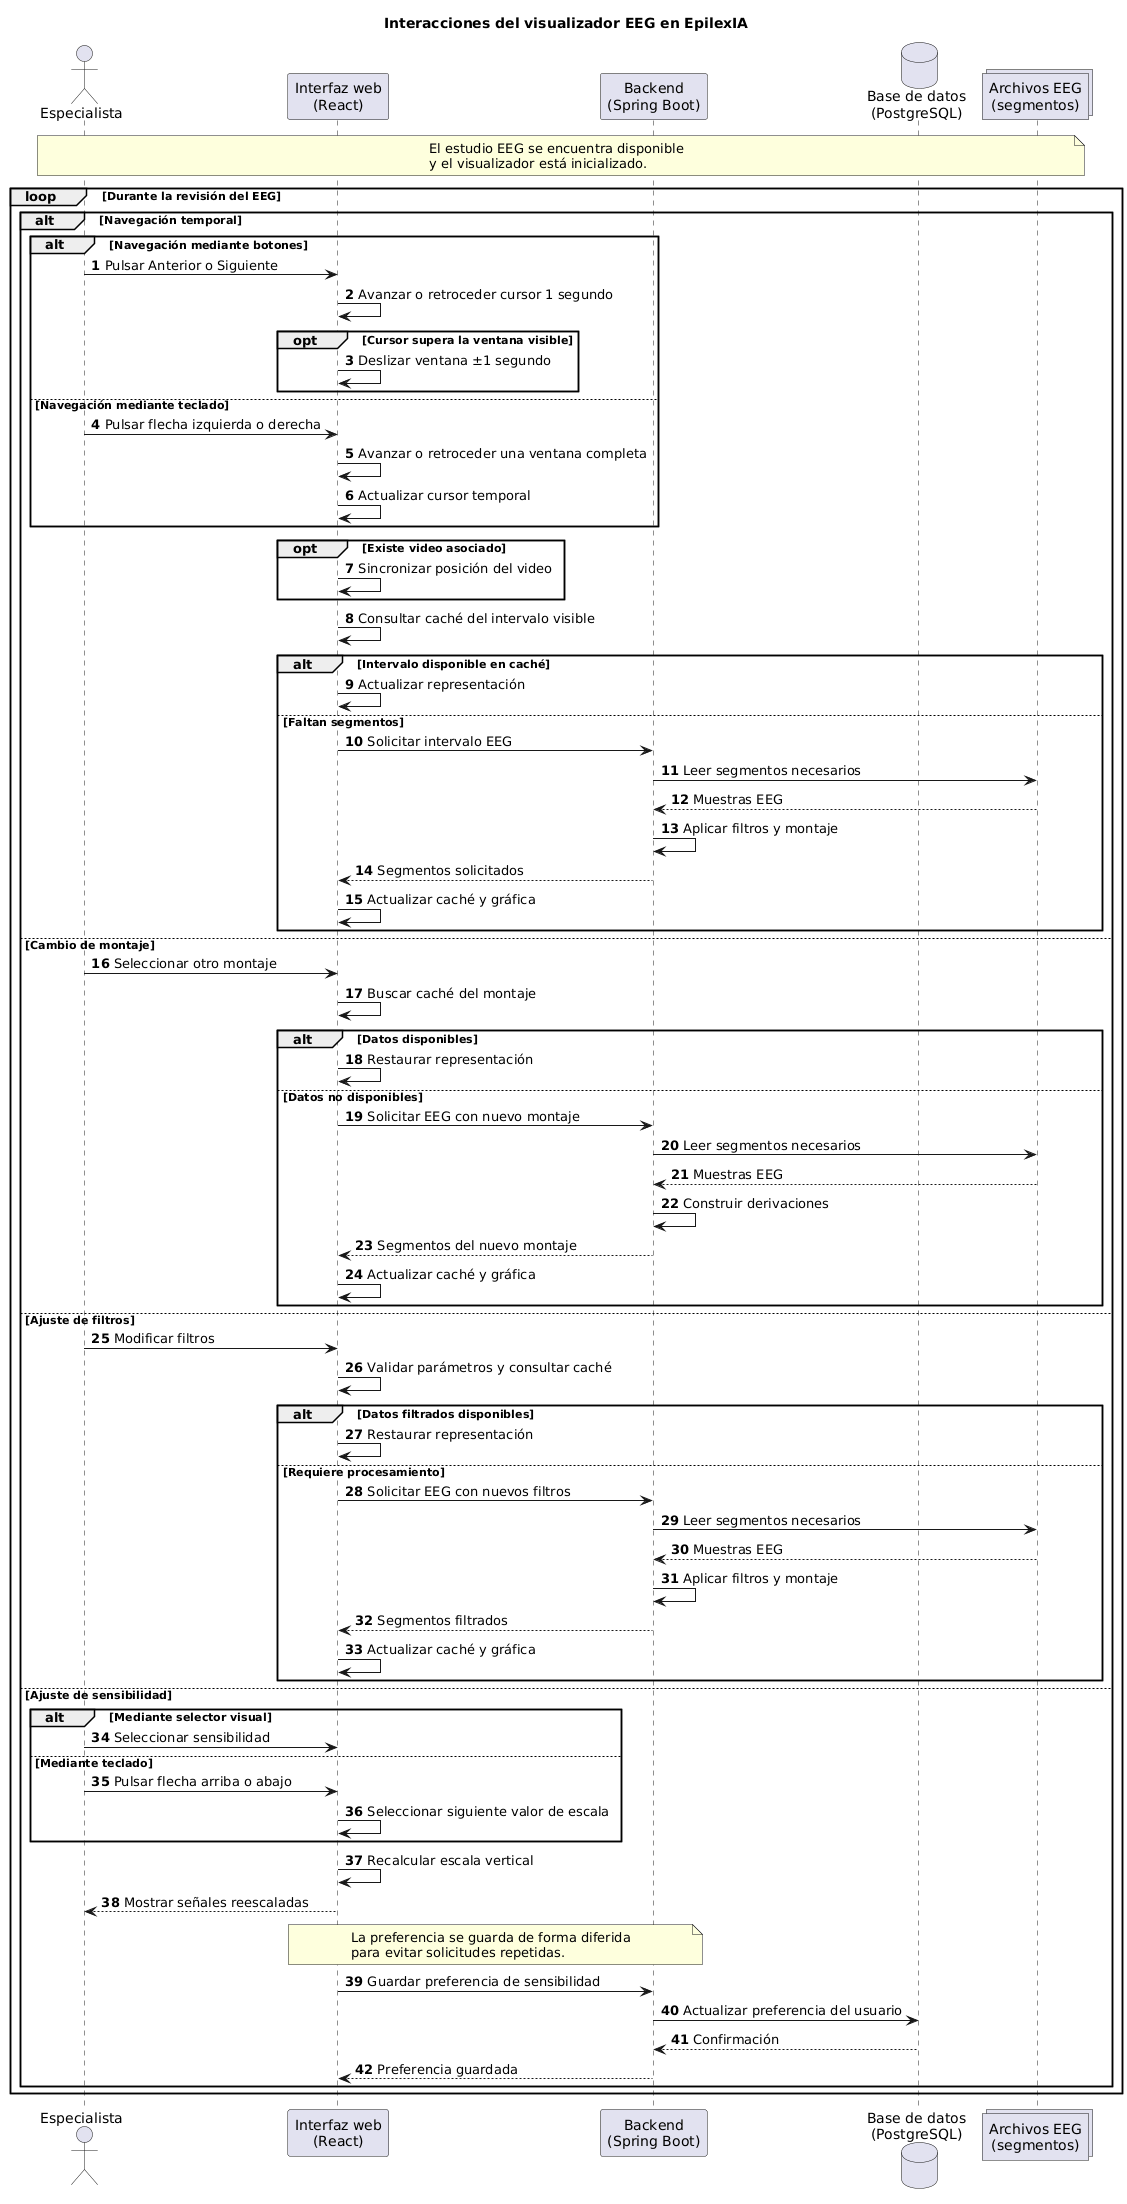
\includegraphics[
        width=\textwidth,
        height=0.82\textheight,
        keepaspectratio
    ]{ThesisFigs/secuencia_interacciones_visualizador_eeg.png}
    \caption{Diagrama de secuencia de las interacciones
    del visualizador EEG en EpilexIA.
    Elaboración propia.}
    \label{fig:secuencia-interacciones-visualizador-eeg}
\end{figure}


\subsection{Procesamiento de estudios mediante inteligencia artificial}
\label{subsec:secuencia-procesamiento-ia}

El procesamiento de estudios EEG mediante inteligencia
artificial constituye una funcionalidad de apoyo al
análisis realizado por el Especialista. Este proceso
permite solicitar el análisis automatizado de un
registro electroencefalográfico y consultar los
resultados obtenidos mediante el servicio de IA
integrado en EpilexIA.

La solicitud se origina en la interfaz web y es
recibida por el \textit{backend} principal, que verifica
los permisos del usuario, las condiciones del
estudio y la disponibilidad del archivo EEG.
Cuando se cumplen las condiciones necesarias,
el \textit{backend} se comunica con la API de IA para
solicitar el procesamiento.

Antes de iniciar una nueva ejecución, el sistema
comprueba si existe una ejecución activa que pueda
ser reutilizada. Cuando corresponde iniciar un
nuevo procesamiento, la API de IA registra la
ejecución y devuelve su identificador y estado
inicial. El \textit{backend} conserva la referencia
correspondiente para permitir su seguimiento.

La Figura~\ref{fig:secuencia-solicitud-ia}
presenta las principales interacciones relacionadas
con la solicitud y el registro de una ejecución
de procesamiento mediante IA.

\begin{figure}[H]
    \centering
    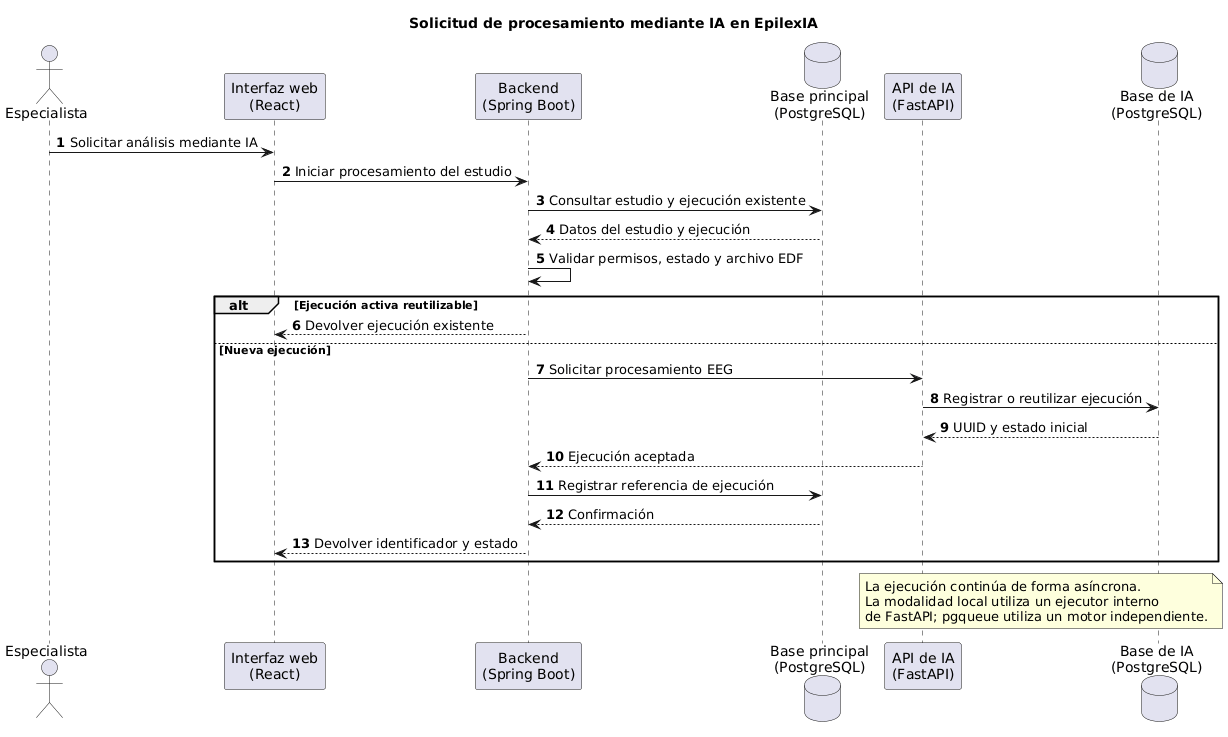
\includegraphics[
        width=\textwidth,
        height=0.82\textheight,
        keepaspectratio
    ]{ThesisFigs/secuencia_solicitud_ia.png}
    \caption{Diagrama de secuencia de la solicitud
    de procesamiento mediante inteligencia artificial
    en EpilexIA. Elaboración propia.}
    \label{fig:secuencia-solicitud-ia}
\end{figure}

El procesamiento se desarrolla de manera asíncrona,
por lo que la aceptación de una solicitud no implica
que el análisis haya finalizado. La ejecución se realiza a través de un motor independiente que obtiene
los trabajos desde una cola persistente.

Durante el procesamiento, la interfaz web consulta
periódicamente el estado de la ejecución. El \textit{backend}
obtiene la información correspondiente y, cuando
resulta necesario, consulta el estado actualizado
mediante la API de IA. Este mecanismo permite
identificar la finalización satisfactoria del
procesamiento o la ocurrencia de errores.

Una vez completada correctamente la ejecución,
el sistema permite recuperar los resultados
almacenados por el servicio de IA y presentarlos
al Especialista. Una ejecución exitosa puede
producir una lista vacía de anomalías, lo que
indica que no se registraron resultados que
cumplieran los criterios de detección establecidos
para dicha ejecución.

La Figura~\ref{fig:secuencia-resultados-ia}
representa el seguimiento del procesamiento
y la posterior consulta de los resultados
obtenidos mediante inteligencia artificial.

\begin{figure}[H]
    \centering
    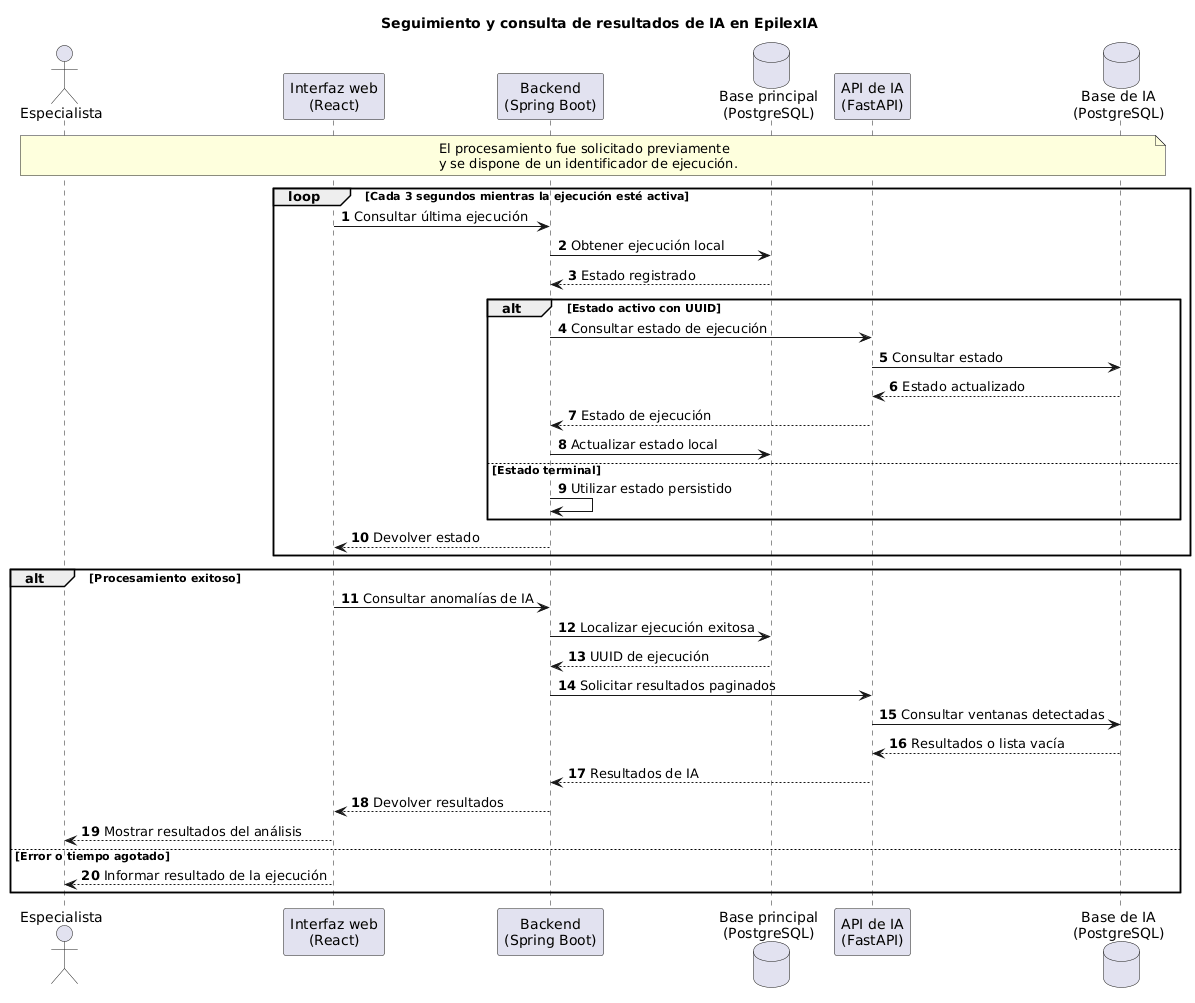
\includegraphics[
        width=\textwidth,
        height=0.82\textheight,
        keepaspectratio
    ]{ThesisFigs/secuencia_resultados_ia.png}
    \caption{Diagrama de secuencia del seguimiento
    y consulta de resultados de inteligencia
    artificial en EpilexIA. Elaboración propia.}
    \label{fig:secuencia-resultados-ia}
\end{figure}

Los resultados obtenidos mediante IA constituyen
información complementaria para la revisión
del estudio y se mantienen diferenciados de
las anotaciones manuales. Su interpretación
clínica corresponde al Especialista, por lo
que el procesamiento automatizado no sustituye
su criterio profesional.


\subsection{Elaboración y cierre de informes clínicos}
\label{subsec:secuencia-informes-clinicos}

La elaboración de informes clínicos constituye una
de las actividades principales realizadas por los
Especialistas durante la revisión de los estudios
electroencefalográficos. EpilexIA permite asociar
informes a un estudio EEG y mantener identificado
al profesional responsable de su elaboración.

El proceso comienza con la consulta de los informes
disponibles para el estudio. Un Especialista autorizado
puede acceder a los informes asociados y, cuando se
cumplen las condiciones correspondientes, crear
su propio informe. La creación genera un documento
en estado Borrador, inicialmente sin contenido clínico,
evitando que se reutilice información perteneciente
a informes elaborados por otros profesionales.

La Figura~\ref{fig:secuencia-creacion-informe}
presenta las interacciones involucradas en la
consulta y creación de informes clínicos.

\begin{figure}[H]
    \centering
    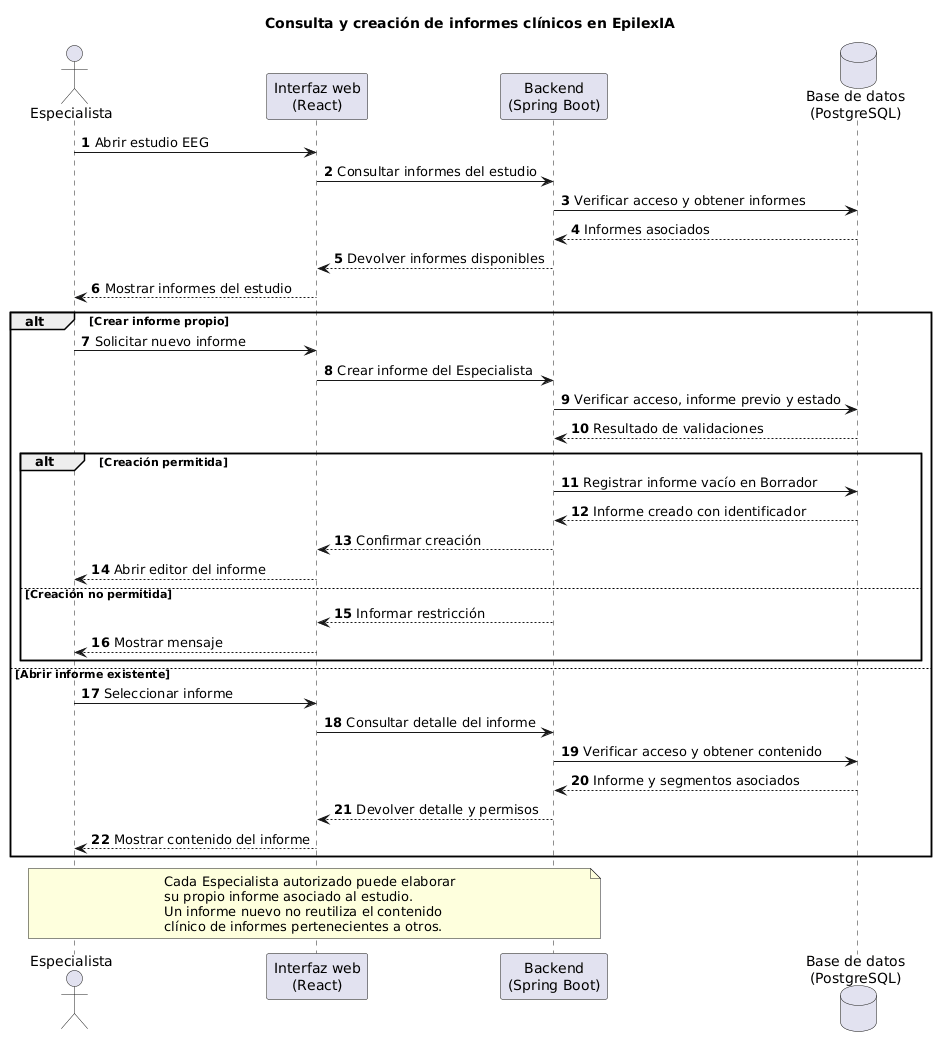
\includegraphics[
        width=\textwidth,
        height=0.82\textheight,
        keepaspectratio
    ]{ThesisFigs/secuencia_creacion_informe.png}
    \caption{Diagrama de secuencia de la consulta
    y creación de informes clínicos en EpilexIA.
    Elaboración propia.}
    \label{fig:secuencia-creacion-informe}
\end{figure}

Durante la elaboración del informe, el Especialista
puede completar la información clínica correspondiente
e incorporar segmentos de interés identificados
durante la revisión del estudio EEG. Estos segmentos
pueden proceder de anotaciones manuales o de
resultados obtenidos mediante el procesamiento
por inteligencia artificial.

Las modificaciones realizadas se envían al \textit{backend},
donde se verifican las condiciones necesarias para
autorizar la actualización. Entre estas condiciones
se encuentran la identificación del propietario
del informe y su estado. De esta manera, el sistema
diferencia la edición del informe propio de la
consulta de documentos pertenecientes a otros
profesionales.

La Figura~\ref{fig:secuencia-edicion-informe}
representa las principales interacciones relacionadas
con la edición y actualización de informes clínicos.

\begin{figure}[H]
    \centering
    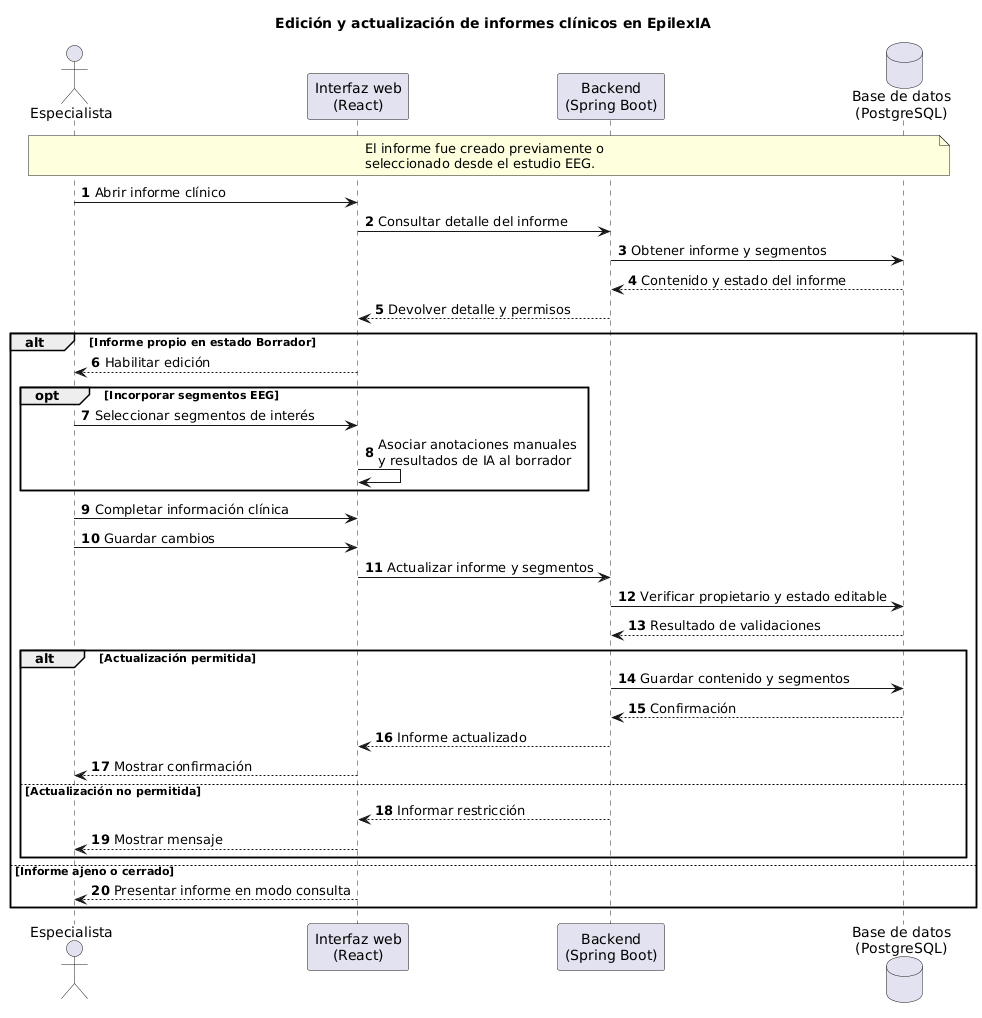
\includegraphics[
        width=\textwidth,
        height=0.82\textheight,
        keepaspectratio
    ]{ThesisFigs/secuencia_edicion_informe.png}
    \caption{Diagrama de secuencia de la edición
    y actualización de informes clínicos en EpilexIA.
    Elaboración propia.}
    \label{fig:secuencia-edicion-informe}
\end{figure}

Una vez finalizada la elaboración del informe,
el Especialista responsable puede solicitar su cierre.
Esta operación requiere una validación específica,
diferente de la utilizada para guardar los cambios
durante la edición. Cuando se cumplen las condiciones establecidas, el sistema actualiza el informe al estado Cerrado y registra la fecha y hora correspondientes al cierre.

El cierre impide que el contenido clínico continúe
modificándose mediante el flujo ordinario de edición.
No obstante, el informe permanece disponible para
su consulta por parte de los usuarios autorizados.

Asimismo, EpilexIA permite generar una representación
del informe en formato PDF. Esta operación recupera
la información clínica y los segmentos asociados,
sin modificar el contenido del documento almacenado.

La Figura~\ref{fig:secuencia-cierre-informe}
presenta las interacciones correspondientes al
cierre y posterior consulta de informes clínicos.

\begin{figure}[H]
    \centering
    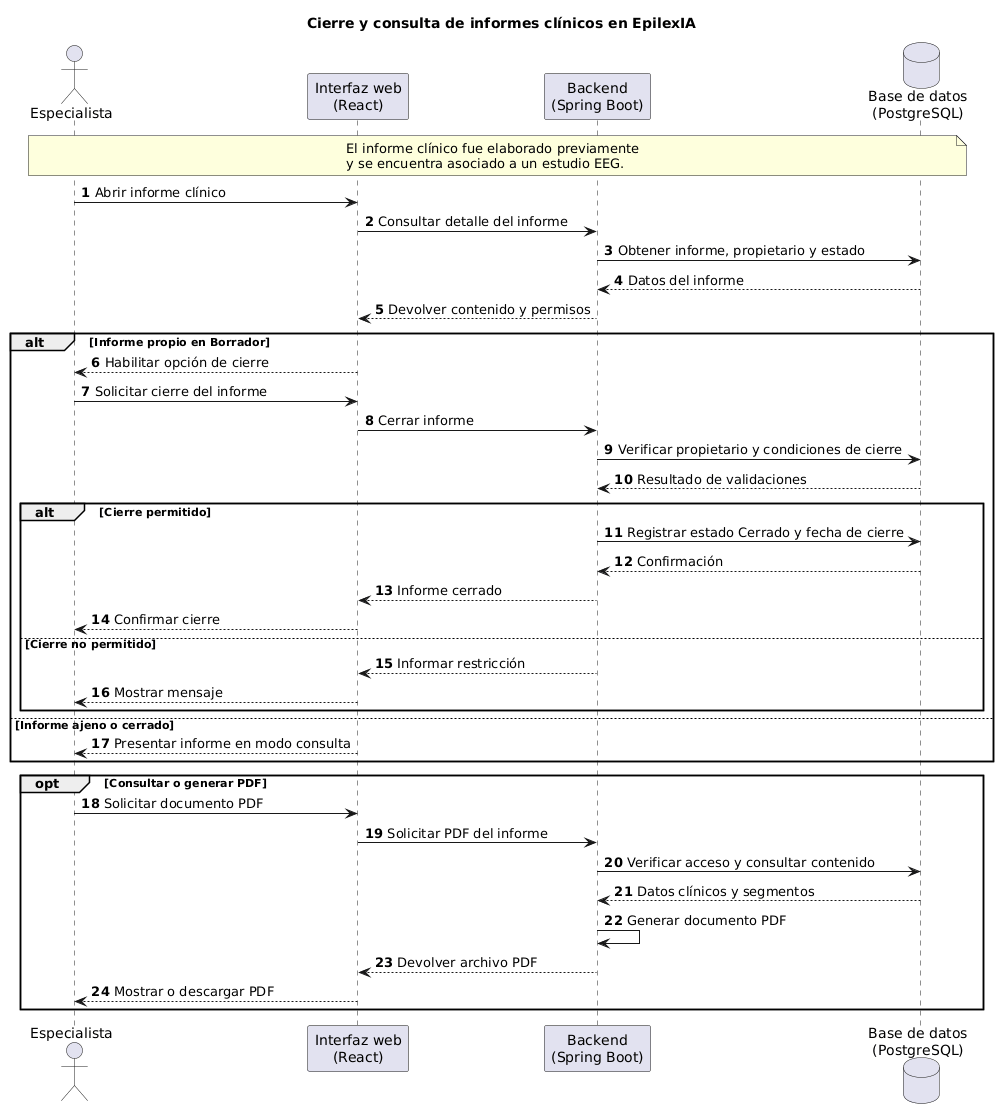
\includegraphics[
        width=\textwidth,
        height=0.82\textheight,
        keepaspectratio
    ]{ThesisFigs/secuencia_cierre_informe.png}
    \caption{Diagrama de secuencia del cierre
    y consulta de informes clínicos en EpilexIA.
    Elaboración propia.}
    \label{fig:secuencia-cierre-informe}
\end{figure}

La separación entre creación, edición y cierre
permite conservar la identificación del profesional
responsable, controlar las modificaciones y mantener
la disponibilidad de los informes asociados a un
mismo estudio. Estas características contribuyen
a la organización del trabajo clínico y a la
trazabilidad de la información registrada.


\section{Arquitectura del sistema}
\label{sec:arquitectura-sistema}

La arquitectura de EpilexIA fue diseñada con el propósito de organizar
las funcionalidades del sistema en componentes diferenciados, de acuerdo
con sus responsabilidades dentro del proceso de gestión y análisis de
estudios electroencefalográficos.

La solución adopta una arquitectura web en la que se separan la
interfaz de usuario, la lógica de negocio, la persistencia de la
información y el procesamiento mediante inteligencia artificial.
Esta organización permite que los componentes se comuniquen mediante
interfaces definidas, manteniendo diferenciadas las operaciones
relacionadas con la gestión clínica y aquellas destinadas al
procesamiento automatizado de las señales EEG.

El diseño contempla la interacción entre los usuarios y la aplicación
web, la administración de la información asociada con pacientes y
estudios, el acceso a los archivos electroencefalográficos y la
integración de los resultados generados mediante inteligencia
artificial.

\subsection{Arquitectura general}
\label{subsec:arquitectura-general}

EpilexIA se organiza mediante una arquitectura cliente-servidor,
complementada con componentes especializados para el procesamiento
de señales EEG.

La interfaz web constituye el punto de acceso de los usuarios
autorizados. Desde ella se realizan las operaciones relacionadas
con la administración del sistema, la gestión de estudios, la
visualización de señales electroencefalográficas y la elaboración
de informes clínicos.

Las solicitudes realizadas desde la interfaz son atendidas por
el \textit{backend} principal, encargado de aplicar las reglas de negocio,
verificar las condiciones de acceso y coordinar las operaciones
necesarias para consultar o modificar la información almacenada.

La persistencia de la información estructurada se organiza mediante dos bases de datos PostgreSQL: una destinada a la gestión clínica y administrativa del sistema, y otra utilizada por el subsistema de inteligencia artificial para almacenar información relacionada con las ejecuciones y sus resultados. Por otra parte, los archivos asociados con los estudios EEG se conservan mediante mecanismos de almacenamiento independientes de las estructuras relacionales.

Para incorporar el análisis automatizado de las señales,
la arquitectura incluye un servicio de inteligencia artificial
integrado mediante una interfaz de programación de aplicaciones.
Este servicio permite gestionar las solicitudes de procesamiento
y consultar los resultados producidos por el componente de análisis.

La arquitectura también contempla la separación entre la
gestión de las ejecuciones de inteligencia artificial y el
procesamiento de las señales. De esta manera, las operaciones
de gestión clínica permanecen diferenciadas de las tareas
computacionales requeridas para el análisis automatizado.

%La Figura~\ref{fig:arquitectura-general} presenta la
%organización general de estos componentes y sus principales
%relaciones.
La Figura~\ref{fig:arquitectura-general} presenta la arquitectura general del sistema EpilexIA, organizada en componentes con responsabilidades diferenciadas. La capa de presentación proporciona la interfaz mediante la cual los usuarios autorizados interactúan con el sistema, mientras que la capa de aplicación concentra las reglas de negocio y coordina las operaciones relacionadas con la gestión de pacientes, estudios electroencefalográficos e informes clínicos.

La persistencia principal comprende los repositorios destinados al almacenamiento de información clínica y administrativa, así como los archivos asociados a los estudios EEG y sus registros de video.

Por su parte, el subsistema de inteligencia artificial dispone de un servicio encargado de recibir y gestionar las solicitudes de análisis, administrar las ejecuciones y proporcionar acceso a los resultados obtenidos. Para la detección automática de crisis epilépticas, las tareas de análisis se registran en una cola persistente y son procesadas por un motor independiente.


En la configuración actualmente utilizada, el procesamiento destinado a la detección automática de crisis epilépticas se encuentra asignado al motor independiente. La coordinación entre este componente y el servicio de IA se establece mediante un repositorio compartido, diseñado para administrar las tareas pendientes, registrar los estados de ejecución y almacenar los resultados del análisis. Por otra parte, la arquitectura contempla la generación de espectrogramas DSA directamente en el servicio de IA, de forma independiente de la detección de crisis.


Esta organización establece una separación de responsabilidades entre los componentes del sistema y permite identificar los mecanismos de integración de la plataforma web con los servicios de inteligencia artificial, sin vincular la representación arquitectónica con tecnologías específicas de implementación. En este contexto, el presente trabajo de tesis se centra en el desarrollo de la plataforma web y en la integración del subsistema de inteligencia artificial, mientras que el desarrollo y el entrenamiento de los modelos de detección, a cargo del equipo de ciencia de datos, y la infraestructura tecnológica forman parte del proyecto integral EpilexIA.


\begin{figure}[H]
    \centering
    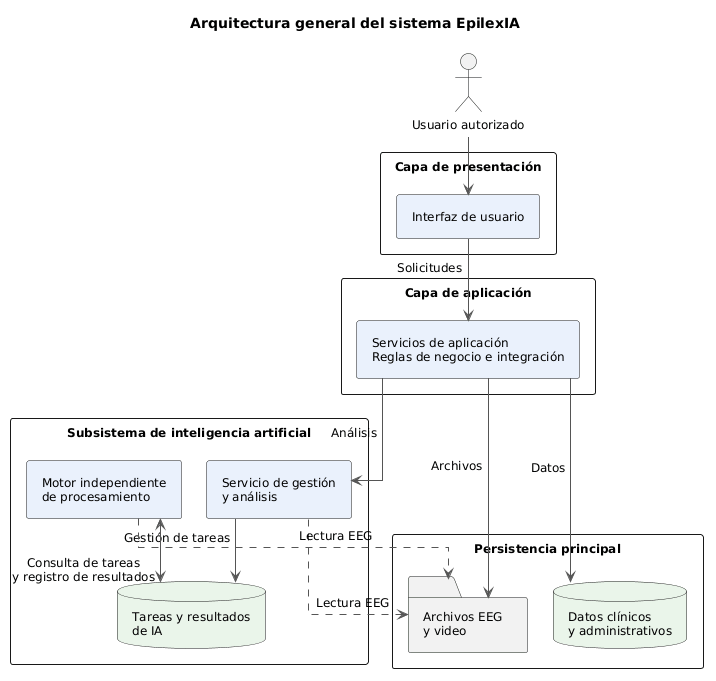
\includegraphics[width=\textwidth]{ThesisFigs/arquitectura_general_epilexia.png}
    \caption{Arquitectura general del sistema EpilexIA.
    Elaboración propia.}
    \label{fig:arquitectura-general}
\end{figure}


\subsection{Componentes de la arquitectura}
\label{subsec:componentes-arquitectura}

La arquitectura de EpilexIA está conformada por componentes
que cumplen responsabilidades específicas dentro del sistema.
Su organización permite separar las operaciones realizadas
por los usuarios, la gestión de la información clínica, el
almacenamiento de archivos y el procesamiento automatizado
de señales EEG.

Como se observa en la Figura~\ref{fig:arquitectura-general},
los componentes principales se distribuyen entre la capa
de presentación, la capa de aplicación, la persistencia
de datos y archivos, y el subsistema de inteligencia
artificial.

\subsubsection{Capa de presentación}

La capa de presentación corresponde a la interfaz web
desarrollada con React y TypeScript. Constituye el punto
de interacción entre los usuarios autorizados y las
funcionalidades disponibles en EpilexIA.

Este componente permite acceder a las operaciones de administración, gestionar la información de pacientes en el contexto de los estudios EEG, visualizar las señales electroencefalográficas, consultar los resultados del procesamiento mediante inteligencia artificial y elaborar informes clínicos.

La interfaz organiza las funcionalidades disponibles de
acuerdo con los permisos del usuario autenticado y
se comunica con el \textit{backend} principal mediante solicitudes
a una API REST.

\subsubsection{Capa de aplicación}

La capa de aplicación está representada por el \textit{backend} principal, desarrollado en Java mediante Spring Boot y preparado para su despliegue como una aplicación WAR sobre el servidor de aplicaciones WildFly.

Este componente concentra las reglas de negocio
relacionadas con la gestión de usuarios, pacientes,
estudios EEG, informes clínicos y eventos de auditoría.
Asimismo, verifica las condiciones de autorización
necesarias para ejecutar las operaciones solicitadas
desde la interfaz web.

El \textit{backend} también coordina el acceso a los datos
persistentes, la gestión de los archivos asociados
con los estudios y la comunicación con el servicio
de inteligencia artificial.

Esta organización permite mantener las validaciones
y las reglas de acceso en el servidor, independientemente
de los controles disponibles en la interfaz de usuario.

\subsubsection{Persistencia de datos y archivos}

La arquitectura contempla mecanismos diferenciados
para almacenar la información estructurada del sistema
y los archivos utilizados durante el análisis de los
estudios EEG.

La base de datos principal, implementada mediante
PostgreSQL, almacena la información correspondiente
a usuarios, pacientes, estudios, informes clínicos,
permisos y registros de auditoría, así como las
relaciones necesarias entre estas entidades.

Por otra parte, los archivos asociados con los
estudios, como los registros electroencefalográficos
y los videos, se conservan mediante mecanismos
de almacenamiento de archivos.

Esta separación permite que la base de datos
mantenga las referencias y los metadatos necesarios
para relacionar los archivos con los estudios,
sin incorporar directamente su contenido completo
a las estructuras relacionales.

\subsubsection{Subsistema de inteligencia artificial}

El subsistema de inteligencia artificial constituye
un conjunto de componentes especializados que
permiten incorporar el procesamiento automatizado
de señales EEG al funcionamiento de EpilexIA.


La comunicación con este subsistema se realiza mediante una API desarrollada con FastAPI, que recibe las solicitudes provenientes del \textit{backend} principal y proporciona los mecanismos necesarios para consultar el estado de las ejecuciones y recuperar los resultados almacenados. La arquitectura contempla, además, la ejecución de nuevas tareas de procesamiento mediante los componentes especializados del subsistema.


El subsistema dispone de una base de datos
PostgreSQL destinada a gestionar la información
relacionada con las ejecuciones de procesamiento
y sus resultados.

Las solicitudes pendientes se gestionan mediante una cola persistente en la base de datos de IA, denominada \texttt{pgqueue}, y son atendidas por un motor de procesamiento independiente.


La arquitectura tiene como propósito facilitar la recuperación y consulta de los resultados obtenidos mediante inteligencia artificial, de manera que puedan utilizarse como información complementaria durante la revisión de los estudios EEG.  La verificación del ciclo completo, desde la solicitud del análisis hasta la presentación de nuevos resultados, se documenta en el Capítulo~\ref{pruebas_evaluacion}.


El desarrollo y entrenamiento del modelo de
inteligencia artificial no forman parte del alcance
de este trabajo, cuya participación
se concentra en su integración con los componentes
del sistema y en la presentación de los resultados
para su revisión por parte del Especialista.


\subsection{Comunicación entre componentes}
\label{subsec:comunicacion-componentes}

La comunicación entre los componentes de EpilexIA se
organiza a partir de las solicitudes realizadas por
los usuarios mediante la interfaz web. Estas solicitudes
son atendidas por el \textit{backend} principal, que coordina
las operaciones necesarias y establece la comunicación
con los mecanismos de persistencia y los servicios
especializados del sistema.

La interacción entre la capa de presentación y la
capa de aplicación se realiza mediante una API REST.
A través de esta interfaz, el \textit{frontend} envía las
solicitudes relacionadas con la autenticación,
la gestión de pacientes y estudios EEG, la consulta
de señales electroencefalográficas y la elaboración
de informes clínicos.

El \textit{backend} recibe estas solicitudes, verifica las
condiciones de acceso correspondientes y ejecuta
las reglas de negocio asociadas con cada operación.
Posteriormente, devuelve las respuestas necesarias
para que la interfaz actualice la información
presentada al usuario.

Para las operaciones que requieren información
persistente, el \textit{backend} interactúa con la base
de datos principal PostgreSQL. Esta comunicación
permite consultar y actualizar los registros
relacionados con usuarios, pacientes, estudios,
informes y eventos de auditoría.

En el caso de los archivos asociados con los
estudios EEG, el \textit{backend} coordina las operaciones
de almacenamiento y recuperación de los datos
necesarios para su posterior procesamiento
y visualización. La información estructurada
que identifica y relaciona estos archivos
con los estudios se conserva en la base de
datos principal.

La comunicación con el subsistema de inteligencia
artificial se establece mediante la API desarrollada
con FastAPI. Cuando se solicita el procesamiento
automatizado de un estudio, el \textit{backend} principal
verifica las condiciones necesarias y transmite
la solicitud al servicio de IA.


La arquitectura contempla el procesamiento asíncrono de las solicitudes de análisis, de manera que la operación inicial no requiera mantener al usuario esperando hasta la finalización del procesamiento. Para ello, se dispone de mecanismos destinados a consultar el estado de las ejecuciones y recuperar los resultados almacenados cuando estén disponibles.


Dentro del subsistema de IA, las ejecuciones pendientes son atendidas por un motor independiente
que utiliza la base de datos de IA para gestionar
los trabajos y registrar sus resultados.


Los resultados de inteligencia artificial almacenados pueden recuperarse mediante la comunicación entre el \textit{backend} principal y la API de IA. Posteriormente, la interfaz web permite presentarlos en el contexto del estudio correspondiente, de manera que el Especialista pueda examinarlos junto con las señales EEG. Este mecanismo contempla tanto la consulta de resultados existentes como la recuperación de nuevos resultados cuando finalicen las ejecuciones de procesamiento.


Esta organización permite mantener una
comunicación diferenciada entre los componentes
encargados de la gestión del sistema y aquellos
destinados al procesamiento automatizado,
conservando al \textit{backend} principal como punto
de coordinación de las operaciones solicitadas
desde la interfaz web.


\section{Diseño de la base de datos}
\label{sec:diseno-base-datos}

El diseño de persistencia de EpilexIA contempla
la separación de la información clínica y operativa
del sistema respecto de los datos utilizados para
coordinar el procesamiento mediante inteligencia
artificial. Para ello, se emplean dos bases de datos
relacionales PostgreSQL, con responsabilidades
diferenciadas.

\subsection{Organización general de los datos}
\label{subsec:organizacion-datos}

La base de datos principal almacena la información
estructurada necesaria para la gestión de usuarios,
pacientes, estudios EEG, informes médicos, anomalías
registradas y demás operaciones de la plataforma.
Esta información permite establecer las relaciones
entre los estudios y los profesionales que intervienen
en su registro, revisión e interpretación.

Por otra parte, el subsistema de inteligencia artificial
dispone de una base de datos independiente, destinada
a gestionar las solicitudes de procesamiento, sus
estados de ejecución y los resultados obtenidos.
Esta base de datos permite coordinar las actividades
entre la API de inteligencia artificial y el motor
de procesamiento.

Los archivos que contienen las señales EEG y los
videos asociados se conservan en un almacenamiento
de archivos independiente de las tablas relacionales.
De esta manera, la información estructurada del
sistema puede relacionarse con los registros
electroencefalográficos sin requerir que el contenido
completo de dichos archivos se almacene directamente
en la base de datos clínica.


\subsection{Modelo de datos clínicos}
\label{subsec:modelo-datos-clinicos}

El modelo de datos clínicos de EpilexIA se estructura
principalmente alrededor de las entidades
\texttt{patient} y \texttt{study}, que representan,
respectivamente, a los pacientes registrados y sus
estudios electroencefalográficos. La relación entre
ambas entidades es de uno a muchos, dado que un
paciente puede tener varios estudios EEG, mientras
que cada estudio corresponde a un único paciente.

La entidad \texttt{study} constituye el núcleo del modelo y mantiene referencias a los usuarios que intervienen en la gestión del estudio. Cada estudio debe estar asociado obligatoriamente a un usuario responsable, cuya pertenencia al rol Especialista se verifica mediante las reglas de negocio del \textit{backend} durante su creación. Asimismo, puede incluir de manera opcional un técnico encargado de su registro. La entidad también conserva información sobre el estado del estudio, su anulación, reactivación y disponibilidad de video.

Los archivos asociados a cada estudio se representan mediante la entidad
\texttt{study\_file}, relacionada con el catálogo
\texttt{study\_file\_type}, que permite identificar el formato
correspondiente. Esta estructura admite múltiples archivos por estudio,
incluyendo señales EEG y videos, y conserva metadatos técnicos como la
duración, la frecuencia de muestreo y los canales disponibles.
Estos metadatos se registran o completan durante las operaciones de carga
y procesamiento de los archivos, de acuerdo con las características y
los mecanismos de lectura de cada formato.

Para representar las configuraciones de visualización,
el modelo incorpora las entidades \texttt{eeg\_montage}
y \texttt{eeg\_montage\_channel}. La primera define los
montajes electroencefalográficos disponibles, mientras
que la segunda establece los canales o derivaciones
que componen cada montaje y su orden de presentación.

Los hallazgos registrados durante la revisión de un
estudio se organizan en dos estructuras diferenciadas.
La entidad \texttt{anomaly} representa intervalos de
señal identificados manualmente o mediante inteligencia
artificial, con referencias opcionales a su clasificación
y montaje. Por otra parte, \texttt{study\_eeg\_event}
almacena eventos temporales asociados al estudio,
utilizando tipos predefinidos o personalizados.


La elaboración de informes médicos se modela mediante las entidades \texttt{report}, \texttt{study\_report} y \texttt{report\_segment}. La entidad \texttt{report} almacena el contenido clínico del informe, mientras que \texttt{study\_report} establece la asociación entre el estudio, el Especialista y el informe correspondiente. Esta relación permite la existencia de informes elaborados por diferentes Especialistas para un mismo estudio, con la restricción de un único informe por Especialista dentro de dicho estudio.


Finalmente, \texttt{report\_segment} permite asociar
a cada informe los intervalos de señal considerados
relevantes, conservando información sobre su ubicación
temporal y, cuando corresponde, sus referencias a
anomalías, montajes o ejecuciones de inteligencia
artificial.

El modelo se complementa con estructuras de control
de acceso, compartición de estudios y auditoría,
que permiten relacionar las operaciones clínicas con
los usuarios participantes y conservar información
para su trazabilidad.


La Figura~\ref{fig:er-pacientes-estudios}
presenta las principales entidades relacionadas
con el registro de pacientes, la gestión de estudios
electroencefalográficos, sus archivos asociados
y las configuraciones de montaje EEG.

Por su parte, la Figura~\ref{fig:er-informes-anomalias}
representa las relaciones entre los estudios,
las anomalías, los eventos EEG y los informes
clínicos elaborados por los especialistas.
Ambas figuras constituyen vistas simplificadas
del modelo relacional, en las que se priorizan
las entidades y asociaciones más relevantes
para comprender el diseño del sistema.


\begin{figure}[H]
    \centering
    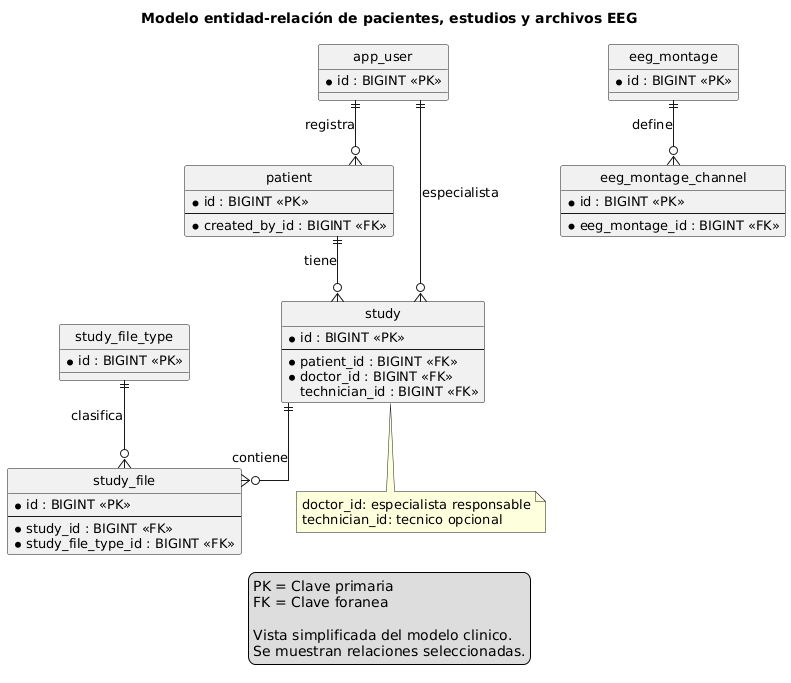
\includegraphics[width=\textwidth]{ThesisFigs/er_pacientes_estudios.png}
    \caption{Modelo entidad-relación de pacientes,
    estudios y archivos EEG de EpilexIA.}
    \label{fig:er-pacientes-estudios}
\end{figure}

\begin{figure}[H]
    \centering
    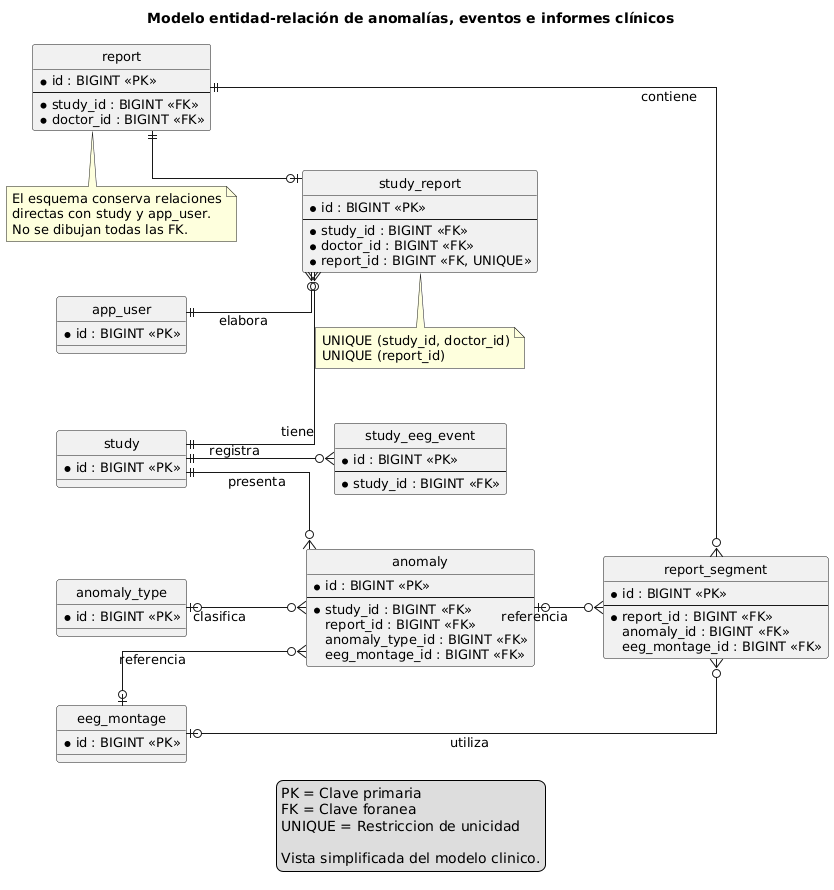
\includegraphics[width=\textwidth]{ThesisFigs/er_informes_anomalias.png}
    \caption{Modelo entidad-relación de anomalías,
    eventos e informes clínicos de EpilexIA.}
    \label{fig:er-informes-anomalias}
\end{figure}


\subsection{Modelo de datos del procesamiento de inteligencia artificial}
\label{subsec:modelo-datos-ia}

El subsistema de inteligencia artificial de EpilexIA utiliza una base de datos PostgreSQL independiente de la base de datos clínica principal. Su diseño permite registrar las solicitudes de procesamiento de señales EEG, controlar los estados de ejecución, almacenar los resultados obtenidos y conservar información de retroalimentación proporcionada por los especialistas. El esquema comprende seis tablas principales, cuya estructura es administrada mediante migraciones de la API de inteligencia artificial desarrollada con FastAPI.

La entidad central del modelo es \texttt{ai\_executions}, que representa cada solicitud de análisis electroencefalográfico. Cada ejecución se identifica mediante un UUID y conserva información sobre el estudio asociado, el modelo utilizado, su versión, el umbral mínimo de probabilidad y la ubicación del archivo EEG que debe procesarse. Asimismo, registra el estado de ejecución, las fechas de inicio y finalización y los datos operativos necesarios para identificar posibles errores.

El ciclo de vida de una ejecución se representa mediante estados como \texttt{QUEUED}, \texttt{RUNNING}, \texttt{SUCCESS}, \texttt{FAILED}, \texttt{TIMEOUT} y \texttt{CANCELLED}. Adicionalmente, el subsistema contempla el estado interno \texttt{CANCEL\_REQUESTED}, utilizado para coordinar las solicitudes de cancelación durante el procesamiento mediante cola.

La configuración del modelo activo se administra mediante la entidad \texttt{ai\_model\_params}, que almacena parámetros como el nombre, la versión y el umbral mínimo de probabilidad de crisis. Al registrar una ejecución, estos valores se incorporan a \texttt{ai\_executions}, permitiendo conservar la configuración utilizada en cada procesamiento. Los archivos que contienen los modelos entrenados se mantienen fuera de la base de datos, en un almacenamiento independiente.

Los resultados del análisis se representan mediante la entidad \texttt{ai\_results}, relacionada con \texttt{ai\_executions} mediante una clave foránea. Cada registro corresponde a un intervalo temporal identificado por el procesamiento de inteligencia artificial y conserva su instante inicial, instante final y probabilidad estimada de crisis. El sistema almacena únicamente las ventanas clasificadas positivamente que cumplen el umbral mínimo configurado. Por consiguiente, una ejecución finalizada correctamente puede no generar registros de resultados cuando no se identifican intervalos que satisfagan dicho criterio.

El modelo incorpora mecanismos para conservar la revisión realizada por los especialistas. La entidad \texttt{ai\_results} dispone de atributos destinados a registrar la validación médica de los intervalos detectados. Por su parte, \texttt{ai\_report\_window\_inclusions} permite asociar los resultados de inteligencia artificial con los informes clínicos en los que fueron incluidos, conservando información descriptiva y de clasificación aportada por el profesional.

Complementariamente, la entidad \texttt{ai\_manual\_annotations} almacena anotaciones realizadas manualmente por los especialistas, incluso cuando no corresponden a intervalos detectados previamente por el modelo. Estas estructuras permiten conservar información de retroalimentación clínica que podría utilizarse en futuros procesos de mejora de los modelos de inteligencia artificial, sin que ello implique la existencia de un mecanismo automático de reentrenamiento en la implementación actual.

La base de datos también contempla la entidad \texttt{ai\_results\_historial}, destinada al almacenamiento histórico de resultados. Esta estructura se encuentra definida en el esquema; el traslado automático de registros hacia ella desde la tabla de resultados activos no está implementado en la versión actual.

La tabla \texttt{ai\_executions} cumple además una función de coordinación entre la API de inteligencia artificial y el motor de procesamiento independiente. La API registra las solicitudes pendientes y el motor adquiere los trabajos mediante operaciones transaccionales sobre PostgreSQL. Durante la ejecución se actualizan los estados y las señales de actividad del procesamiento, mientras que al finalizar se registran los resultados y el estado correspondiente.

La vinculación con la base de datos clínica se establece mediante identificadores compartidos a nivel de aplicación. En particular, \texttt{id\_study\_epilex} permite identificar el estudio clínico asociado, mientras que el UUID de la ejecución puede relacionarse con los registros de seguimiento mantenidos por el \textit{backend} principal. Debido a que ambas bases de datos funcionan de manera independiente, estas correspondencias no se implementan mediante claves foráneas entre ellas.

Finalmente, los archivos EEG, los modelos entrenados y los archivos temporales generados durante el procesamiento se conservan en almacenamiento de archivos. Esta separación permite mantener en PostgreSQL los datos estructurados necesarios para la gestión, consulta y trazabilidad de las ejecuciones, sin incorporar directamente los archivos de señales ni los artefactos del modelo.


La Figura~\ref{fig:er-subsistema-ia} presenta
una vista simplificada del modelo entidad-relación
del subsistema de inteligencia artificial de EpilexIA.
Se destacan las relaciones entre las ejecuciones
de procesamiento, los resultados generados y las
ventanas incorporadas a informes clínicos.
Asimismo, se representan las estructuras destinadas
a la configuración del modelo, las anotaciones
manuales y el almacenamiento histórico, diferenciando
las relaciones definidas mediante claves foráneas
de las referencias lógicas gestionadas por la aplicación.


\begin{figure}[H]
    \centering
    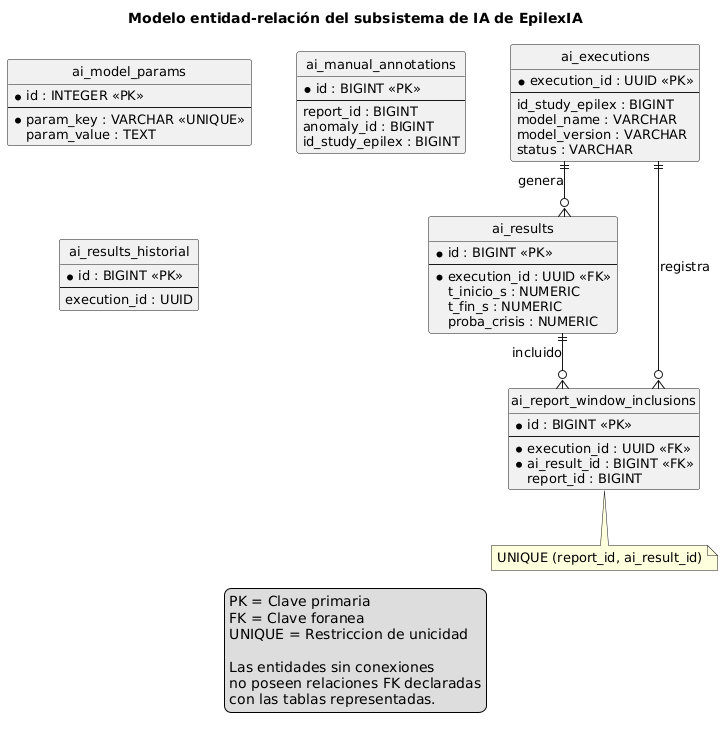
\includegraphics[width=\textwidth]{ThesisFigs/er_subsistema_ia.png}
    \caption{Modelo entidad-relación del subsistema
    de inteligencia artificial de EpilexIA.}
    \label{fig:er-subsistema-ia}
\end{figure}


\subsection{Integridad y persistencia de los datos}
\label{subsec:integridad-persistencia-datos}

El diseño de persistencia de EpilexIA contempla mecanismos
de integridad orientados a mantener la consistencia de
la información clínica y de los registros asociados al
procesamiento mediante inteligencia artificial. Para ello,
las bases de datos PostgreSQL emplean claves primarias,
claves foráneas y restricciones de unicidad que permiten
identificar los registros y controlar sus relaciones.

En la base de datos clínica, las restricciones de integridad
referencial permiten establecer asociaciones entre pacientes,
estudios electroencefalográficos, archivos, anomalías e
informes médicos. Estas relaciones contribuyen a evitar
referencias a registros inexistentes y a mantener la
correspondencia entre los estudios y la información generada
durante su revisión. Asimismo, determinadas restricciones
de unicidad permiten aplicar reglas del modelo, como la
existencia de un único informe por Especialista dentro
de un mismo estudio.

En la base de datos del subsistema de inteligencia artificial,
la integridad referencial se aplica principalmente a las
relaciones entre las ejecuciones de procesamiento, los
resultados obtenidos y los registros de inclusión de ventanas
en informes clínicos. Cada resultado se vincula con la
ejecución que lo generó, permitiendo identificar su origen
y conservar la trazabilidad de los intervalos detectados
por el modelo.

La separación entre la base de datos clínica y la base
de datos de inteligencia artificial implica que sus
correspondencias se gestionan mediante identificadores
compartidos a nivel de aplicación, sin establecer claves
foráneas entre ambas bases. De esta manera, cada subsistema
mantiene sus propias restricciones de integridad y
responsabilidades de persistencia.

Por otra parte, los archivos de señales EEG, los videos
asociados y los modelos entrenados se conservan en
almacenamiento de archivos, mientras que las bases de datos
mantienen los registros estructurados y las referencias
necesarias para su identificación y utilización. Esta
organización evita almacenar directamente archivos de gran
tamaño dentro de las tablas relacionales y permite separar
la gestión de metadatos del almacenamiento de los recursos
utilizados por el sistema.

Finalmente, el diseño incorpora registros de auditoría
y seguimiento de ejecuciones que contribuyen a la
trazabilidad de las operaciones realizadas. Estas
estructuras permiten relacionar las actividades registradas
con sus respectivos usuarios, estudios o procesos, según
corresponda, y proporcionan información para el análisis
de las operaciones del sistema.


\section{Diseño de los servicios e interfaces de integración}
\label{sec:diseno-servicios-integracion}

La integración de los componentes de EpilexIA se organiza
mediante interfaces de comunicación que permiten intercambiar
información entre la aplicación web, el \textit{backend} principal y
el subsistema de inteligencia artificial. Esta organización
establece responsabilidades diferenciadas para la gestión
clínica, el acceso a los estudios electroencefalográficos
y la ejecución de los procesos de análisis automatizado.

La interfaz web, desarrollada con React, consume los servicios
REST expuestos por el \textit{backend} principal, implementado con
Spring Boot y ejecutado sobre WildFly. Este componente
centraliza las operaciones relacionadas con usuarios,
pacientes, estudios EEG, informes médicos y auditoría,
además de gestionar la comunicación con los servicios
de inteligencia artificial.

La integración con el subsistema de inteligencia artificial
se realiza mediante una API independiente desarrollada
con FastAPI. El \textit{backend} principal utiliza esta interfaz
para solicitar análisis, consultar su estado, recuperar
resultados y obtener representaciones complementarias
de las señales EEG, como los espectrogramas.

La API de inteligencia artificial y el motor de procesamiento
se coordinan a través de una base de datos PostgreSQL
compartida por ambos componentes. Esta comunicación permite
gestionar las solicitudes de análisis sin requerir una
conexión HTTP directa entre la API y el motor.

El diseño de las interfaces también contempla mecanismos
de autenticación, validación de solicitudes y tratamiento
de errores, con el propósito de controlar el acceso a
las operaciones y proporcionar respuestas adecuadas
a los componentes consumidores.


\subsection{Servicios del \textit{backend} principal}
\label{subsec:servicios-backend-principal}

El \textit{backend} principal de EpilexIA constituye la capa
encargada de gestionar las operaciones del sistema y
coordinar el intercambio de información entre la interfaz
web, la base de datos clínica, el almacenamiento de
archivos y los servicios de inteligencia artificial.

Este componente fue desarrollado en Java, utilizando
Spring Boot y una arquitectura organizada en controladores
REST, servicios de aplicación y repositorios de
persistencia. Su despliegue se realiza mediante un
artefacto WAR preparado para ejecutarse sobre el
servidor de aplicaciones WildFly.

Los controladores exponen interfaces HTTP orientadas
a recursos, mediante las cuales el \textit{frontend} realiza
operaciones de consulta, registro, actualización y
gestión de información. Estas interfaces utilizan
principalmente mensajes en formato JSON y objetos
de transferencia de datos (DTO), que permiten
separar los contratos de comunicación de las
entidades utilizadas internamente por el sistema.

Los servicios REST se agrupan según sus
responsabilidades funcionales. Entre ellos se
encuentran la autenticación y administración de
usuarios, la gestión de pacientes y estudios EEG,
la recepción de archivos, la recuperación de señales
para su visualización, el registro de anomalías y
eventos, la elaboración de informes médicos y
la consulta de actividades de auditoría.

Para facilitar el intercambio de información,
la mayoría de las respuestas JSON emplea una
estructura común que identifica el resultado de
la operación, un mensaje opcional y los datos
solicitados. Asimismo, las consultas de listados
extensos incorporan mecanismos de paginación,
mientras que la transferencia de archivos utiliza
formatos adecuados a su naturaleza, como
\texttt{multipart/form-data} para las cargas
y respuestas binarias para los documentos generados.

La gestión de los estudios EEG contempla interfaces
para recibir archivos EDF mediante carga
fragmentada. Una vez completada la transferencia,
el \textit{backend} ensambla el archivo y ejecuta su
procesamiento de manera asíncrona. Como resultado,
se generan segmentos comprimidos que posteriormente
pueden recuperarse por índice o intervalo temporal.

Para la visualización de las señales, el \textit{backend}
proporciona servicios de consulta de metadatos,
segmentos, montajes y derivaciones. La resolución
de montajes y la aplicación de filtros digitales
se realizan en el servidor, mientras que la
sensibilidad seleccionada por el usuario interviene
en la representación gráfica efectuada por
la interfaz web.

La seguridad de estas interfaces combina
autenticación mediante \textit{tokens} JWT y autorización
basada en permisos. Adicionalmente, las operaciones
sobre estudios e informes incorporan verificaciones
contextuales que consideran la relación del usuario
con el recurso solicitado. De esta manera, el
acceso no depende únicamente del permiso funcional,
sino también de las condiciones particulares de
cada estudio o informe médico.

Finalmente, el \textit{backend} principal actúa como
intermediario entre la aplicación web y el
subsistema de inteligencia artificial. Para ello,
dispone de servicios que permiten solicitar
ejecuciones, consultar sus estados, recuperar
resultados y obtener espectrogramas, sin exponer
directamente al \textit{frontend} las interfaces internas
de procesamiento.


\begin{table}[H]
\centering
\caption{Interfaces REST representativas del \textit{backend} principal}
\label{tab:interfaces-rest-backend}

\small
\setlength{\tabcolsep}{4pt}
\renewcommand{\arraystretch}{1.3}

\begin{tabular}{|p{2.4cm}|p{6.2cm}|p{4.4cm}|}
\hline
\textbf{Servicio} &
\textbf{Interfaz REST} &
\textbf{Finalidad} \\ \hline

Autenticación &
\texttt{POST /api/auth/login} &
Autenticar al usuario y emitir el \textit{token} de acceso. \\ \hline

Pacientes &
\texttt{POST /api/patients} &
Registrar los datos de un paciente. \\ \hline

Estudios EEG &
\texttt{POST /api/studies} &
Registrar un nuevo estudio electroencefalográfico. \\ \hline

Carga EEG &
\texttt{POST /api/studies/\{id\}/eeg/}
\newline
\texttt{upload-chunk-edf} &
Recibir fragmentos de un archivo EEG en formato EDF. \\ \hline

Visualización EEG &
\texttt{GET /api/studies/\{id\}/eeg/}
\newline
\texttt{segments} &
Recuperar señales correspondientes a un intervalo temporal. \\ \hline

Informes médicos &
\texttt{POST /api/reports} &
Crear un informe médico asociado a un estudio. \\ \hline

Procesamiento IA &
\texttt{POST /api/studies/\{id\}/}
\newline
\texttt{ai-executions} &
Solicitar el análisis automatizado de un estudio. \\ \hline

Auditoría &
\texttt{GET /api/dashboard/activity/}
\newline
\texttt{search} &
Consultar actividades registradas con filtros y paginación. \\ \hline

\end{tabular}
\end{table}


\subsection{Integración con el subsistema de inteligencia artificial}
\label{subsec:integracion-subsistema-ia}

La integración del subsistema de inteligencia artificial
en EpilexIA se realiza mediante una arquitectura de
servicios independientes, que permite separar las
operaciones de gestión clínica de las tareas de
procesamiento automatizado de señales EEG.

El \textit{backend} principal actúa como intermediario entre
la interfaz web y la API de inteligencia artificial,
desarrollada con FastAPI. Esta comunicación se
establece mediante solicitudes HTTP, utilizando
un cliente REST configurado con una dirección base,
tiempos de espera y mecanismos de autenticación
específicos para el intercambio entre servicios.

A diferencia de las solicitudes autenticadas realizadas desde la interfaz web, que utilizan \textit{tokens} JWT, la comunicación entre el \textit{backend} principal y los servicios funcionales de la API de inteligencia artificial emplea autenticación HTTP Basic. Esta separación permite distinguir las credenciales de acceso de los usuarios de aquellas utilizadas para la integración entre componentes internos.

Cuando un Especialista solicita el procesamiento
de un estudio, el \textit{backend} verifica las condiciones
necesarias para iniciar la operación, incluyendo
los permisos de acceso, el estado del estudio y
la disponibilidad del archivo EEG en formato EDF.
Posteriormente, construye una solicitud que contiene
los identificadores del paciente y del estudio,
junto con las referencias necesarias para localizar
el archivo que será analizado.

La API de inteligencia artificial recibe la solicitud
y gestiona el registro de la ejecución. Las solicitudes se almacenan en PostgreSQL para su
posterior recuperación por el motor de inteligencia
artificial, que ejecuta el análisis de manera
independiente de las solicitudes HTTP.

Este mecanismo permite desacoplar la recepción de
solicitudes del procesamiento de las señales EEG,
evitando que la interfaz web deba mantener una
conexión activa durante toda la ejecución del modelo.

Para supervisar el procesamiento, el \textit{backend} dispone
de interfaces que permiten consultar el estado de
las ejecuciones. Entre los estados contemplados se
encuentran las solicitudes en cola, en ejecución,
finalizadas correctamente, fallidas, canceladas o
interrumpidas por exceder el tiempo permitido.

El \textit{backend} mantiene una representación local de
cada ejecución, vinculada con el estudio clínico
correspondiente y con el identificador generado
por el subsistema de inteligencia artificial.
Los resultados detallados permanecen almacenados
en la base de datos del subsistema de IA y se
recuperan mediante sus servicios cuando son
requeridos por la aplicación.

Una vez finalizado correctamente el análisis,
el \textit{backend} puede consultar los intervalos de
señal identificados por el modelo como
potencialmente anómalos. Estos resultados se
presentan como información complementaria para
su revisión por parte del Especialista y no
constituyen, por sí mismos, un diagnóstico
clínico definitivo.

Adicionalmente, la integración contempla un
servicio para obtener espectrogramas de las
señales EEG, así como interfaces destinadas
a sincronizar anotaciones manuales y ventanas
de análisis confirmadas en los informes médicos.
Estos registros permiten conservar información
de validación clínica asociada a los resultados
del procesamiento, sin implicar un reentrenamiento
automático del modelo.

De esta manera, la integración mantiene
diferenciadas las responsabilidades de los
componentes clínicos y de inteligencia artificial,
facilitando el intercambio de información y
la trazabilidad de las ejecuciones realizadas.


\begin{table}[H]
\centering
\caption{Interfaces de integración entre el \textit{backend} principal y FastAPI}
\label{tab:interfaces-integracion-ia}

\small
\setlength{\tabcolsep}{4pt}
\renewcommand{\arraystretch}{1.3}

\begin{tabular}{|p{2.8cm}|p{6.0cm}|p{4.2cm}|}
\hline
\textbf{Operación} &
\textbf{Interfaz REST} &
\textbf{Finalidad} \\ \hline

Iniciar análisis &
\texttt{POST /api/ai/execute} &
Solicitar el procesamiento de un estudio EEG. \\ \hline

Consultar ejecución &
\texttt{GET /api/ai/\{executionId\}} &
Obtener el estado de una ejecución de IA. \\ \hline

Consultar resultados &
\texttt{GET /api/ai/results/}
\newline
\texttt{\{executionId\}/anomalies} &
Recuperar los intervalos potencialmente anómalos. \\ \hline

Generar espectrograma &
\texttt{POST /api/espectrograma} &
Obtener una representación espectral del EEG. \\ \hline

Sincronizar anotaciones &
\texttt{PUT /api/ai/reports/}
\newline
\texttt{\{reportId\}/manual-annotations} &
Registrar anotaciones manuales asociadas al informe. \\ \hline

Sincronizar ventanas &
\texttt{PUT /api/ai/reports/}
\newline
\texttt{\{reportId\}/confirmed-windows} &
Registrar ventanas de IA confirmadas en el informe. \\ \hline

\end{tabular}
\end{table}


\subsection{Intercambio de datos y archivos EEG}
\label{subsec:intercambio-datos-archivos-eeg}

El intercambio de datos y archivos en EpilexIA
contempla mecanismos específicos para la recepción,
el procesamiento y la recuperación de señales
electroencefalográficas, considerando el volumen
de información que pueden contener los registros
EEG y la necesidad de acceder a intervalos
determinados durante su análisis.

Para incorporar las señales al sistema, el \textit{backend}
principal dispone de interfaces que permiten
recibir archivos en formato EDF mediante
un mecanismo de carga fragmentada. Este
procedimiento divide la transferencia en partes
que se envían sucesivamente desde la aplicación
web, evitando la necesidad de transmitir el
archivo completo en una única solicitud HTTP.

Cada fragmento se recibe mediante solicitudes
de tipo \texttt{multipart/form-data}. Una vez
finalizada la transferencia, el \textit{frontend} comunica
al \textit{backend} que todos los fragmentos fueron
enviados. El servidor verifica su disponibilidad,
reconstruye el archivo original y registra
la información necesaria para asociarlo con
el estudio correspondiente.

Posteriormente, el procesamiento de las señales
se realiza de manera asíncrona. Durante esta
etapa, el \textit{backend} interpreta el contenido del
archivo EEG, obtiene sus características
principales y genera segmentos de señal
destinados a facilitar su recuperación.
Entre los metadatos considerados se encuentran
la cantidad de canales, la frecuencia de
muestreo y la duración del registro.

Los segmentos generados se almacenan como
archivos comprimidos mediante GZIP, mientras
que la base de datos clínica conserva los
metadatos y las referencias necesarias para
identificar los recursos asociados al estudio.
Esta organización permite separar la
persistencia de la información estructurada
del almacenamiento de archivos de señales.

Para la visualización, el \textit{frontend} solicita
únicamente los datos correspondientes al
intervalo temporal requerido. El \textit{backend}
identifica los segmentos necesarios, recupera
su contenido y prepara las señales para
su presentación, considerando los montajes
y filtros seleccionados por el usuario.

Este mecanismo de recuperación por intervalos
permite trabajar con registros de duración
prolongada sin requerir que la aplicación
web cargue simultáneamente la totalidad
de las muestras electroencefalográficas.

El intercambio de información también
contempla los archivos de video asociados
a los estudios. El \textit{backend} dispone de
servicios para gestionar su incorporación,
consultar su estado y proporcionar el
contenido necesario para su reproducción.
Asimismo, se contempla la conversión de
archivos en formato EZVideo a un formato
compatible con la reproducción desde
la interfaz web.

Por otra parte, la integración con el
subsistema de inteligencia artificial
requiere que los archivos EEG destinados
al procesamiento sean accesibles desde
los componentes correspondientes. Para
ello, las solicitudes de análisis incluyen
referencias a la ubicación del archivo
EDF, evitando transferir nuevamente
el contenido completo de la señal
mediante cada solicitud de ejecución.

De esta manera, el diseño de intercambio
de datos combina la transferencia
fragmentada, el procesamiento asíncrono
y la recuperación selectiva de señales,
con el propósito de facilitar la
gestión de registros EEG y su
utilización en los procesos de revisión
clínica y análisis automatizado.


\subsection{Manejo de respuestas y errores}
\label{subsec:manejo-respuestas-errores}

El diseño de los servicios de EpilexIA contempla
mecanismos de respuesta y tratamiento de errores
orientados a comunicar el resultado de las operaciones
y facilitar la identificación de situaciones que
impidan su ejecución. Estos mecanismos permiten
diferenciar las solicitudes procesadas correctamente
de aquellas que requieren una acción adicional
por parte del usuario o del sistema.

Las interfaces REST del \textit{backend} principal utilizan
códigos de estado HTTP para indicar el resultado
de las solicitudes. Las operaciones exitosas
devuelven respuestas acordes con el recurso
consultado o modificado, mientras que las
solicitudes que presentan inconvenientes
pueden generar códigos asociados con errores
de validación, autenticación, autorización
o procesamiento interno.

En las operaciones que utilizan respuestas JSON,
el \textit{backend} emplea estructuras de transferencia
de datos que permiten comunicar el resultado
de la operación, los datos solicitados y,
cuando corresponde, mensajes descriptivos.
Esta organización facilita que el \textit{frontend}
interprete las respuestas y presente información
comprensible al usuario.

La validación de las solicitudes constituye
otro mecanismo de control. Antes de ejecutar
determinadas operaciones, los servicios
verifican la presencia y validez de los datos
requeridos, así como las condiciones necesarias
para acceder o modificar los recursos.
Cuando una solicitud no cumple estas
condiciones, el \textit{backend} devuelve una respuesta
de error sin completar la operación solicitada.

En relación con el control de acceso,
las solicitudes que no cuentan con
autenticación válida o carecen de los
permisos necesarios son rechazadas mediante
los códigos HTTP correspondientes.
Adicionalmente, algunas operaciones sobre
estudios e informes requieren comprobar
la relación del usuario con el recurso,
conforme a las reglas de autorización
definidas en el sistema.

El tratamiento de errores también contempla
las operaciones de transferencia y
procesamiento de archivos EEG. En estos
casos, pueden presentarse situaciones
relacionadas con archivos inválidos,
fragmentos incompletos o fallos durante
el procesamiento. Los servicios permiten
identificar estas condiciones y comunicar
el estado de la operación para evitar
interpretar un procesamiento fallido
como una ejecución satisfactoria.

En la integración con el subsistema de
inteligencia artificial, el manejo de
respuestas considera tanto los errores
de comunicación entre servicios como
los estados propios de las ejecuciones.
Por ello, se distingue entre una solicitud
HTTP recibida correctamente y la finalización
satisfactoria del análisis EEG, dado que
este último puede continuar de manera
asíncrona después de la respuesta inicial.

Finalmente, el diseño contempla el registro
de información técnica relacionada con
las operaciones y sus posibles fallos,
facilitando su seguimiento y análisis.
La gestión de estas respuestas contribuye
a mantener una comunicación consistente
entre los componentes de EpilexIA y
a proporcionar información adecuada
sobre el resultado de las operaciones.


\section[Diseño del componente de inteligencia artificial integrado en EpilexIA]{Diseño del componente de inteligencia\\artificial integrado en EpilexIA}
\label{sec:diseno-componente-ia}

El componente de inteligencia artificial integrado en
EpilexIA tiene como finalidad apoyar la revisión de
registros electroencefalográficos mediante la
identificación automatizada de intervalos temporales
que podrían presentar actividad compatible con
eventos epilépticos. Los resultados generados
constituyen información complementaria para el
Especialista y no sustituyen su interpretación
clínica ni representan un diagnóstico definitivo.

El diseño del componente contempla la utilización de modelos de aprendizaje automático previamente entrenados, desarrollados por el equipo de ciencia de datos del proyecto e incorporados al sistema mediante mecanismos de carga y ejecución de inferencias.
En consecuencia, el alcance del presente trabajo comprende la integración del modelo: la gestión de las ejecuciones, la invocación del procesamiento y la gestión de los resultados.
El diseño interno del modelo y su entrenamiento no forman parte de dicho alcance.

Para organizar estas responsabilidades, el
subsistema dispone de una API desarrollada
con FastAPI, un mecanismo de gestión de
ejecuciones, almacenamiento independiente
en PostgreSQL y un motor de procesamiento
capaz de aplicar el modelo sobre los archivos
EEG. La coordinación entre estos componentes se realiza mediante una cola persistente.

El procesamiento contempla la lectura de
archivos EEG, la preparación de ventanas
temporales, la extracción de características
y la aplicación del modelo entrenado para
obtener predicciones y probabilidades
asociadas a los intervalos analizados.
Posteriormente, los resultados que cumplen
los criterios establecidos son registrados
y puestos a disposición del \textit{backend} principal
para su presentación en la interfaz clínica.

El diseño también considera el seguimiento
de los estados de ejecución y la vinculación
de los resultados con los estudios
electroencefalográficos correspondientes.
De esta manera, EpilexIA integra el
procesamiento automatizado de señales
dentro de un flujo de trabajo que conserva
la participación del especialista en la
revisión e interpretación de los hallazgos.

\subsection{Organización del componente de inteligencia artificial}
\label{subsec:organizacion-componente-ia}

El subsistema de inteligencia artificial de EpilexIA se
organiza en componentes con responsabilidades diferenciadas
para la recepción de solicitudes, la coordinación de
ejecuciones, el procesamiento de señales EEG y la
persistencia de resultados. Esta separación permite
integrar el análisis automatizado con las operaciones
clínicas del sistema sin incorporar la inferencia
directamente en el \textit{backend} principal.

La API de inteligencia artificial, desarrollada con
FastAPI, constituye la interfaz de entrada al subsistema.
Recibe las solicitudes remitidas por el \textit{backend} principal,
registra las ejecuciones y proporciona operaciones para
consultar sus estados y recuperar los resultados. También
interviene en el intercambio de anotaciones y ventanas
seleccionadas durante la revisión clínica.

El motor de procesamiento tiene la responsabilidad de
ejecutar el análisis de los registros EEG. Para ello,
accede al archivo de señal correspondiente, prepara
los datos requeridos por el procedimiento de inferencia
y utiliza un modelo de aprendizaje automático previamente
entrenado. Los modelos se almacenan como artefactos
serializados, entre ellos archivos con extensión
\texttt{.joblib}, que son cargados para producir
predicciones sin efectuar un nuevo entrenamiento.

La coordinación de las ejecuciones se realiza mediante una cola persistente, denominada \texttt{pgqueue}.
La API registra los trabajos pendientes en PostgreSQL, desde donde el motor independiente los obtiene para procesarlos.
De este modo, la coordinación
entre la API y el motor se realiza mediante la base
de datos, sin requerir una llamada HTTP directa
entre ambos componentes.

La base de datos del subsistema almacena la información
estructurada relacionada con las ejecuciones, sus estados,
los resultados generados y otros registros de apoyo a
la revisión clínica. Los archivos EEG y los modelos
entrenados se mantienen en almacenamiento de archivos,
por lo que su acceso depende de las rutas y recursos
disponibles para el componente que realiza el análisis.

La separación de estas responsabilidades permite
distinguir la aceptación de una solicitud, su ejecución
efectiva y la posterior consulta de los resultados.
Asimismo, facilita el seguimiento de cada procesamiento
mediante identificadores y estados asociados al estudio,
sin confundir la generación de predicciones con su
validación por parte del especialista.


La Figura~\ref{fig:organizacion-procesamiento-ia-pgqueue} presenta
la organización del procesamiento de inteligencia artificial
mediante la cola persistente (\texttt{pgqueue}).
En este esquema, el \textit{backend} principal envía las solicitudes
a la API desarrollada con FastAPI, que registra las ejecuciones
en la base de datos PostgreSQL del subsistema de IA.
El motor independiente obtiene los trabajos pendientes desde
esta base de datos, accede al archivo EEG en formato EDF y
al modelo previamente entrenado, y registra los estados y
resultados del procesamiento. De esta manera, la coordinación
entre FastAPI y el motor se realiza sin requerir comunicación
HTTP directa entre ambos componentes.

\begin{figure}[H]
    \centering
    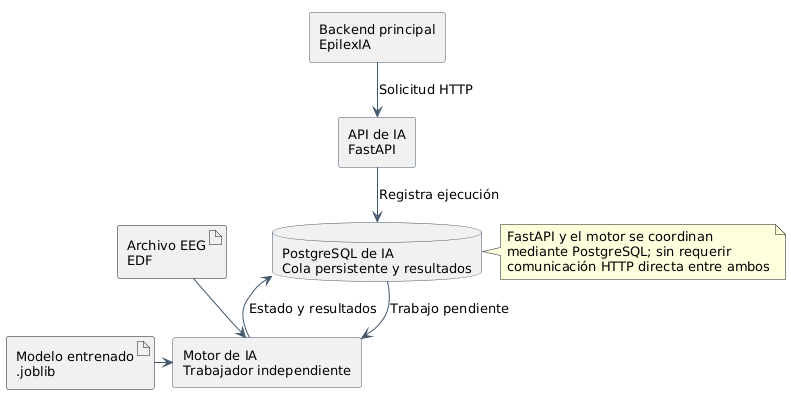
\includegraphics[width=\textwidth]{ThesisFigs/organizacion_procesamiento_ia_pgqueue.png}
    \caption{Organización del procesamiento de inteligencia artificial mediante cola persistente en EpilexIA.}
    \label{fig:organizacion-procesamiento-ia-pgqueue}
\end{figure}


\subsection{Preparación y procesamiento de señales EEG}
\label{subsec:preparacion-procesamiento-eeg-ia}

El procesamiento de señales electroencefalográficas mediante inteligencia artificial en EpilexIA parte de archivos digitales en formato EDF. El motor de inferencia accede al archivo asociado con la ejecución solicitada mediante una referencia a su ubicación en el almacenamiento, sin necesidad de transferir la totalidad de las muestras a través de la API de inteligencia artificial. Para interpretar el registro, el procedimiento utiliza la biblioteca MNE de Python.

El procedimiento de análisis forma parte del modelo de detección provisto por el equipo de ciencia de datos del proyecto, por lo que su diseño interno no integra el alcance del presente trabajo.
Para integrarlo, el motor considera sus etapas generales: la adaptación de las señales a un montaje bipolar longitudinal de 18 derivaciones, el remuestreo a 256~Hz, el filtrado, la segmentación en ventanas consecutivas de 10 segundos, la extracción de características de cada ventana y su normalización para cada registro.
La configuración de estas etapas se distribuye junto con el modelo entrenado, de modo que el motor aplica a cada estudio el mismo procedimiento con el que el modelo fue entrenado (Sección~\ref{subsec:modelo-vigente-hgb}).

El procesamiento se ejecuta de forma independiente de la navegación del especialista por la interfaz web. El trabajador obtiene las ejecuciones pendientes desde PostgreSQL, inicia el procedimiento de inferencia y actualiza la información de estado y resultados. Los intervalos temporales analizados se expresan en segundos relativos al inicio del registro, lo que permite relacionar las predicciones con las posiciones correspondientes dentro del estudio EEG.

Es importante distinguir este procedimiento del procesamiento realizado por el \textit{backend} principal para la visualización de señales. Mientras este último prepara segmentos destinados a la recuperación y navegación temporal del registro, el motor de inteligencia artificial construye características de las ventanas y aplica el modelo predictivo para identificar intervalos que podrían requerir revisión clínica.


\subsection{Generación e interpretación de resultados}
\label{subsec:generacion-interpretacion-resultados-ia}

Para cada ventana analizada, el modelo entrega una probabilidad de crisis.
Estos valores constituyen salidas del modelo y no deben interpretarse, por sí solos, como una confirmación clínica de actividad epiléptica.

La decisión de señalar un intervalo combina dos parámetros: un umbral de probabilidad y una cantidad mínima de ventanas consecutivas que deben superarlo.
Ambos se definen en el paquete del modelo.
Al registrarse una ejecución, el umbral aplicable se incorpora a sus datos, de manera que el valor utilizado permanece asociado al procesamiento correspondiente aunque la configuración se modifique posteriormente.
Los valores del modelo vigente se indican en la Sección~\ref{subsec:modelo-vigente-hgb}.

Durante el análisis, el motor genera un archivo temporal con la información de las ventanas procesadas y registra en PostgreSQL únicamente las que integran un intervalo señalado.

Cada resultado conservado se vincula con su ejecución de origen e incluye el tiempo de inicio y fin del intervalo, expresados en segundos respecto del comienzo del registro, así como la probabilidad de crisis utilizada para su selección. La relación con la ejecución permite recuperar el estudio asociado y la información necesaria para identificar el procesamiento que produjo el resultado. Las ventanas se registran individualmente, por lo que un intervalo señalado se presenta como una secuencia de registros consecutivos.

La finalización satisfactoria de una ejecución indica que el procedimiento concluyó conforme a su flujo operativo, pero no implica necesariamente la existencia de resultados positivos almacenados. Si ninguna ventana satisface los criterios de selección, el procesamiento puede finalizar con estado exitoso y sin registros de resultados. Asimismo, los estados de ejecución permiten diferenciar los trabajos pendientes o en curso de aquellos que finalizan, fallan, exceden el tiempo permitido o son cancelados.

En consecuencia, los intervalos generados por el subsistema de inteligencia artificial deben entenderse como indicaciones de posibles hallazgos que orientan la revisión del registro EEG. Su interpretación requiere considerar las señales originales y el contexto clínico del estudio. La decisión sobre la relevancia de cada intervalo corresponde al especialista, por lo que el componente automatizado cumple una función de apoyo y no sustituye la evaluación médica.


\subsection{Integración de resultados en la revisión clínica}
\label{subsec:integracion-resultados-revision-clinica}

La integración de los resultados de inteligencia artificial en EpilexIA tiene como propósito facilitar que el especialista examine los intervalos identificados durante el procesamiento automatizado en el contexto del estudio electroencefalográfico. Para ello, el sistema relaciona cada ejecución con el estudio clínico correspondiente y permite recuperar los resultados mediante los servicios de integración entre el \textit{backend} principal y la API de inteligencia artificial.

Una vez concluida la ejecución, el \textit{backend} principal puede consultar las ventanas que cumplen los criterios de detección y obtener sus límites temporales. Estos intervalos se expresan en segundos respecto del inicio del registro EEG, lo que permite relacionarlos con la posición correspondiente en las señales visualizadas. De este modo, los resultados automatizados funcionan como referencias temporales para orientar la inspección del registro, sin sustituir la observación directa de las señales.

La revisión clínica conserva una separación entre los resultados producidos por el modelo y las decisiones del especialista. La identificación automática de un intervalo no implica que este haya sido confirmado como un evento epiléptico. Su relevancia debe determinarse mediante el análisis de la actividad electroencefalográfica y de la información clínica disponible para el estudio.

El diseño contempla mecanismos para incorporar a los informes médicos las ventanas de inteligencia artificial seleccionadas durante la revisión. La asociación conserva la referencia a la ejecución y al resultado de origen, así como información descriptiva y de clasificación aportada por el profesional. Esta vinculación permite distinguir los intervalos identificados automáticamente de aquellos que el especialista decide utilizar como parte de su informe.

Asimismo, EpilexIA permite registrar anomalías y anotaciones definidas manualmente por el especialista, incluso cuando no corresponden a una ventana previamente detectada por el modelo. Las anotaciones manuales y las ventanas de inteligencia artificial incluidas en un informe se gestionan como conjuntos diferenciados y pueden sincronizarse con el subsistema de IA mediante interfaces específicas. Por consiguiente, la ausencia de una detección automática no impide que el profesional documente un hallazgo observado durante la revisión.

La información de retroalimentación clínica se conserva en estructuras específicas del subsistema de inteligencia artificial. En particular, las inclusiones de ventanas en informes permiten mantener su asociación con la revisión profesional, mientras que las anotaciones manuales registran observaciones originadas en la evaluación del especialista. Estos datos podrían servir como insumos para procesos posteriores de mejora de los modelos, pero su almacenamiento no implica que EpilexIA ejecute automáticamente un reentrenamiento.

La organización de los informes mantiene la responsabilidad de cada especialista sobre el contenido clínico que elabora. Así, la consulta de resultados automatizados y la selección de ventanas para un informe se integran al flujo de trabajo médico sin convertir las predicciones en conclusiones diagnósticas obligatorias. La interpretación final y la elaboración del informe corresponden al profesional responsable.

En síntesis, la integración de resultados vincula las ejecuciones de inteligencia artificial con la navegación temporal del EEG, la documentación de hallazgos y la elaboración de informes clínicos. El componente automatizado aporta referencias para la revisión, mientras que la valoración de su significado clínico permanece bajo el criterio del especialista.


\section{Diseño de seguridad y control de acceso}
\label{sec:seguridad-control-acceso}

El diseño de seguridad de EpilexIA contempla mecanismos destinados a controlar el acceso a las funcionalidades del sistema y a la información asociada con los pacientes, los estudios electroencefalográficos y los informes clínicos. Dada la naturaleza de estos datos, el acceso se organiza mediante la identificación de los usuarios, la asignación de permisos y la verificación de las condiciones necesarias para realizar cada operación.

La autenticación se realiza a través del \textit{backend} principal, que emite un \textit{token} de acceso para las sesiones válidas. Las solicitudes posteriores a los servicios protegidos incorporan dicho \textit{token}, cuya validez se comprueba antes de permitir el procesamiento de la operación. Este mecanismo se complementa con el registro de sesiones, lo que permite controlar la vigencia de los accesos autenticados.

La autorización combina permisos asociados a los roles del sistema con verificaciones adicionales sobre los recursos clínicos. Por ello, disponer de un permiso general para consultar o modificar estudios no implica necesariamente poder acceder a cualquier registro: determinadas operaciones también dependen de la relación del usuario con el estudio o el informe correspondiente.

En la aplicación web, las rutas y acciones disponibles se presentan de acuerdo con la autenticación y los permisos del usuario. Sin embargo, estas restricciones de interfaz no sustituyen las verificaciones realizadas por el \textit{backend}, que constituye el punto de control para autorizar las solicitudes recibidas.

Los siguientes apartados describen los mecanismos de autenticación, la organización de roles y permisos, las reglas de acceso a recursos clínicos y las consideraciones de protección de datos y comunicaciones contempladas en el diseño de EpilexIA.


\subsection{Autenticación de usuarios}
\label{subsec:autenticacion-usuarios}

La autenticación de usuarios en EpilexIA se realiza a través del \textit{backend} principal y constituye el mecanismo de identificación previo al acceso a los servicios protegidos. El proceso comienza cuando el usuario introduce sus credenciales en la interfaz web. Estas se remiten al servicio de autenticación, que comprueba su validez y las condiciones de acceso de la cuenta antes de establecer una sesión.

Cuando las credenciales son válidas, el \textit{backend} genera un \textit{token} de acceso en formato \textit{JSON Web Token} (JWT).
 El \textit{token} se firma digitalmente e incorpora información que permite identificar al usuario y determinar su período de vigencia. Asimismo, contiene un identificador único de \textit{token}, denominado \texttt{jti}, que se utiliza para relacionarlo con un registro de sesión persistido en la base de datos clínica. La respuesta de autenticación proporciona al \textit{frontend} la información necesaria para continuar las operaciones del usuario, incluidos sus permisos.

En las solicitudes posteriores, la aplicación web incorpora el \textit{token} mediante el encabezado HTTP \texttt{Authorization}, utilizando el esquema \texttt{Bearer}. Antes de permitir el acceso a los servicios protegidos, el \textit{backend} comprueba la firma y la expiración del JWT, extrae su identificador \texttt{jti} y verifica que exista una sesión vigente asociada. Si alguna de estas condiciones no se cumple, la solicitud no se considera autenticada.

La configuración de seguridad utiliza una política de procesamiento HTTP sin estado, denominada \texttt{stateless}. Esto significa que la autenticación no depende de una sesión HTTP tradicional mantenida entre solicitudes. No obstante, EpilexIA conserva registros de sesiones de usuario en la base de datos, lo que permite controlar la vigencia de los \textit{tokens} emitidos y revocarlos antes de que alcancen su fecha de expiración.

Una vez validado el \textit{token}, el \textit{backend} recupera la información actual del usuario y las autoridades correspondientes a sus permisos. De esta manera, la autenticación establece la identidad del solicitante, mientras que la autorización posterior determina qué operaciones puede realizar. La validación de un JWT, por sí sola, no concede acceso indiscriminado a los recursos clínicos del sistema.

El cierre de sesión dispone de una operación específica que identifica el \textit{token} utilizado y elimina el registro de sesión correspondiente. En consecuencia, aunque el JWT conserve una firma válida y no haya alcanzado su expiración, deja de ser aceptado cuando ya no existe una sesión vigente asociada a su identificador. Asimismo, el procedimiento de restablecimiento de contraseña contempla la invalidación de sesiones para impedir la continuidad de accesos previamente autorizados.

El diseño también contempla procedimientos de activación de cuentas y restablecimiento de contraseñas mediante \textit{tokens} específicos, distintos de los JWT utilizados para acceder a los servicios clínicos. Estos mecanismos permiten gestionar el establecimiento o la recuperación de credenciales sin confundir dichas operaciones con una sesión autenticada de uso ordinario.

En conjunto, la autenticación de EpilexIA combina la verificación de credenciales, la emisión de \textit{tokens} firmados y el control de sesiones persistidas. Esta organización proporciona una base para identificar a los usuarios y aplicar posteriormente las reglas de roles, permisos y acceso contextual a los recursos clínicos, desarrolladas en los siguientes apartados.


\subsection{Roles y permisos}
\label{subsec:roles-permisos}

El control de acceso de EpilexIA se organiza mediante un esquema de autorización basado en roles y permisos. Cada usuario dispone de un rol asociado con un conjunto de operaciones autorizadas, de acuerdo con las responsabilidades que desempeña dentro del sistema. Esta organización permite diferenciar las funciones administrativas, el registro y la preparación de estudios, y las actividades de revisión clínica.

El modelo vigente contempla tres roles: Administrador, Técnico y Especialista. El Administrador se orienta a la gestión de usuarios, roles y permisos, además de las operaciones de supervisión y administración disponibles en el sistema. El Técnico participa principalmente en el registro de pacientes y estudios electroencefalográficos, así como en la incorporación de los archivos correspondientes. El Especialista desarrolla las tareas clínicas de consulta y revisión de estudios, análisis de señales, registro de hallazgos y elaboración de informes médicos.

El Cuadro~\ref{tab:roles-permisos-epilexia} resume las responsabilidades principales de estos perfiles. Se trata de una descripción funcional de los roles, no de una enumeración exhaustiva de todas las autorizaciones almacenadas en la base de datos.

\begin{table}[H]
\centering
\caption{Responsabilidades principales de los roles de EpilexIA.}
\label{tab:roles-permisos-epilexia}
\small
\begin{tabular}{|p{0.20\textwidth}|p{0.68\textwidth}|}
\hline
\textbf{Rol} & \textbf{Responsabilidades principales} \\ \hline
Administrador & Gestión de usuarios, roles y permisos; acceso administrativo y supervisión de los recursos del sistema conforme a las autorizaciones disponibles. \\ \hline
Técnico & Registro y actualización de información de pacientes, creación de estudios EEG e incorporación de archivos asociados a los estudios en los que participa. \\ \hline
Especialista & Consulta y revisión de estudios EEG, análisis de señales, registro de anomalías y eventos, y creación y gestión de informes clínicos conforme a los permisos y reglas de acceso aplicables. \\ \hline
\end{tabular}
\end{table}

Los permisos se representan mediante identificadores asociados a recursos y acciones. Por ejemplo, \texttt{patients.list}, \texttt{studies.create}, \texttt{reports.update} y \texttt{anomalies.create} expresan autorizaciones para consultar pacientes, registrar estudios, actualizar informes y crear anomalías, respectivamente. Esta separación permite controlar operaciones concretas sin depender exclusivamente del nombre del rol.

La relación entre roles y permisos se mantiene en la base de datos clínica. Al autenticarse, el usuario recibe información sobre sus permisos, que la aplicación web utiliza para habilitar rutas y presentar las acciones correspondientes. En el \textit{backend}, los permisos se traducen en autoridades de seguridad y se verifican en los servicios protegidos antes de ejecutar las operaciones solicitadas.

La asignación de permisos puede administrarse mediante las funcionalidades destinadas a la gestión de roles. Por ello, el conjunto de acciones disponible para un usuario depende de las autorizaciones efectivamente asociadas a su rol, y no únicamente de la denominación de este. Las asignaciones iniciales previstas en los scripts de base de datos constituyen una configuración de referencia que puede diferir de la existente en una instalación administrada.

Es importante distinguir los permisos funcionales de las condiciones de acceso a un registro particular. Por ejemplo, disponer de autorización para consultar estudios no implica necesariamente poder visualizar cualquier estudio EEG. El sistema aplica comprobaciones adicionales según la participación del usuario y su relación con el recurso solicitado. Estas reglas de autorización contextual se desarrollan en el apartado siguiente.

De esta manera, la organización por roles y permisos proporciona un mecanismo para distribuir responsabilidades y restringir las operaciones disponibles, mientras que las verificaciones específicas sobre pacientes, estudios e informes complementan el control de acceso a la información clínica.


\subsection{Autorización sobre recursos clínicos}
\label{subsec:autorizacion-recursos-clinicos}

La autorización sobre recursos clínicos en EpilexIA complementa los permisos asociados a los roles mediante verificaciones relacionadas con el registro solicitado. Este mecanismo permite distinguir entre disponer de autorización para ejecutar una operación y estar habilitado para realizarla sobre un paciente, estudio electroencefalográfico o informe determinado. Las comprobaciones se efectúan en el \textit{backend} principal, de manera que la presentación de acciones en la interfaz web no constituye por sí sola una autorización suficiente.

En los servicios vinculados a estudios EEG, el control de acceso considera la relación del usuario con cada estudio. La consulta se permite al Administrador, al Técnico que registró el estudio, al Especialista responsable y a los especialistas incorporados como observadores, siempre que dispongan también de los permisos funcionales requeridos. Por el contrario, un Especialista que no mantiene una relación autorizada con el estudio no adquiere acceso únicamente por pertenecer al mismo rol clínico.

Las operaciones de modificación de los datos del estudio están sujetas a condiciones más restrictivas. De acuerdo con las reglas de acceso implementadas, estas operaciones se habilitan al Administrador o al Especialista responsable, según los permisos correspondientes. La condición de observador permite participar en la revisión del estudio, pero no otorga por sí misma autorización para modificar sus datos generales. Asimismo, el Técnico que registró el estudio no adquiere por ese hecho las facultades de modificación reservadas a otros participantes.

La incorporación de archivos asociados al estudio utiliza una comprobación específica. Además del permiso requerido para la operación, pueden realizar la carga el Administrador, el Especialista responsable y el Técnico creador del estudio. Esta capacidad se encuentra condicionada por el estado del registro: los estudios anulados no admiten nuevas cargas. De esta manera, la autorización considera tanto la relación del usuario con el estudio como las condiciones de la operación solicitada.

En el visualizador EEG, el acceso a señales, segmentos y otros recursos del estudio se apoya en las reglas de consulta previamente descritas. Por su parte, el registro y la modificación de anomalías y eventos EEG requieren permisos específicos y verificaciones adicionales sobre la participación del usuario. Esta separación evita equiparar la capacidad de observar las señales con la autorización para modificar los hallazgos asociados al estudio.

La gestión de informes médicos incorpora un control adicional basado en la autoría. EpilexIA permite que distintos especialistas vinculados a un mismo estudio elaboren informes propios. La relación entre el estudio, el informe y su autor se conserva en los registros correspondientes, y el sistema establece que cada especialista puede disponer de un único informe propio por estudio. Por tanto, tanto el Especialista responsable como los Especialistas incorporados como observadores autorizados pueden elaborar sus propios informes médicos asociados al estudio, siempre que dispongan de los permisos correspondientes. Cada informe pertenece al Especialista que lo creó y no puede ser modificado por otros profesionales.


La consulta de un informe perteneciente a otro profesional no implica autorización para modificarlo. Cuando un especialista accede a un informe ajeno mediante los servicios vinculados al estudio, la información se presenta en modo de solo lectura. La edición del informe propio requiere, además de los permisos funcionales, que se cumplan las condiciones relativas a su autoría y estado. La creación de nuevos informes también está condicionada por las reglas del proceso, entre ellas la inexistencia de un informe propio previo y las restricciones asociadas al cierre de informes del estudio.

En cuanto a los datos de pacientes, la autorización se organiza principalmente mediante permisos funcionales de consulta, creación y actualización. A diferencia de las comprobaciones contextuales aplicadas a los estudios, las operaciones generales sobre pacientes no se restringen al Técnico creador ni al Especialista asignado: dependen únicamente de los permisos del usuario. Esta distinción es relevante para describir con precisión el alcance de las verificaciones presentes en cada servicio.

Finalmente, las reglas de acceso contextual se aplican en los servicios que incorporan expresamente dichas comprobaciones. Algunas operaciones generales de búsqueda y exportación utilizan controles basados en permisos sin reproducir necesariamente todas las restricciones de participación de los servicios asociados a un estudio particular. Por ello, el diseño de seguridad debe analizarse considerando conjuntamente las autoridades exigidas por cada interfaz y las verificaciones adicionales realizadas por su lógica de aplicación.

En síntesis, la autorización sobre recursos clínicos combina permisos funcionales, relaciones de participación y condiciones propias de los registros. Esta organización permite diferenciar la consulta de estudios, la modificación de datos, la incorporación de archivos y la gestión de informes, manteniendo la responsabilidad de las decisiones clínicas en los especialistas habilitados.


\subsection{Protección de datos y comunicaciones}
\label{subsec:proteccion-datos-comunicaciones}

La protección de la información en EpilexIA comprende tanto los datos clínicos almacenados como las comunicaciones entre los componentes de la plataforma. Debido a que el sistema gestiona información de pacientes, registros electroencefalográficos, archivos de video e informes médicos, su diseño combina controles de acceso de aplicación con mecanismos de separación de servicios y medidas que deben completarse en el entorno de despliegue.

En el tratamiento de las credenciales, el sistema distingue las contraseñas utilizadas para autenticar a los usuarios de los \textit{tokens} de acceso emitidos para las sesiones. La creación y recuperación de cuentas se realizan mediante procedimientos específicos de activación y restablecimiento de contraseña. Por su parte, las solicitudes autenticadas utilizan \textit{tokens} JWT, cuya validación y revocación se describieron en el apartado~\ref{subsec:autenticacion-usuarios}. Estos mecanismos evitan que la autorización de las operaciones clínicas dependa únicamente de los controles visibles en la interfaz web.

La comunicación habitual comienza en el navegador y pasa por el servidor web Nginx, que entrega la aplicación y encamina las solicitudes hacia el \textit{backend} principal. Este último centraliza la autenticación, la autorización y el acceso a los recursos clínicos. La comunicación con el subsistema de inteligencia artificial se realiza mediante una interfaz de servicio diferenciada, que utiliza autenticación HTTP Basic con credenciales configuradas para la integración. En consecuencia, las credenciales del usuario clínico y las empleadas entre servicios cumplen funciones distintas.

El cifrado de las comunicaciones constituye una consideración específica del despliegue. El uso de HTTPS con TLS permite proteger la información transmitida entre el navegador y el punto de entrada del sistema frente a su lectura o alteración durante el transporte. En el entorno de despliegue utilizado, el acceso de los usuarios se realiza mediante HTTPS (Sección~\ref{subsec:despliegue-nube}), mientras que los servicios internos se comunican dentro de la red del propio entorno. La habilitación de HTTPS y la configuración de los certificados forman parte de la instalación en cada infraestructura donde se despliegue EpilexIA.

Los datos estructurados se conservan en bases PostgreSQL diferenciadas: una destinada a los registros clínicos y otra a las ejecuciones y resultados del subsistema de inteligencia artificial. Los archivos EEG y de video se mantienen en almacenamiento persistente separado de las tablas relacionales. De igual manera, los artefactos de los modelos de aprendizaje automático se alojan en recursos de archivos accesibles para los componentes que ejecutan las inferencias. Esta distribución permite administrar por separado los registros, los archivos de gran tamaño y los modelos utilizados.

La persistencia de estos recursos requiere medidas operativas adicionales. El diseño de despliegue mediante contenedores y volúmenes permite conservar la información aunque se detengan o reinicien los servicios, pero no reemplaza la necesidad de realizar copias de seguridad. Los recursos críticos del sistema son el almacenamiento de EEG y video, la base clínica y la base de inteligencia artificial, cuya conservación y respaldo deben contemplarse en la administración de la infraestructura.

La configuración de los servicios también incluye información sensible, como las credenciales de conexión a las bases de datos, la clave utilizada para firmar JWT y las credenciales de integración con la API de inteligencia artificial. Estos valores deben gestionarse en el entorno de operación y no incorporarse al contenido público de la aplicación web ni a la documentación distribuida. La protección efectiva de tales parámetros depende asimismo de las restricciones de acceso al servidor y a su configuración.

En cuanto al seguimiento técnico, EpilexIA dispone de mecanismos de registro que permiten relacionar solicitudes y operaciones mediante identificadores de trazabilidad. Las contraseñas y los \textit{tokens} se enmascaran en los registros estructurados. No obstante, la disponibilidad de estos registros no sustituye la aplicación de controles de acceso a los propios archivos de auditoría ni las políticas de conservación de información clínica.

En síntesis, el diseño de protección de datos y comunicaciones combina autenticación, autorización, separación de componentes, almacenamiento persistente y trazabilidad de operaciones. Su efectividad requiere complementar los controles implementados en la aplicación con una configuración segura de red, cifrado de transporte, gestión de credenciales y procedimientos de respaldo adecuados al entorno institucional de operación.

\section{Diseño de auditoría y trazabilidad}
\label{sec:diseno-auditoria-trazabilidad}

El diseño de auditoría y trazabilidad de EpilexIA contempla mecanismos para registrar operaciones relevantes del sistema y facilitar el seguimiento de las actividades realizadas sobre sus recursos. Dado que la plataforma administra información de pacientes, estudios electroencefalográficos e informes clínicos, resulta necesario disponer de registros que permitan reconocer las acciones efectuadas y el contexto en el que se produjeron.

La auditoría funcional se apoya en eventos persistidos en la base de datos clínica. Estos registros permiten identificar operaciones de negocio seleccionadas y conservar información sobre el actor, la acción realizada y los datos de contexto correspondientes. Su consulta proporciona una visión histórica de las actividades registradas, sin que ello implique que todas las solicitudes HTTP o todos los cambios internos generen necesariamente un evento de auditoría persistente.

Para facilitar la revisión de esta información, EpilexIA incorpora una vista de actividad reciente en el panel principal y una interfaz de consulta de auditorías. Esta última permite explorar los registros mediante paginación, ordenamiento cronológico y filtros combinables, de acuerdo con las autorizaciones exigidas por los servicios del \textit{backend}.

De manera complementaria, los componentes de aplicación producen registros técnicos que permiten seguir solicitudes y diagnosticar incidencias. Estos registros utilizan identificadores de trazabilidad para relacionar las etapas de una operación. En el subsistema de inteligencia artificial, el identificador de ejecución permite además vincular el seguimiento técnico con los estados y resultados del procesamiento asíncrono.

Por tanto, el diseño distingue entre los eventos de auditoría conservados para la consulta funcional y los registros técnicos utilizados para el seguimiento operativo. Los siguientes apartados describen el registro de operaciones y eventos, los mecanismos de consulta de auditorías y la trazabilidad de procesos e integraciones entre componentes.


\subsection{Registro de operaciones y eventos}
\label{subsec:registro-operaciones-eventos}

El registro de operaciones y eventos en EpilexIA tiene como finalidad conservar información sobre determinadas actividades realizadas dentro del sistema, permitiendo identificar las acciones ejecutadas y el contexto en el que se produjeron. Este mecanismo constituye una parte de la auditoría funcional y proporciona información para la revisión posterior de las operaciones relacionadas con los recursos administrados por la plataforma.

La implementación de auditoría se encuentra integrada en el \textit{backend}
principal. Para identificar las operaciones de negocio que generan
eventos de auditoría persistentes, el sistema utiliza la enumeración
\texttt{AuditEventType}. Estos eventos son publicados por los servicios
de aplicación y procesados mediante componentes específicos que
permiten conservarlos en la base de datos clínica.

De manera complementaria, el \textit{backend} utiliza la enumeración
\texttt{LogAction} para identificar operaciones registradas mediante
el mecanismo de \textit{logging} estructurado. Este mecanismo proporciona
trazas técnicas para el seguimiento de solicitudes y operaciones,
pero no implica necesariamente la generación de un evento de
auditoría persistente.

El registro de auditoría contempla operaciones relacionadas con la administración del sistema y la gestión de sus recursos. Entre ellas se encuentran determinadas acciones sobre usuarios, pacientes, estudios electroencefalográficos e informes médicos. La generación de estos registros depende de los puntos de la aplicación en los que se encuentra incorporado el mecanismo de auditoría, por lo que no debe interpretarse como un registro automático y exhaustivo de todas las solicitudes recibidas por el \textit{backend}.

Para conservar la información de los eventos, EpilexIA utiliza estructuras persistentes en la base de datos clínica PostgreSQL. Los registros de auditoría permiten asociar una operación con información contextual, como el usuario que la realizó, la acción registrada y el momento en que ocurrió. Según el tipo de evento, también pueden incorporarse referencias a los recursos involucrados y otros datos necesarios para describir la actividad.

La implementación incorpora componentes específicos para intervenir en el registro de eventos, entre ellos \texttt{AuditEventRecordListener}. Este componente forma parte del mecanismo utilizado por el \textit{backend} para gestionar la información de auditoría. Su participación debe distinguirse de los registros técnicos generales, ya que estos últimos están destinados principalmente al diagnóstico y seguimiento operativo de los servicios.

La conservación de eventos en la base de datos permite consultar posteriormente las actividades registradas sin depender exclusivamente de los mensajes producidos durante la ejecución de la aplicación. Esta persistencia facilita la construcción de vistas de actividad y servicios de consulta que recuperan los registros conforme a los criterios solicitados.

Es importante señalar que la existencia de un registro de auditoría no implica necesariamente que se conserve una copia completa del contenido anterior y posterior de cada recurso modificado. El alcance de la información disponible depende de los datos registrados para cada operación. Por esta razón, los eventos deben interpretarse como evidencias de actividades específicas y no como un mecanismo general de reconstrucción de todos los estados históricos del sistema.

Asimismo, el registro de una operación no sustituye las verificaciones de autenticación y autorización. Los controles de acceso determinan si una solicitud puede ejecutarse, mientras que la auditoría permite conservar información sobre las actividades para las cuales se ha previsto su registro. Ambos mecanismos cumplen funciones complementarias dentro del diseño de seguridad de EpilexIA.

En conjunto, el registro de operaciones y eventos proporciona una base persistente para el seguimiento de las actividades relevantes del sistema. Su integración con los servicios de consulta permite que los usuarios autorizados examinen posteriormente los eventos almacenados, identifiquen las operaciones registradas y dispongan de información contextual para su revisión.


\subsection{Consulta y seguimiento de auditorías}
\label{subsec:consulta-seguimiento-auditorias}

La consulta de auditorías en EpilexIA permite recuperar y examinar las operaciones registradas por el sistema, proporcionando información sobre las actividades realizadas y su contexto. Esta funcionalidad complementa el mecanismo de registro de eventos descrito anteriormente y facilita la revisión de las acciones ejecutadas sobre los recursos de la plataforma.

El sistema dispone de una vista de actividad reciente integrada en el panel principal, destinada a presentar un resumen de las operaciones registradas. Esta visualización permite identificar acontecimientos recientes sin necesidad de acceder inicialmente a la consulta completa de auditorías.


La Figura~\ref{fig:actividad-reciente} ilustra esta funcionalidad mediante una lista de operaciones registradas, acompañadas de sus respectivas fechas y horas. Asimismo, se observa el acceso a la consulta completa de auditorías.

\begin{figure}[H]
    \centering
    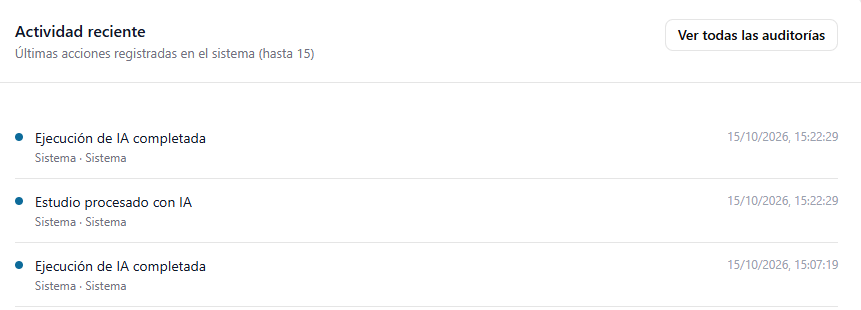
\includegraphics[width=0.90\textwidth]{ThesisFigs/actividad_reciente_epilexia.png}
    \caption{Vista de actividad reciente en el panel principal de EpilexIA.}
    \label{fig:actividad-reciente}
\end{figure}


Para una revisión más detallada, EpilexIA incorpora la interfaz denominada ``Ver todas las auditorías'', que permite consultar los registros mediante una tabla organizada. Esta interfaz presenta información de las operaciones registradas, incluyendo datos relacionados con el usuario, su rol, la acción realizada y la fecha del evento, según los atributos disponibles en cada registro.

La consulta contempla mecanismos de filtrado que permiten restringir los resultados conforme a diferentes criterios. Entre ellos se encuentran la búsqueda por usuario, la selección de roles y acciones, y la delimitación de fechas. La combinación de estos filtros facilita la localización de actividades específicas dentro del conjunto de registros disponibles.


En particular, el filtrado por fecha utiliza un control de selección que permite indicar el día de interés, mientras que la selección de roles se realiza mediante las opciones disponibles en el sistema. Estos controles reducen la necesidad de introducir manualmente determinados valores y contribuyen a mantener criterios de búsqueda consistentes.

Los resultados se presentan mediante paginación, de manera que la interfaz recupera y muestra una cantidad limitada de registros por página. Este mecanismo evita presentar simultáneamente la totalidad de los eventos almacenados y facilita la navegación entre los resultados de una consulta. Asimismo, el ordenamiento permite organizar los registros conforme a los criterios admitidos por el servicio, incluyendo su secuencia temporal.


La Figura~\ref{fig:consulta-auditorias} presenta
la interfaz de consulta de auditorías de EpilexIA.
En ella se observan los registros de actividad
organizados por fecha y hora, evento, actor,
rol y contexto, junto con los controles de
filtrado y paginación disponibles.


\begin{figure}[H]
    \centering
    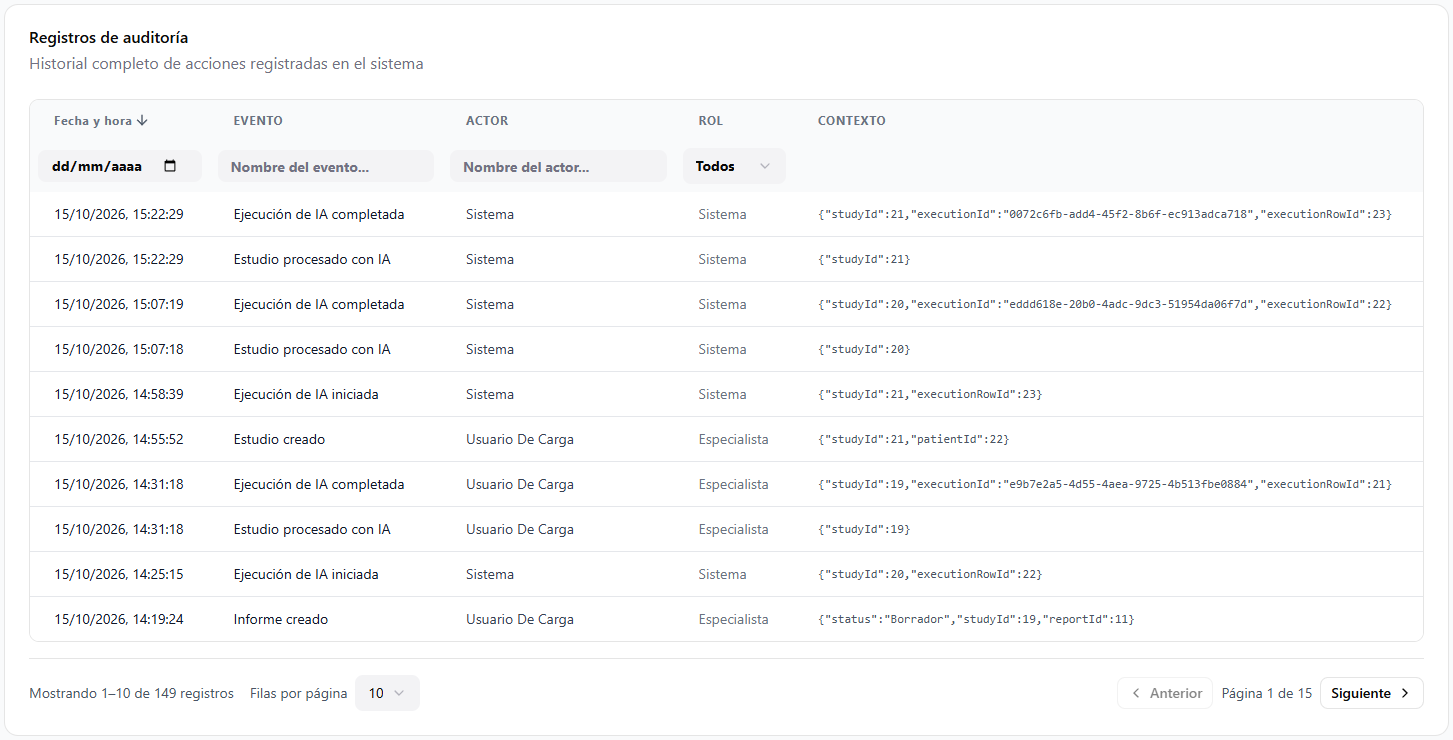
\includegraphics[width=\textwidth]{ThesisFigs/consulta_auditorias_epilexia.png}
    \caption{Consulta, filtrado y paginación de auditorías en EpilexIA.}
    \label{fig:consulta-auditorias}
\end{figure}


La recuperación de la información se realiza mediante servicios REST del \textit{backend} principal. Estos servicios reciben los parámetros de búsqueda y paginación, consultan los registros disponibles y devuelven los resultados correspondientes a la aplicación web. El procesamiento de los criterios de consulta en el servidor permite mantener una separación entre la presentación de los datos y la lógica encargada de recuperarlos.

El acceso a las funcionalidades de auditoría se encuentra sujeto a los permisos definidos para los usuarios del sistema. La interfaz web presenta las opciones correspondientes a las autorizaciones disponibles, mientras que el \textit{backend} verifica los permisos requeridos antes de responder a las solicitudes de consulta.

Es importante señalar que la información presentada corresponde a los eventos efectivamente registrados por los mecanismos de auditoría de EpilexIA. Por consiguiente, la ausencia de una actividad en los resultados de búsqueda no demuestra, por sí sola, que ninguna operación relacionada haya ocurrido, dado que el alcance del registro depende de los eventos contemplados por la aplicación.

En conjunto, la consulta y el seguimiento de auditorías proporcionan herramientas para examinar las actividades registradas, localizar operaciones mediante filtros y navegar por los resultados de manera organizada. Estas funcionalidades contribuyen a la supervisión administrativa y complementan los mecanismos de seguridad y trazabilidad del sistema.

% FIGURA OPCIONAL: activar después de subir la imagen a ThesisFigs.
% La Figura~\ref{fig:consulta-auditorias-epilexia} presenta la interfaz de consulta de auditorías.
% \begin{figure}[H]
%     \centering
%     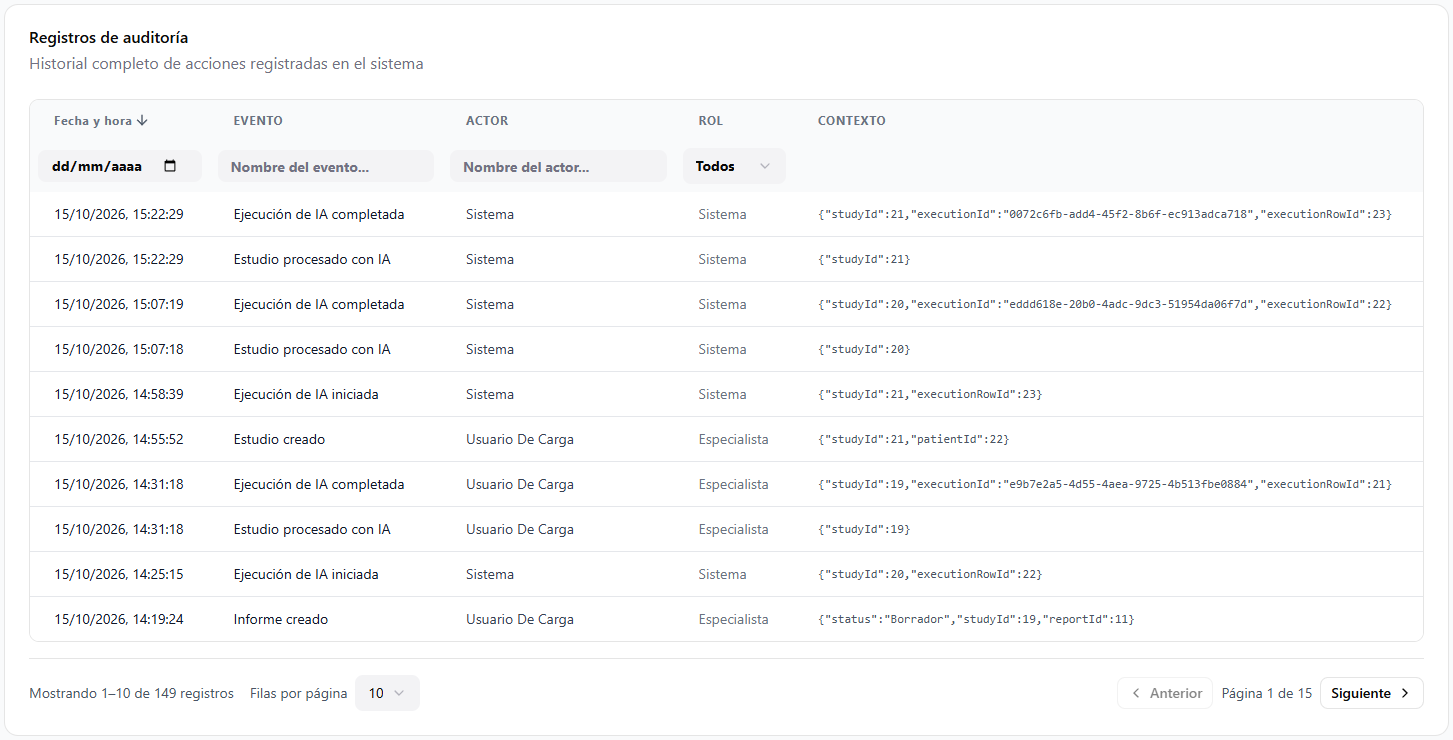
\includegraphics[width=\textwidth]{ThesisFigs/consulta_auditorias_epilexia.png}
%     \caption{Interfaz de consulta y filtrado de auditorías del sistema EpilexIA.}
%     \label{fig:consulta-auditorias-epilexia}
% \end{figure}


\subsection{Trazabilidad de procesos e integración}
\label{subsec:trazabilidad-procesos-integracion}

La trazabilidad de procesos en EpilexIA comprende los mecanismos
que permiten relacionar las solicitudes recibidas por los
servicios de aplicación con las operaciones ejecutadas por
sus distintos componentes. Esta capacidad resulta especialmente
relevante en los procedimientos que involucran varias etapas
de procesamiento o requieren comunicación entre servicios
independientes.

En el \textit{backend} principal, los registros técnicos permiten
conservar información sobre el procesamiento de solicitudes
y las incidencias que pueden producirse durante su ejecución.
Para facilitar su seguimiento, se utilizan identificadores
de trazabilidad que permiten relacionar los mensajes
correspondientes a una misma operación. Estos registros
cumplen una función operativa y deben distinguirse de los
eventos de auditoría funcional almacenados en la base de
datos clínica.

La integración con el subsistema de inteligencia artificial
incorpora un mecanismo adicional de identificación. Cada
solicitud de procesamiento aceptada se asocia con un
identificador de ejecución, denominado
\texttt{executionId}, que permite reconocer el trabajo
correspondiente durante las distintas etapas de su ciclo
de vida. Este identificador constituye una referencia
para consultar el estado del procesamiento y recuperar
los resultados generados.

La API de inteligencia artificial registra la ejecución
en su base de datos PostgreSQL. Posteriormente, el motor
independiente obtiene los trabajos pendientes, realiza
el procesamiento de las señales EEG y actualiza la
información correspondiente a sus estados y resultados.
La persistencia de estos registros permite seguir
el avance del trabajo sin depender de una conexión
HTTP continua entre la API y el motor. La organización
de estos componentes y su mecanismo de coordinación
mediante PostgreSQL se ilustran en la
Figura~\ref{fig:organizacion-procesamiento-ia-pgqueue}.


El seguimiento de las ejecuciones contempla estados
que permiten diferenciar los trabajos pendientes,
aquellos que se encuentran en procesamiento y los
que han finalizado. Asimismo, se consideran situaciones
de fallo, cancelación o superación del tiempo permitido.
Esta información permite distinguir entre la aceptación
inicial de una solicitud y la finalización efectiva
del análisis automatizado.

La relación entre los componentes también se apoya
en los identificadores de los estudios clínicos.
El \textit{backend} principal conserva la información del
estudio EEG, mientras que el subsistema de inteligencia
artificial registra las ejecuciones y los resultados
asociados mediante referencias lógicas. Dado que
ambos subsistemas utilizan bases de datos independientes,
estas referencias permiten establecer la correspondencia
entre sus registros sin requerir claves foráneas
entre las dos bases de datos.

Los resultados del procesamiento mantienen su
asociación con la ejecución que los produjo. De esta
manera, es posible identificar el análisis de origen
de los intervalos detectados y relacionarlos con el
estudio electroencefalográfico correspondiente. Esta
vinculación facilita la recuperación de información
desde los servicios de integración y su presentación
durante la revisión clínica.

De forma complementaria, los eventos de auditoría
funcional permiten conservar determinadas acciones
relacionadas con el inicio y la finalización de
procesamientos de inteligencia artificial, cuando
estas operaciones se encuentran contempladas por
los mecanismos de registro del \textit{backend}. Su finalidad
es documentar actividades relevantes para la consulta
posterior, mientras que los estados de ejecución y
los registros técnicos proporcionan información
más específica para el seguimiento operativo.

Es importante señalar que estos mecanismos no
constituyen necesariamente una traza única y completa
de todas las operaciones realizadas por los componentes.
El nivel de detalle disponible depende de los
identificadores propagados, los registros generados
por cada servicio y los eventos efectivamente
persistidos durante el procesamiento.

En conjunto, la trazabilidad de procesos e integración
de EpilexIA combina identificadores de solicitudes,
referencias a estudios clínicos, identificadores de
ejecución y registros de estado. Esta organización
facilita el seguimiento de los procedimientos
distribuidos, la identificación de incidencias y
la relación entre las operaciones técnicas y los
recursos clínicos involucrados.


\section{Diseño de interfaz de usuario}
\label{sec:diseno-interfaz-usuario}

El diseño de la interfaz de usuario de EpilexIA se orienta a facilitar la interacción de los distintos perfiles con las funcionalidades del sistema. Para ello, considera las necesidades de administración, de registro y gestión de estudios electroencefalográficos, de identificación de pacientes durante la creación de estudios y de revisión clínica.

La organización de la interfaz contempla los tres
roles definidos en el sistema: Administrador, Técnico
y Especialista. Cada perfil dispone de opciones de
navegación y acciones relacionadas con sus permisos,
de manera que las funcionalidades presentadas
correspondan a las tareas que puede desempeñar.
Esta diferenciación contribuye a organizar el acceso
a los recursos y a reducir la exposición de opciones
que no forman parte de las responsabilidades del
usuario.

La aplicación web se desarrolla mediante React y
utiliza componentes reutilizables para estructurar
las pantallas, los formularios, las tablas de datos
y los controles de interacción. Su diseño contempla
la adaptación de los elementos visuales a diferentes
dimensiones de pantalla, procurando mantener una
distribución adecuada de la información y facilitar
la navegación entre las funcionalidades disponibles.

Una parte central del diseño corresponde a la
visualización de estudios EEG. Debido a la naturaleza
temporal de las señales electroencefalográficas,
esta interfaz incorpora mecanismos de navegación
por el registro, selección de montajes, ajuste de
filtros y sensibilidad, así como opciones para ampliar
el área de visualización. Estos controles permiten
al especialista examinar las señales y relacionarlas
con los eventos y hallazgos asociados al estudio.


El diseño también contempla la presentación de los resultados de inteligencia artificial disponibles para cada estudio. Los intervalos registrados se integran en el entorno de revisión clínica como información complementaria, permitiendo al Especialista consultar las señales correspondientes y determinar su relevancia. Asimismo, la interfaz facilita el registro de anomalías, eventos y la elaboración de informes médicos vinculados al estudio.


En las operaciones de administración y gestión,
la interfaz utiliza formularios, tablas y mecanismos
de búsqueda para facilitar la consulta y actualización
de la información. Estas funcionalidades se complementan
con mensajes de estado y controles de interacción
que permiten comunicar al usuario el resultado de
las operaciones realizadas.

Los siguientes apartados describen la organización
general de la interfaz, las pantallas destinadas
a la administración y gestión de estudios, el
visualizador EEG y los componentes utilizados
para la revisión clínica y elaboración de informes.


\subsection{Organización general de la interfaz}
\label{subsec:organizacion-general-interfaz}

La interfaz web de EpilexIA se organiza mediante
pantallas destinadas a las principales actividades
del sistema. Su estructura permite que los usuarios
accedan a las funcionalidades correspondientes a
su perfil y mantengan una navegación consistente
entre las operaciones de administración, gestión
de estudios y revisión clínica.

El acceso a la aplicación comienza con una pantalla
de autenticación, desde la cual el usuario introduce
sus credenciales. Una vez completado el proceso
de identificación, el sistema presenta el entorno
de trabajo correspondiente a los permisos asociados
a su cuenta. Esta organización permite diferenciar
las opciones disponibles sin requerir interfaces
completamente independientes para cada perfil.

El panel principal constituye el punto de entrada
a las funcionalidades del sistema. Su contenido
se organiza mediante elementos de resumen y accesos
a las operaciones habituales del usuario. De acuerdo
con el perfil autenticado, pueden presentarse
indicadores relacionados con pacientes, estudios
electroencefalográficos, informes médicos y
procesamientos mediante inteligencia artificial,
así como accesos a las secciones habilitadas.


La Figura~\ref{fig:panel-principal-especialista}
presenta la organización del panel principal de
EpilexIA correspondiente al perfil Especialista.
En ella se observan los indicadores de resumen,
los accesos rápidos a las funcionalidades
disponibles y la sección de actividad reciente.


\begin{figure}[H]
    \centering
    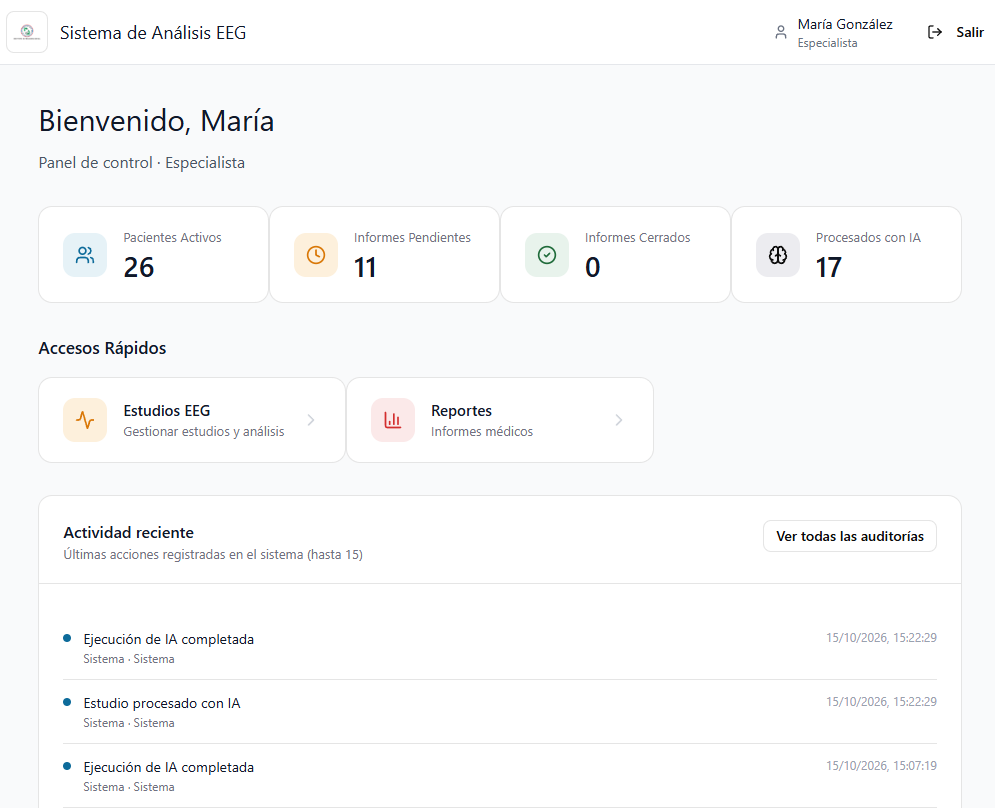
\includegraphics[width=\textwidth]{ThesisFigs/panel_principal_especialista.png}
    \caption{Organización del panel principal de EpilexIA
    correspondiente al perfil Especialista.}
    \label{fig:panel-principal-especialista}
\end{figure}


La navegación se estructura alrededor de las principales entidades y procesos administrados por EpilexIA. Las interfaces de estudios reúnen las operaciones relacionadas con su registro, seguimiento y acceso a los archivos asociados. Durante la creación de un estudio, el usuario puede seleccionar un paciente existente o registrar uno nuevo. Desde el entorno de un estudio, los usuarios autorizados pueden acceder a las funcionalidades de visualización de señales y revisión clínica.

La presentación de las acciones considera los
permisos del usuario autenticado. Por ejemplo,
las operaciones administrativas se orientan al
perfil Administrador, las actividades de registro
y preparación de estudios corresponden principalmente
al Técnico, y las herramientas de análisis e
informes clínicos se destinan al Especialista.
Esta diferenciación se refleja en los accesos,
controles y operaciones disponibles en cada pantalla.

Para mantener una experiencia de navegación
uniforme, la aplicación utiliza componentes
reutilizables en la presentación de información.
Entre ellos se encuentran tablas de registros,
formularios, controles de búsqueda, botones
de acción y elementos de navegación. La utilización
de estos componentes favorece la consistencia
visual y funcional entre las diferentes secciones
del sistema.

Las pantallas que presentan conjuntos de registros
incorporan mecanismos de búsqueda y organización
de resultados, según las características de cada
funcionalidad. Asimismo, los formularios permiten
introducir o actualizar información mediante
campos y controles específicos. Estas operaciones
se complementan con mecanismos de validación
y mensajes que comunican al usuario el estado
de las solicitudes realizadas.

La organización de la interfaz también considera
la adaptación a diferentes dimensiones de pantalla.
Para ello, la distribución de los elementos se
ajusta según el espacio disponible, procurando
conservar la accesibilidad de los controles y
la legibilidad de la información. No obstante,
las funcionalidades de análisis de señales EEG
requieren una superficie de visualización adecuada
debido a la cantidad de información gráfica
presentada simultáneamente.

En conjunto, esta organización proporciona
una estructura común para las distintas actividades
de EpilexIA y permite integrar la gestión
administrativa, el registro de estudios y la
revisión clínica dentro de una misma aplicación
web. Las características particulares de las
interfaces correspondientes a estos procesos
se desarrollan en los siguientes apartados.


\subsection{Interfaces de administración y gestión de estudios}

Las interfaces de administración y gestión de estudios de EpilexIA
permiten realizar las operaciones necesarias para organizar los
usuarios del sistema y administrar los estudios
electroencefalográficos. Estas pantallas utilizan formularios,
tablas de registros y controles de navegación que facilitan la
consulta y actualización de la información, de acuerdo con las
funcionalidades habilitadas para cada perfil.

En el ámbito administrativo, el sistema dispone de interfaces
orientadas a la gestión de usuarios y sus autorizaciones. Estas
permiten consultar la información de las cuentas, realizar
operaciones de administración y gestionar los roles y permisos
disponibles. La presentación de estas funcionalidades se organiza
mediante controles que facilitan la identificación de los registros
y la ejecución de las acciones correspondientes.

La administración de usuarios se encuentra diferenciada de las
actividades relacionadas con los estudios EEG. Mientras que el
perfil Administrador dispone de las funcionalidades de gestión de
cuentas y autorizaciones, los perfiles Técnico y Especialista
acceden principalmente a las operaciones de registro, consulta
y revisión de estudios, conforme a los permisos que tengan
asignados.

La gestión de estudios electroencefalográficos constituye una de
las funcionalidades centrales de la aplicación. La interfaz
correspondiente permite consultar los estudios registrados,
aplicar criterios de búsqueda y acceder a las operaciones
disponibles sobre cada uno de ellos. Los registros se presentan
mediante una tabla que incluye información del paciente, fechas
de creación y actualización, especialista responsable, estado
del estudio y procesamiento mediante inteligencia artificial.

La interfaz incorpora filtros que permiten localizar estudios
según diferentes criterios, entre ellos el nombre del paciente,
las fechas, el especialista responsable y el estado del estudio y del procesamiento mediante inteligencia artificial. Estos controles facilitan la identificación de
los registros y el seguimiento de las actividades relacionadas
con los estudios EEG.


La Figura~\ref{fig:gestion-estudios-eeg} presenta la interfaz
de gestión de estudios electroencefalográficos de EpilexIA,
en la que se observan los controles de búsqueda, los campos
de información y la opción de creación de nuevos estudios.


\begin{figure}[H]
    \centering
    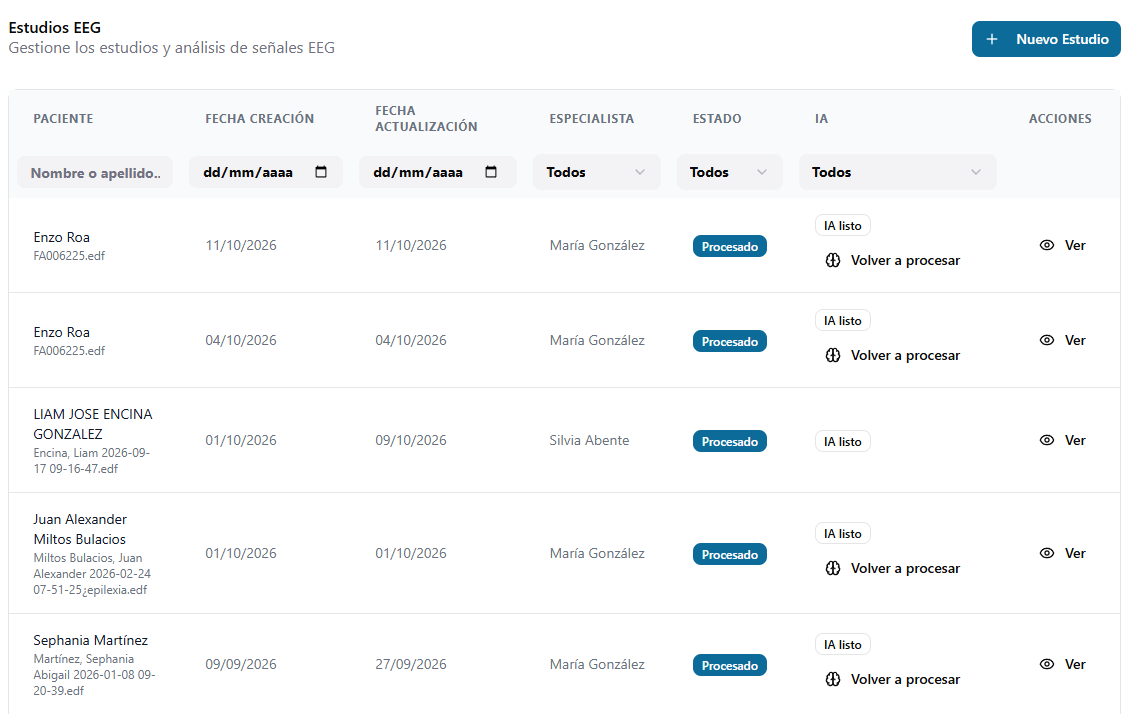
\includegraphics[width=\textwidth]{ThesisFigs/gestion_estudios_eeg.png}
    \caption{Interfaz de gestión de estudios EEG de EpilexIA.}
    \label{fig:gestion-estudios-eeg}
\end{figure}


El registro de un nuevo estudio se realiza mediante un formulario que permite seleccionar al paciente asociado e incorporar el archivo de señales EEG en formato EDF. La interfaz presenta diferencias según el perfil del usuario: en el caso del Técnico, se requiere seleccionar al especialista responsable del estudio, mientras que para el perfil Especialista dicho campo no se muestra. Asimismo, el formulario ofrece la posibilidad de adjuntar un video de monitoreo en formato MP4 o mediante archivos correspondientes a una grabación EZVideo.

Cuando el paciente requerido no se encuentra disponible en
el selector, la aplicación permite registrar uno nuevo sin
abandonar el proceso de creación del estudio. Esta operación
se realiza mediante un formulario que contempla datos de
identificación, información personal y datos de contacto.
De esta manera, el registro de pacientes se integra como
una funcionalidad complementaria a la creación de estudios
EEG, sin constituir un módulo independiente de gestión
de pacientes.

La Figura~\ref{fig:nuevo-estudio-eeg} presenta el formulario de creación de estudios EEG correspondiente al perfil Especialista. En ella se observan el campo de selección del paciente, así como los controles para incorporar el archivo EEG y, opcionalmente, un video de monitoreo.

\begin{figure}[H]
    \centering
    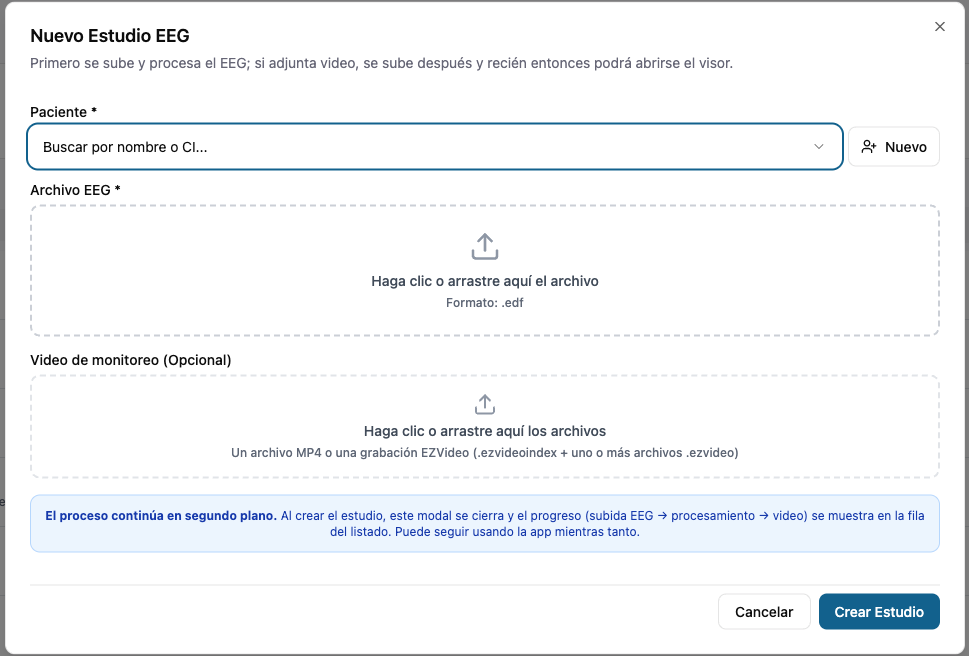
\includegraphics[width=\textwidth]{ThesisFigs/nuevo-estudio-eeg.png}
    \caption{Formulario de creación de estudios EEG correspondiente al perfil Especialista de EpilexIA.}
    \label{fig:nuevo-estudio-eeg}
\end{figure}

La creación del estudio contempla operaciones de carga y
procesamiento de archivos que continúan en segundo plano.
Una vez iniciado el procedimiento, el usuario puede seguir
utilizando la aplicación, mientras que el avance de las
operaciones se presenta en el listado de estudios. Este
mecanismo permite integrar la incorporación de archivos
y su preparación para la visualización posterior.

La organización de las pantallas de estudios también facilita
el acceso a las funcionalidades posteriores del proceso.
Desde un estudio registrado, los usuarios habilitados pueden
acceder a la visualización de señales electroencefalográficas
y a las herramientas de revisión clínica. De esta manera,
el registro inicial de los estudios se integra con las
actividades de análisis y elaboración de informes.

Las operaciones de consulta y actualización se complementan
con controles de búsqueda, acciones contextuales y mensajes
de estado. Estos elementos permiten localizar información,
identificar las operaciones disponibles y conocer el resultado
de las solicitudes realizadas, manteniendo una organización
consistente entre las distintas interfaces de gestión.

En conjunto, las interfaces de administración y gestión de
estudios proporcionan los medios necesarios para organizar
los usuarios del sistema, registrar estudios EEG e incorporar
los archivos utilizados durante la revisión clínica. Su
diseño establece una continuidad entre la administración
de cuentas, la preparación de estudios y el acceso a las
herramientas especializadas de análisis electroencefalográfico.


\subsection{Interfaz de visualización y análisis de señales EEG}

La interfaz de visualización y análisis de señales electroencefalográficas constituye uno de los componentes centrales de EpilexIA. Su diseño está orientado a facilitar la exploración de los registros EEG y proporcionar al especialista herramientas para examinar la actividad eléctrica cerebral, identificar posibles alteraciones y relacionar los hallazgos con la información asociada al estudio.

El acceso al visualizador se realiza desde la interfaz de gestión de estudios, mediante las acciones disponibles para cada registro. Una vez seleccionado un estudio, el sistema presenta las señales electroencefalográficas correspondientes, organizadas por canales y representadas gráficamente en función del tiempo. Esta disposición permite observar simultáneamente diferentes derivaciones y analizar su comportamiento durante el intervalo seleccionado.

La organización del visualizador contempla un área principal destinada a la representación de las señales EEG y un conjunto de controles que permiten modificar las condiciones de visualización. Estos elementos se distribuyen de manera que el usuario pueda realizar ajustes durante la exploración del registro sin abandonar el entorno de análisis.

La Figura~\ref{fig:interfaz-general-eeg} presenta la interfaz general de visualización y análisis de señales EEG de EpilexIA. En ella se observa la distribución del área de representación de las señales, los controles de configuración y navegación temporal, el panel de anomalías y el espacio destinado a la elaboración del informe médico.

\begin{figure}[H]
    \centering
    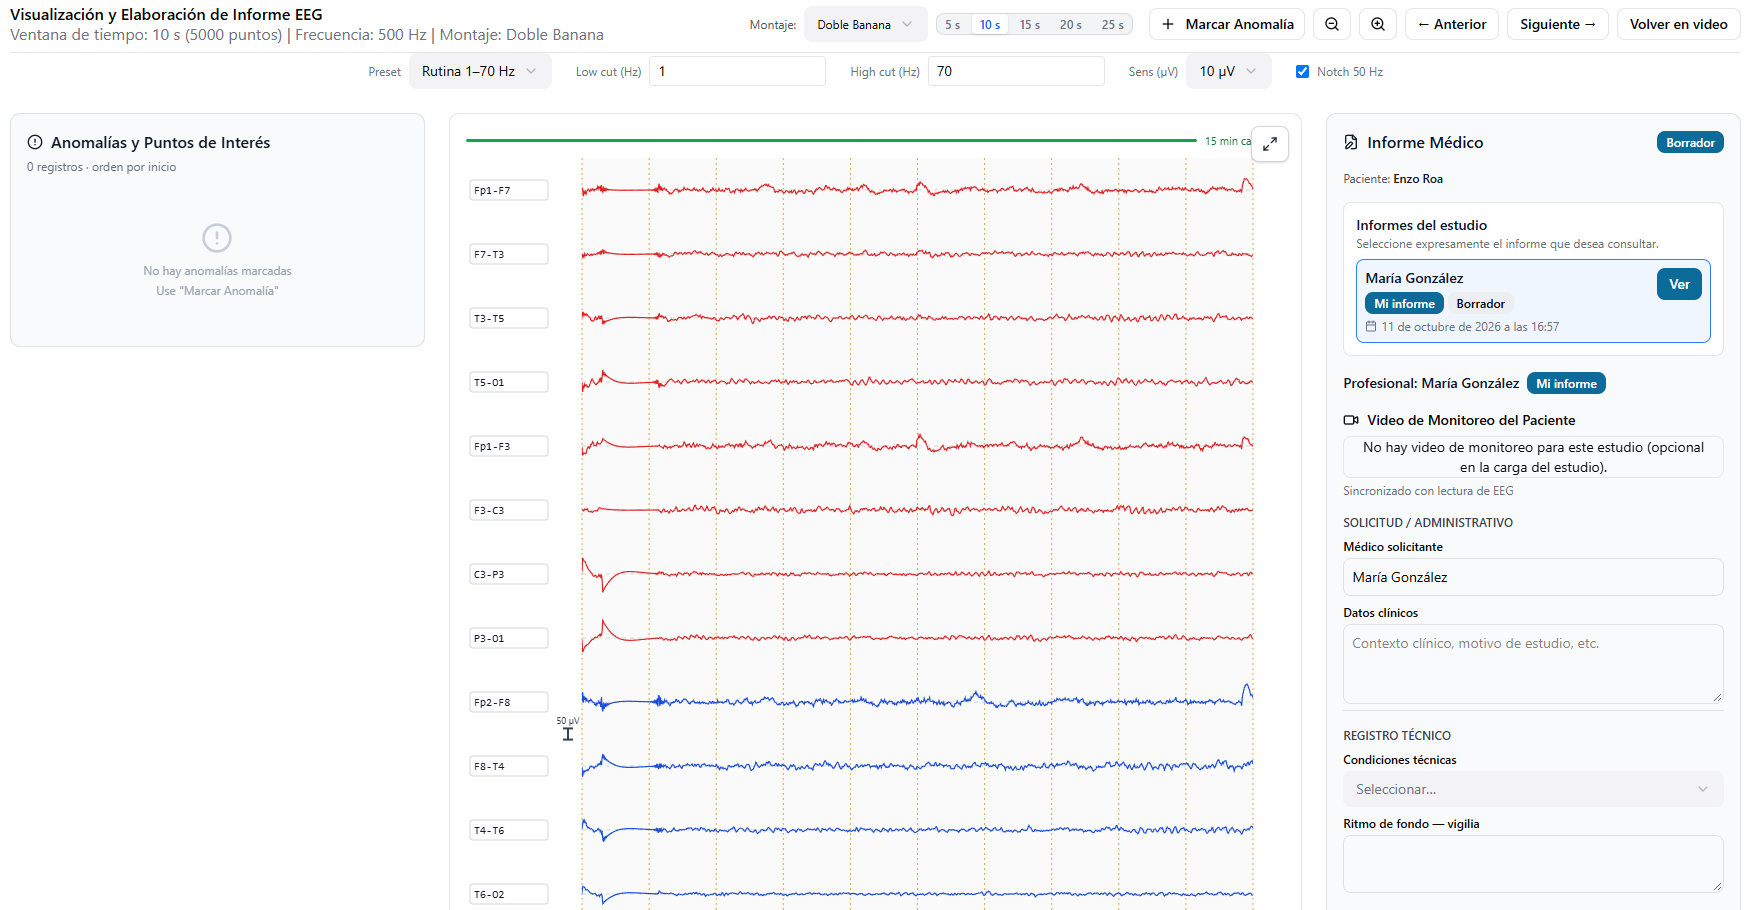
\includegraphics[width=\textwidth]{ThesisFigs/interfaz-general-eeg.png}
    \caption{Interfaz general de visualización y análisis de señales EEG de EpilexIA.}
    \label{fig:interfaz-general-eeg}
\end{figure}

Entre las funcionalidades disponibles se encuentra la navegación temporal, que permite desplazarse a lo largo del registro electroencefalográfico y examinar diferentes intervalos de tiempo. La interfaz incorpora controles para avanzar y retroceder por la señal, así como opciones para ajustar la ventana temporal representada. De esta manera, el especialista puede explorar tanto segmentos específicos como diferentes partes del estudio.

El visualizador también permite seleccionar montajes electroencefalográficos, mediante los cuales se determina la organización de las derivaciones presentadas. Esta funcionalidad facilita la revisión de las señales desde distintas configuraciones de canales, de acuerdo con las necesidades del análisis. Entre las configuraciones contempladas se encuentran los montajes bipolares y referenciales utilizados en la interpretación de registros EEG.

Otro elemento importante corresponde a los controles de filtrado y sensibilidad. Los filtros permiten ajustar la representación de las señales según los parámetros disponibles en la interfaz, mientras que el control de sensibilidad, expresado en microvoltios ($\mu$V), permite modificar la escala vertical de las ondas. Estos ajustes contribuyen a mejorar la observación de determinadas características de la actividad electroencefalográfica, sin modificar el archivo original del estudio.

Como herramienta complementaria, el visualizador incorpora un espectrograma que permite representar la distribución de la actividad de las señales EEG en función del tiempo y la frecuencia. Esta representación proporciona una perspectiva adicional para la exploración del registro electroencefalográfico.

Para ampliar el espacio destinado al análisis, EpilexIA incorpora un modo de pantalla completa. Esta funcionalidad permite visualizar las señales EEG en un área de mayor tamaño, reduciendo la presencia de otros elementos de la interfaz. El usuario puede continuar utilizando los controles de análisis disponibles y regresar posteriormente a la vista habitual.

La Figura~\ref{fig:visualizador-eeg-pantalla-completa} presenta el visualizador EEG en modo de pantalla completa, donde se observan simultáneamente múltiples canales electroencefalográficos, los controles laterales de navegación y el espectrograma ubicado en la parte inferior de la interfaz.

\begin{figure}[H]
    \centering
    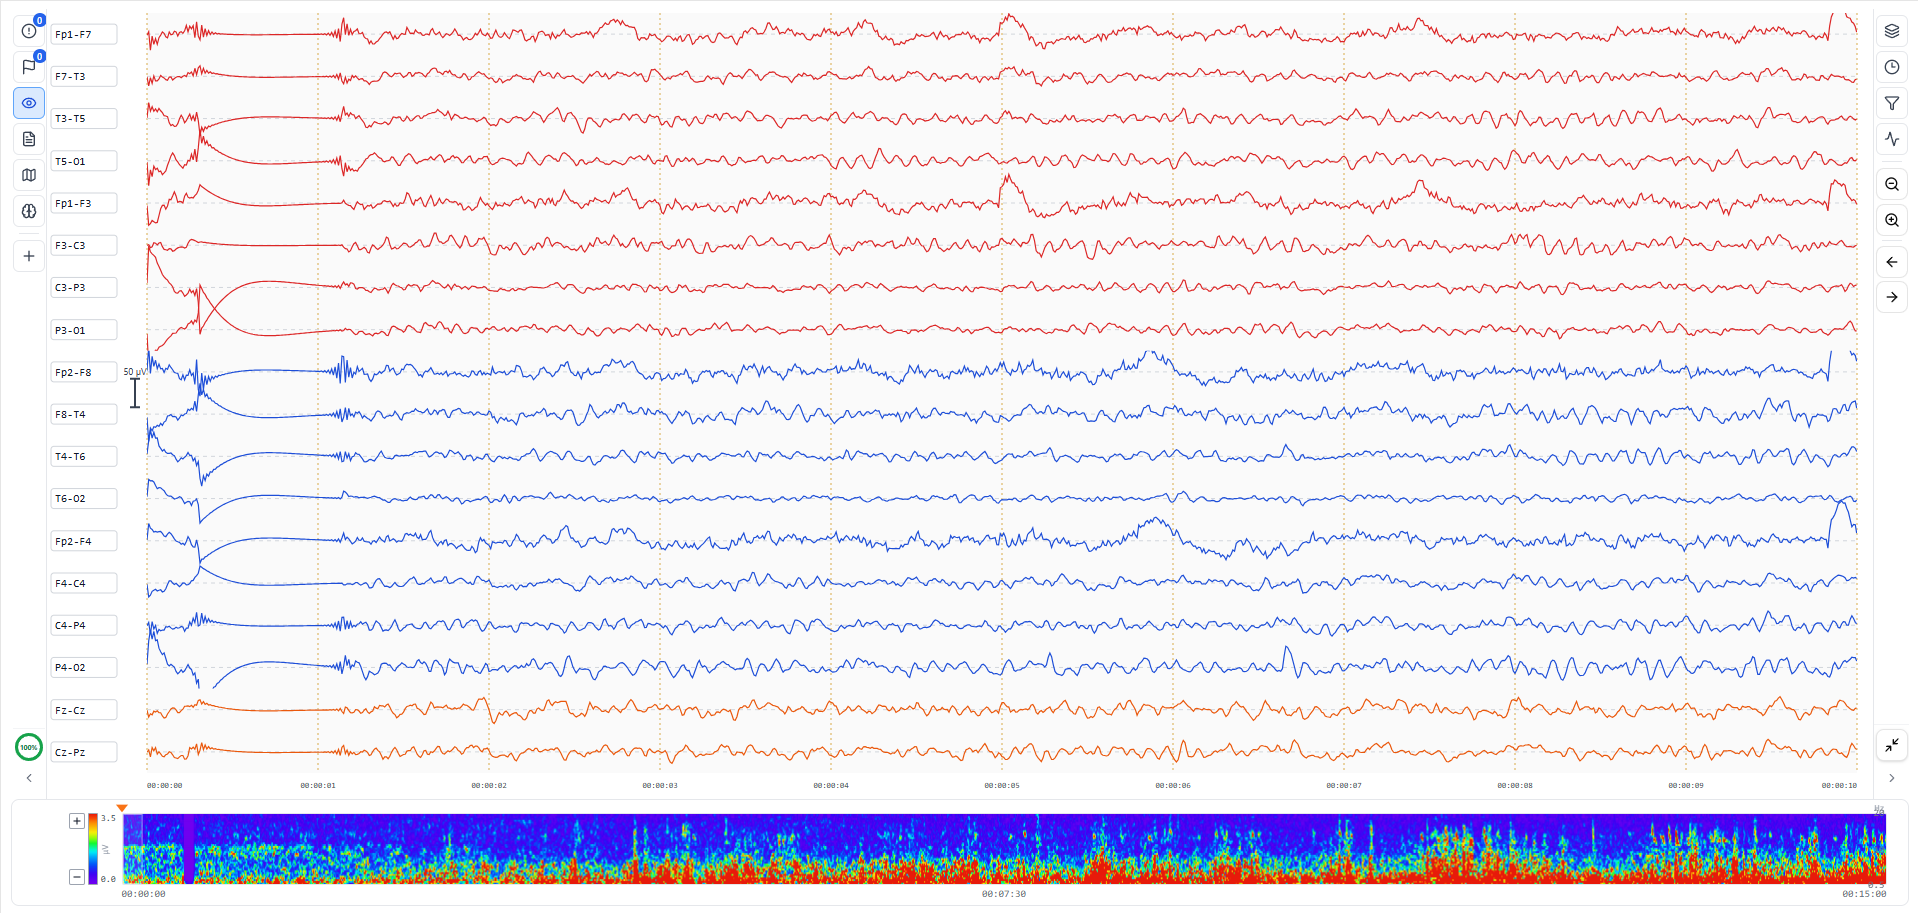
\includegraphics[width=\textwidth]{ThesisFigs/visualizador-eeg-pantalla-completa.png}
    \caption{Visualizador de señales EEG en modo de pantalla completa de EpilexIA.}
    \label{fig:visualizador-eeg-pantalla-completa}
\end{figure}

La interfaz también contempla la presentación de información relacionada con anomalías y eventos asociados al estudio. Estos elementos permiten vincular determinados intervalos del registro con observaciones realizadas durante su revisión. Asimismo, cuando existen resultados de procesamiento mediante inteligencia artificial, el especialista puede utilizarlos como información complementaria para orientar la exploración de segmentos de interés.

La visualización de las señales se integra con las demás funcionalidades de revisión clínica de EpilexIA. De esta manera, el especialista puede examinar los registros electroencefalográficos y relacionar los hallazgos observados con las actividades de documentación y elaboración de informes médicos correspondientes al estudio.

En conjunto, el diseño del visualizador EEG reúne herramientas de navegación, configuración y exploración de señales dentro de una misma interfaz. Su organización busca facilitar el análisis de registros electroencefalográficos y proporcionar un entorno de trabajo que apoye la revisión clínica realizada por el especialista.

\subsection[Interfaces de revisión clínica y elaboración de informes médicos]
{Interfaces de revisión clínica y elaboración de\\informes médicos}

Las interfaces de revisión clínica y elaboración de informes médicos de EpilexIA están orientadas a facilitar la documentación de los hallazgos identificados durante el análisis de los estudios electroencefalográficos. Estas funcionalidades permiten al especialista relacionar las observaciones realizadas sobre las señales EEG con la información clínica correspondiente y organizar los resultados de su evaluación dentro de un mismo entorno de trabajo.

La revisión clínica se desarrolla a partir de los estudios registrados en el sistema. Una vez que el especialista accede a un estudio, dispone de herramientas para examinar las señales electroencefalográficas, identificar segmentos de interés y registrar observaciones relacionadas con posibles alteraciones. Estas operaciones se integran con el visualizador EEG, permitiendo mantener una relación entre los hallazgos documentados y los intervalos temporales del registro.

Entre las funcionalidades disponibles se encuentra el registro de anomalías y eventos asociados al estudio. Estas herramientas permiten documentar situaciones identificadas durante la exploración de las señales y vincularlas con determinados segmentos del registro electroencefalográfico. La información registrada constituye un recurso de apoyo para la revisión posterior y la elaboración del informe médico.


Cuando un estudio dispone de resultados de inteligencia artificial previamente almacenados, la interfaz permite consultar los intervalos señalados en dichos registros. Estos resultados se presentan como información complementaria para orientar la revisión del especialista, quien conserva la responsabilidad de examinar las señales y determinar la relevancia clínica de los hallazgos. De esta manera, el sistema integra el apoyo automatizado sin sustituir la interpretación realizada por el profesional.


La Figura~\ref{fig:panel-anomalias-ia} presenta el panel de anomalías y puntos de interés de EpilexIA, en el que se observan los intervalos identificados mediante inteligencia artificial, sus respectivas referencias temporales y los controles disponibles para su consulta. Asimismo, la interfaz incorpora filtros que permiten distinguir entre los registros generados automáticamente y aquellos incorporados de forma manual.

\begin{figure}[H]
    \centering
    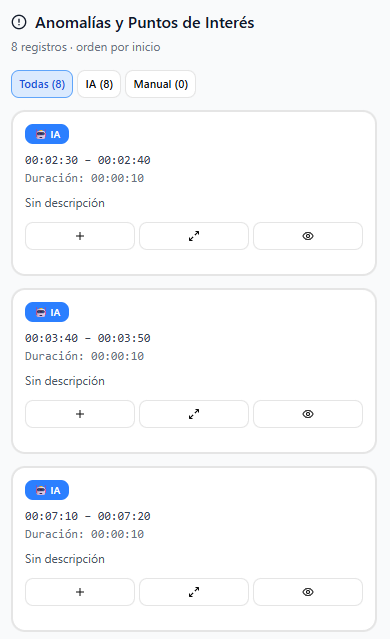
\includegraphics[width=0.55\textwidth]{ThesisFigs/panel_anomalias_ia.png}
    \caption{Panel de anomalías y puntos de interés de EpilexIA con resultados de inteligencia artificial.}
    \label{fig:panel-anomalias-ia}
\end{figure}

La elaboración de informes médicos constituye otra funcionalidad central de este entorno. EpilexIA incorpora una interfaz que permite registrar y actualizar la información correspondiente a la evaluación clínica del estudio. Los formularios se organizan mediante secciones destinadas a documentar los antecedentes y datos clínicos pertinentes, las observaciones sobre el registro electroencefalográfico y las conclusiones del especialista.

La interfaz de informes se encuentra vinculada al estudio EEG correspondiente, lo que facilita la consulta de las señales durante la elaboración del documento. Esta integración permite que el especialista mantenga disponibles los elementos necesarios para relacionar las observaciones realizadas con la información incorporada al informe médico.


El sistema contempla la participación de diferentes Especialistas autorizados en la revisión de un mismo estudio. Cada Especialista puede elaborar un único informe médico propio por estudio, manteniendo diferenciados los registros correspondientes a cada autor. Esta organización permite conservar la individualidad de las evaluaciones y garantiza que ningún Especialista pueda modificar el contenido de un informe perteneciente a otro profesional.


Los informes médicos disponen de estados que permiten distinguir aquellos que se encuentran en Borrador de los que han sido Cerrados. Durante la etapa de borrador, el especialista puede continuar registrando y actualizando la información correspondiente. Una vez cerrado el informe, se aplican las restricciones establecidas por el sistema para impedir modificaciones posteriores.

La presentación de los informes incorpora controles para seleccionar los documentos asociados al estudio y consultar su contenido, de acuerdo con los permisos del usuario. Asimismo, las acciones de creación, edición y cierre se encuentran diferenciadas según el estado del informe y las autorizaciones correspondientes al especialista.

La Figura~\ref{fig:interfaz-informe-medico} presenta la interfaz de elaboración de informes médicos de EpilexIA. En ella se observan las secciones destinadas al registro de información administrativa, datos clínicos, condiciones técnicas, hallazgos ictales e interictales, conclusiones y observaciones. Asimismo, se muestran los controles disponibles para guardar el informe, consultar su vista previa y proceder a su cierre.


\begin{figure}[H]
    \centering

    \begin{minipage}[t]{0.46\textwidth}
        \vspace{0pt}
        \centering
        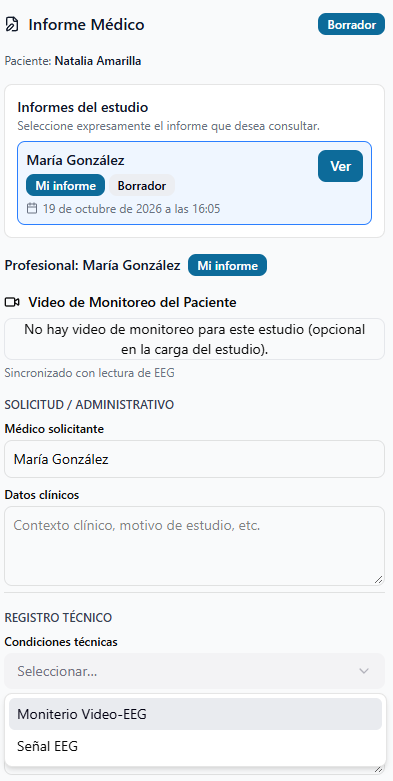
\includegraphics[width=\linewidth]{ThesisFigs/informe_medico_superior.png}
    \end{minipage}
    \hfill
    \begin{minipage}[t]{0.46\textwidth}
        \vspace{0pt}
        \centering
        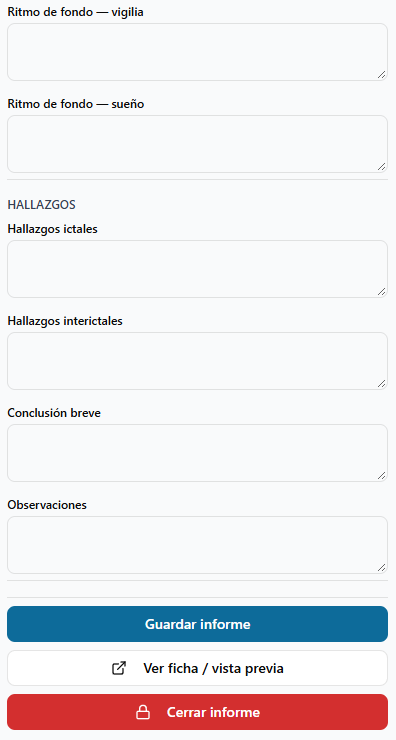
\includegraphics[width=\linewidth]{ThesisFigs/informe_medico_inferior.png}
    \end{minipage}

    \caption{Interfaz de elaboración de informes médicos de EpilexIA.}
    \label{fig:interfaz-informe-medico}
\end{figure}

En conjunto, las interfaces de revisión clínica y elaboración de informes médicos permiten integrar la identificación de hallazgos, el registro de anomalías y eventos, la consulta de resultados de inteligencia artificial y la documentación de las evaluaciones profesionales. Su diseño busca proporcionar un entorno de trabajo organizado que facilite la continuidad entre el análisis de las señales EEG y la elaboración de los informes médicos asociados a cada estudio.